% Created by tikzDevice version 0.12.4 on 2023-07-16 12:55:38
% !TEX encoding = UTF-8 Unicode
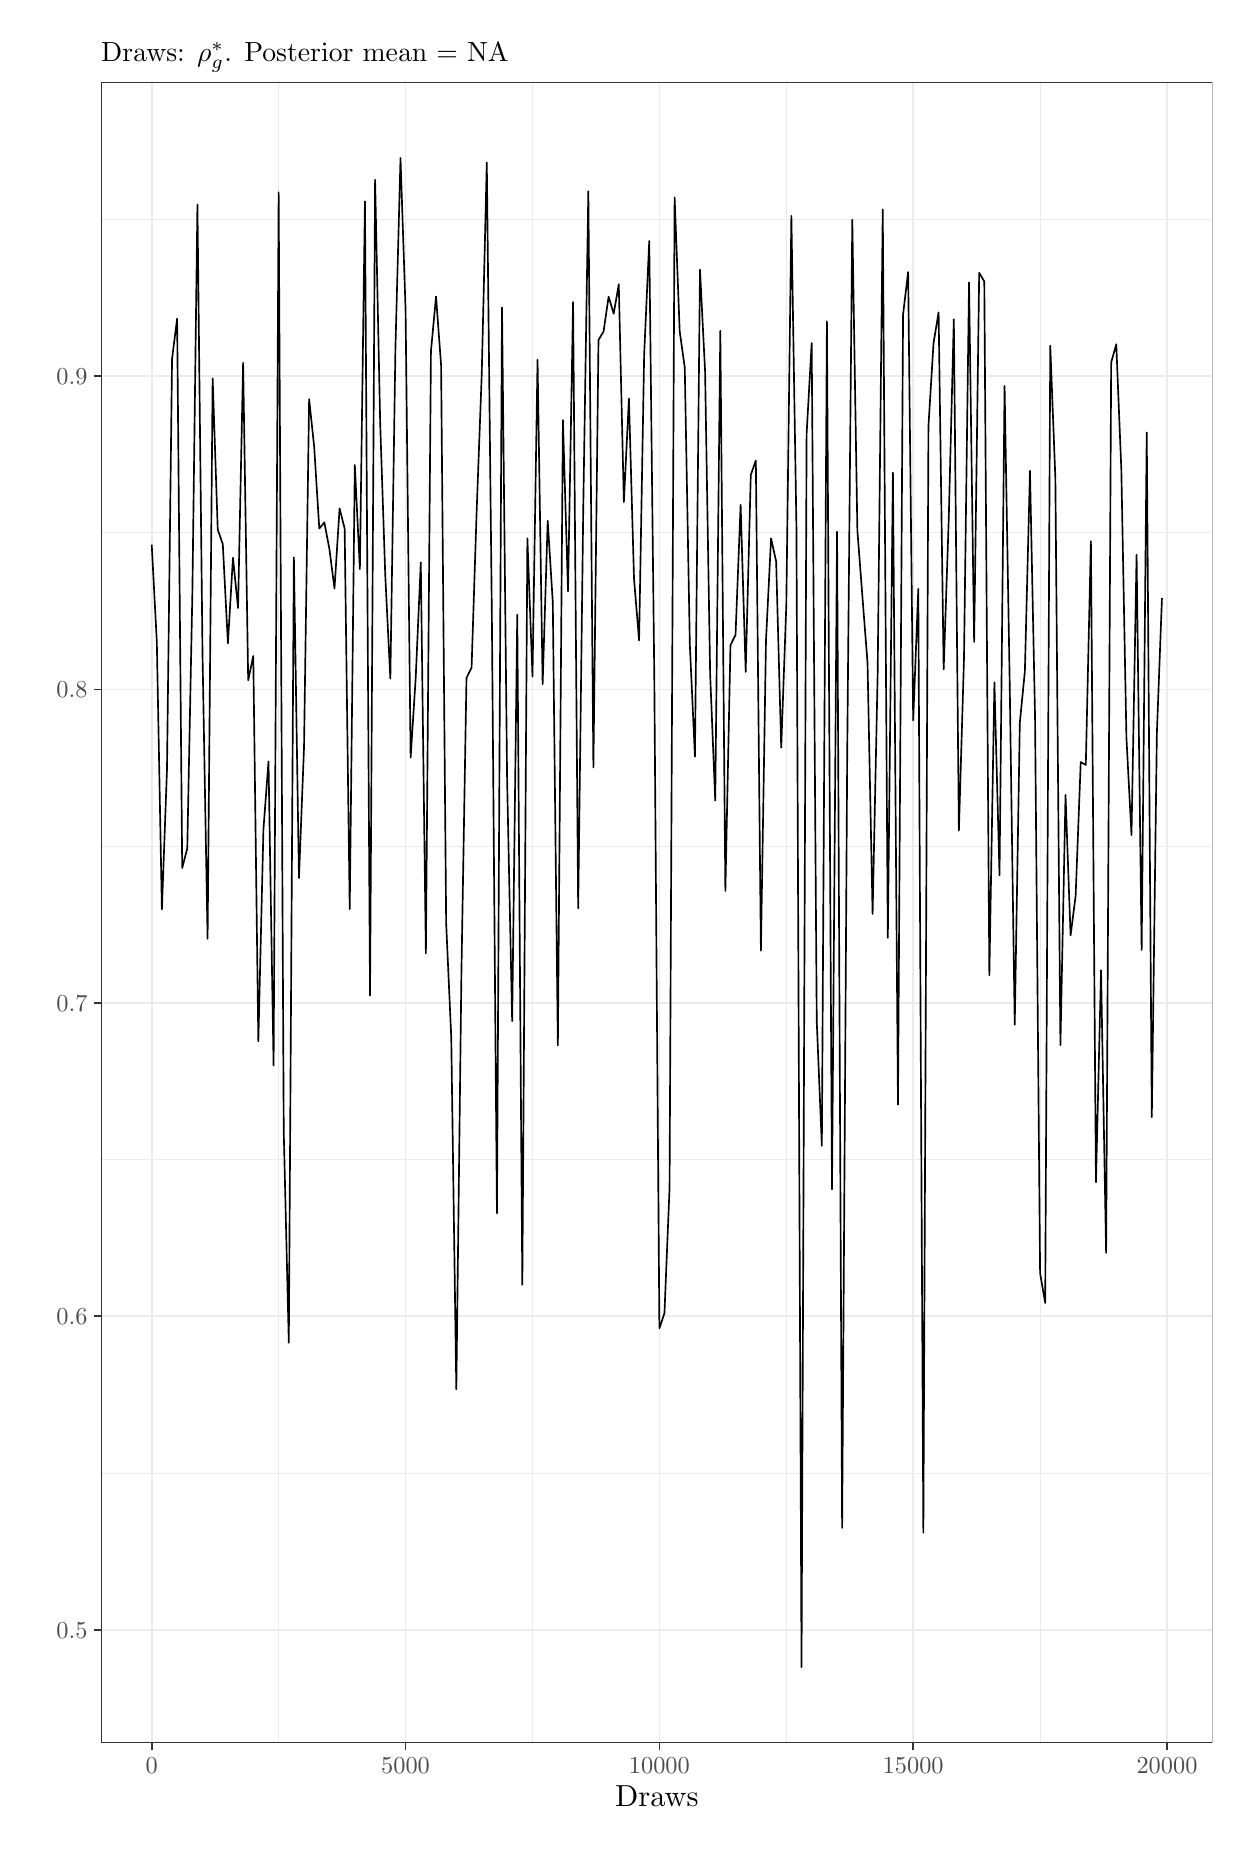
\begin{tikzpicture}[x=1pt,y=1pt]
\definecolor{fillColor}{RGB}{255,255,255}
\path[use as bounding box,fill=fillColor,fill opacity=0.00] (0,0) rectangle (433.62,650.43);
\begin{scope}
\path[clip] (  0.00,  0.00) rectangle (433.62,650.43);
\definecolor{drawColor}{RGB}{255,255,255}
\definecolor{fillColor}{RGB}{255,255,255}

\path[draw=drawColor,line width= 0.6pt,line join=round,line cap=round,fill=fillColor] (  0.00,  0.00) rectangle (433.62,650.43);
\end{scope}
\begin{scope}
\path[clip] ( 26.58, 30.69) rectangle (428.12,630.60);
\definecolor{fillColor}{RGB}{255,255,255}

\path[fill=fillColor] ( 26.58, 30.69) rectangle (428.12,630.60);
\definecolor{drawColor}{gray}{0.92}

\path[draw=drawColor,line width= 0.3pt,line join=round] ( 26.58,128.16) --
	(428.12,128.16);

\path[draw=drawColor,line width= 0.3pt,line join=round] ( 26.58,241.41) --
	(428.12,241.41);

\path[draw=drawColor,line width= 0.3pt,line join=round] ( 26.58,354.65) --
	(428.12,354.65);

\path[draw=drawColor,line width= 0.3pt,line join=round] ( 26.58,467.90) --
	(428.12,467.90);

\path[draw=drawColor,line width= 0.3pt,line join=round] ( 26.58,581.15) --
	(428.12,581.15);

\path[draw=drawColor,line width= 0.3pt,line join=round] ( 90.69, 30.69) --
	( 90.69,630.60);

\path[draw=drawColor,line width= 0.3pt,line join=round] (182.41, 30.69) --
	(182.41,630.60);

\path[draw=drawColor,line width= 0.3pt,line join=round] (274.13, 30.69) --
	(274.13,630.60);

\path[draw=drawColor,line width= 0.3pt,line join=round] (365.84, 30.69) --
	(365.84,630.60);

\path[draw=drawColor,line width= 0.6pt,line join=round] ( 26.58, 71.54) --
	(428.12, 71.54);

\path[draw=drawColor,line width= 0.6pt,line join=round] ( 26.58,184.79) --
	(428.12,184.79);

\path[draw=drawColor,line width= 0.6pt,line join=round] ( 26.58,298.03) --
	(428.12,298.03);

\path[draw=drawColor,line width= 0.6pt,line join=round] ( 26.58,411.28) --
	(428.12,411.28);

\path[draw=drawColor,line width= 0.6pt,line join=round] ( 26.58,524.52) --
	(428.12,524.52);

\path[draw=drawColor,line width= 0.6pt,line join=round] ( 44.83, 30.69) --
	( 44.83,630.60);

\path[draw=drawColor,line width= 0.6pt,line join=round] (136.55, 30.69) --
	(136.55,630.60);

\path[draw=drawColor,line width= 0.6pt,line join=round] (228.27, 30.69) --
	(228.27,630.60);

\path[draw=drawColor,line width= 0.6pt,line join=round] (319.98, 30.69) --
	(319.98,630.60);

\path[draw=drawColor,line width= 0.6pt,line join=round] (411.70, 30.69) --
	(411.70,630.60);
\definecolor{drawColor}{RGB}{0,0,0}

\path[draw=drawColor,line width= 0.6pt,line join=round] ( 44.83,463.59) --
	( 46.67,428.37) --
	( 48.50,331.84) --
	( 50.34,382.39) --
	( 52.17,530.69) --
	( 54.00,545.31) --
	( 55.84,346.78) --
	( 57.67,353.85) --
	( 59.51,446.02) --
	( 61.34,586.54) --
	( 63.18,423.93) --
	( 65.01,321.20) --
	( 66.84,523.73) --
	( 68.68,469.08) --
	( 70.51,463.77) --
	( 72.35,427.96) --
	( 74.18,458.88) --
	( 76.02,440.71) --
	( 77.85,529.30) --
	( 79.68,414.62) --
	( 81.52,423.39) --
	( 83.35,284.11) --
	( 85.19,360.72) --
	( 87.02,385.30) --
	( 88.86,275.40) --
	( 90.69,590.93) --
	( 92.53,251.55) --
	( 94.36,175.19) --
	( 96.19,459.07) --
	( 98.03,343.15) --
	( 99.86,390.52) --
	(101.70,516.22) --
	(103.53,498.94) --
	(105.37,469.45) --
	(107.20,471.65) --
	(109.03,462.04) --
	(110.87,447.74) --
	(112.70,476.73) --
	(114.54,469.39) --
	(116.37,331.90) --
	(118.21,492.39) --
	(120.04,454.76) --
	(121.87,587.66) --
	(123.71,300.66) --
	(125.54,595.48) --
	(127.38,507.41) --
	(129.21,452.62) --
	(131.05,415.22) --
	(132.88,534.30) --
	(134.72,603.33) --
	(136.55,548.60) --
	(138.38,386.65) --
	(140.22,415.59) --
	(142.05,457.21) --
	(143.89,315.90) --
	(145.72,533.48) --
	(147.56,553.26) --
	(149.39,528.40) --
	(151.22,326.80) --
	(153.06,285.59) --
	(154.89,158.39) --
	(156.73,308.89) --
	(158.56,415.45) --
	(160.40,419.20) --
	(162.23,475.51) --
	(164.06,524.78) --
	(165.90,601.71) --
	(167.73,438.20) --
	(169.57,221.98) --
	(171.40,549.29) --
	(173.24,378.87) --
	(175.07,291.44) --
	(176.91,438.26) --
	(178.74,196.17) --
	(180.57,465.86) --
	(182.41,415.97) --
	(184.24,530.46) --
	(186.08,413.22) --
	(187.91,472.20) --
	(189.75,442.79) --
	(191.58,282.66) --
	(193.41,508.63) --
	(195.25,446.73) --
	(197.08,551.25) --
	(198.92,332.21) --
	(200.75,476.23) --
	(202.59,591.31) --
	(204.42,383.08) --
	(206.26,537.58) --
	(208.09,540.62) --
	(209.92,553.20) --
	(211.76,547.06) --
	(213.59,557.70) --
	(215.43,479.00) --
	(217.26,516.41) --
	(219.10,451.31) --
	(220.93,429.01) --
	(222.76,532.12) --
	(224.60,573.35) --
	(226.43,415.71) --
	(228.27,180.46) --
	(230.10,185.93) --
	(231.94,231.14) --
	(233.77,589.09) --
	(235.60,540.78) --
	(237.44,527.55) --
	(239.27,427.52) --
	(241.11,387.02) --
	(242.94,562.96) --
	(244.78,526.23) --
	(246.61,416.77) --
	(248.45,371.11) --
	(250.28,540.87) --
	(252.11,338.45) --
	(253.95,427.28) --
	(255.78,430.97) --
	(257.62,477.97) --
	(259.45,417.62) --
	(261.29,488.78) --
	(263.12,494.01) --
	(264.95,316.90) --
	(266.79,429.06) --
	(268.62,465.86) --
	(270.46,457.55) --
	(272.29,390.25) --
	(274.13,441.83) --
	(275.96,582.42) --
	(277.79,469.68) --
	(279.63, 57.95) --
	(281.46,503.56) --
	(283.30,536.46) --
	(285.13,291.41) --
	(286.97,246.39) --
	(288.80,544.33) --
	(290.64,230.64) --
	(292.47,468.28) --
	(294.30,108.31) --
	(296.14,388.24) --
	(297.97,581.03) --
	(299.81,468.69) --
	(301.64,444.72) --
	(303.48,420.86) --
	(305.31,330.17) --
	(307.14,416.96) --
	(308.98,584.76) --
	(310.81,321.51) --
	(312.65,489.66) --
	(314.48,261.26) --
	(316.32,546.81) --
	(318.15,562.12) --
	(319.98,400.11) --
	(321.82,447.65) --
	(323.65,106.63) --
	(325.49,506.45) --
	(327.32,536.38) --
	(329.16,547.56) --
	(330.99,418.51) --
	(332.83,472.99) --
	(334.66,545.06) --
	(336.49,360.28) --
	(338.33,422.33) --
	(340.16,558.34) --
	(342.00,428.50) --
	(343.83,561.86) --
	(345.67,558.72) --
	(347.50,308.01) --
	(349.33,413.84) --
	(351.17,344.16) --
	(353.00,520.96) --
	(354.84,414.36) --
	(356.67,290.09) --
	(358.51,399.24) --
	(360.34,417.94) --
	(362.18,490.29) --
	(364.01,401.49) --
	(365.84,200.30) --
	(367.68,189.61) --
	(369.51,535.50) --
	(371.35,487.65) --
	(373.18,282.78) --
	(375.02,373.15) --
	(376.85,322.42) --
	(378.68,336.74) --
	(380.52,385.08) --
	(382.35,383.99) --
	(384.19,464.86) --
	(386.02,233.18) --
	(387.86,309.83) --
	(389.69,207.67) --
	(391.52,529.45) --
	(393.36,536.03) --
	(395.19,490.71) --
	(397.03,393.89) --
	(398.86,358.64) --
	(400.70,459.94) --
	(402.53,317.13) --
	(404.37,504.19) --
	(406.20,256.73) --
	(408.03,395.41) --
	(409.87,444.33);
\definecolor{drawColor}{gray}{0.20}

\path[draw=drawColor,line width= 0.6pt,line join=round,line cap=round] ( 26.58, 30.69) rectangle (428.12,630.60);
\end{scope}
\begin{scope}
\path[clip] (  0.00,  0.00) rectangle (433.62,650.43);
\definecolor{drawColor}{gray}{0.30}

\node[text=drawColor,anchor=base east,inner sep=0pt, outer sep=0pt, scale=  0.88] at ( 21.63, 68.51) {0.5};

\node[text=drawColor,anchor=base east,inner sep=0pt, outer sep=0pt, scale=  0.88] at ( 21.63,181.76) {0.6};

\node[text=drawColor,anchor=base east,inner sep=0pt, outer sep=0pt, scale=  0.88] at ( 21.63,295.00) {0.7};

\node[text=drawColor,anchor=base east,inner sep=0pt, outer sep=0pt, scale=  0.88] at ( 21.63,408.25) {0.8};

\node[text=drawColor,anchor=base east,inner sep=0pt, outer sep=0pt, scale=  0.88] at ( 21.63,521.49) {0.9};
\end{scope}
\begin{scope}
\path[clip] (  0.00,  0.00) rectangle (433.62,650.43);
\definecolor{drawColor}{gray}{0.20}

\path[draw=drawColor,line width= 0.6pt,line join=round] ( 23.83, 71.54) --
	( 26.58, 71.54);

\path[draw=drawColor,line width= 0.6pt,line join=round] ( 23.83,184.79) --
	( 26.58,184.79);

\path[draw=drawColor,line width= 0.6pt,line join=round] ( 23.83,298.03) --
	( 26.58,298.03);

\path[draw=drawColor,line width= 0.6pt,line join=round] ( 23.83,411.28) --
	( 26.58,411.28);

\path[draw=drawColor,line width= 0.6pt,line join=round] ( 23.83,524.52) --
	( 26.58,524.52);
\end{scope}
\begin{scope}
\path[clip] (  0.00,  0.00) rectangle (433.62,650.43);
\definecolor{drawColor}{gray}{0.20}

\path[draw=drawColor,line width= 0.6pt,line join=round] ( 44.83, 27.94) --
	( 44.83, 30.69);

\path[draw=drawColor,line width= 0.6pt,line join=round] (136.55, 27.94) --
	(136.55, 30.69);

\path[draw=drawColor,line width= 0.6pt,line join=round] (228.27, 27.94) --
	(228.27, 30.69);

\path[draw=drawColor,line width= 0.6pt,line join=round] (319.98, 27.94) --
	(319.98, 30.69);

\path[draw=drawColor,line width= 0.6pt,line join=round] (411.70, 27.94) --
	(411.70, 30.69);
\end{scope}
\begin{scope}
\path[clip] (  0.00,  0.00) rectangle (433.62,650.43);
\definecolor{drawColor}{gray}{0.30}

\node[text=drawColor,anchor=base,inner sep=0pt, outer sep=0pt, scale=  0.88] at ( 44.83, 19.68) {0};

\node[text=drawColor,anchor=base,inner sep=0pt, outer sep=0pt, scale=  0.88] at (136.55, 19.68) {5000};

\node[text=drawColor,anchor=base,inner sep=0pt, outer sep=0pt, scale=  0.88] at (228.27, 19.68) {10000};

\node[text=drawColor,anchor=base,inner sep=0pt, outer sep=0pt, scale=  0.88] at (319.98, 19.68) {15000};

\node[text=drawColor,anchor=base,inner sep=0pt, outer sep=0pt, scale=  0.88] at (411.70, 19.68) {20000};
\end{scope}
\begin{scope}
\path[clip] (  0.00,  0.00) rectangle (433.62,650.43);
\definecolor{drawColor}{RGB}{0,0,0}

\node[text=drawColor,anchor=base,inner sep=0pt, outer sep=0pt, scale=  1.10] at (227.35,  7.64) {Draws};
\end{scope}
\begin{scope}
\path[clip] (  0.00,  0.00) rectangle (433.62,650.43);
\definecolor{drawColor}{RGB}{0,0,0}

\node[text=drawColor,anchor=base west,inner sep=0pt, outer sep=0pt, scale=  1.00] at ( 26.58,638.04) {Draws: $\rho_g^*$. Posterior mean = NA};
\end{scope}
\end{tikzpicture}
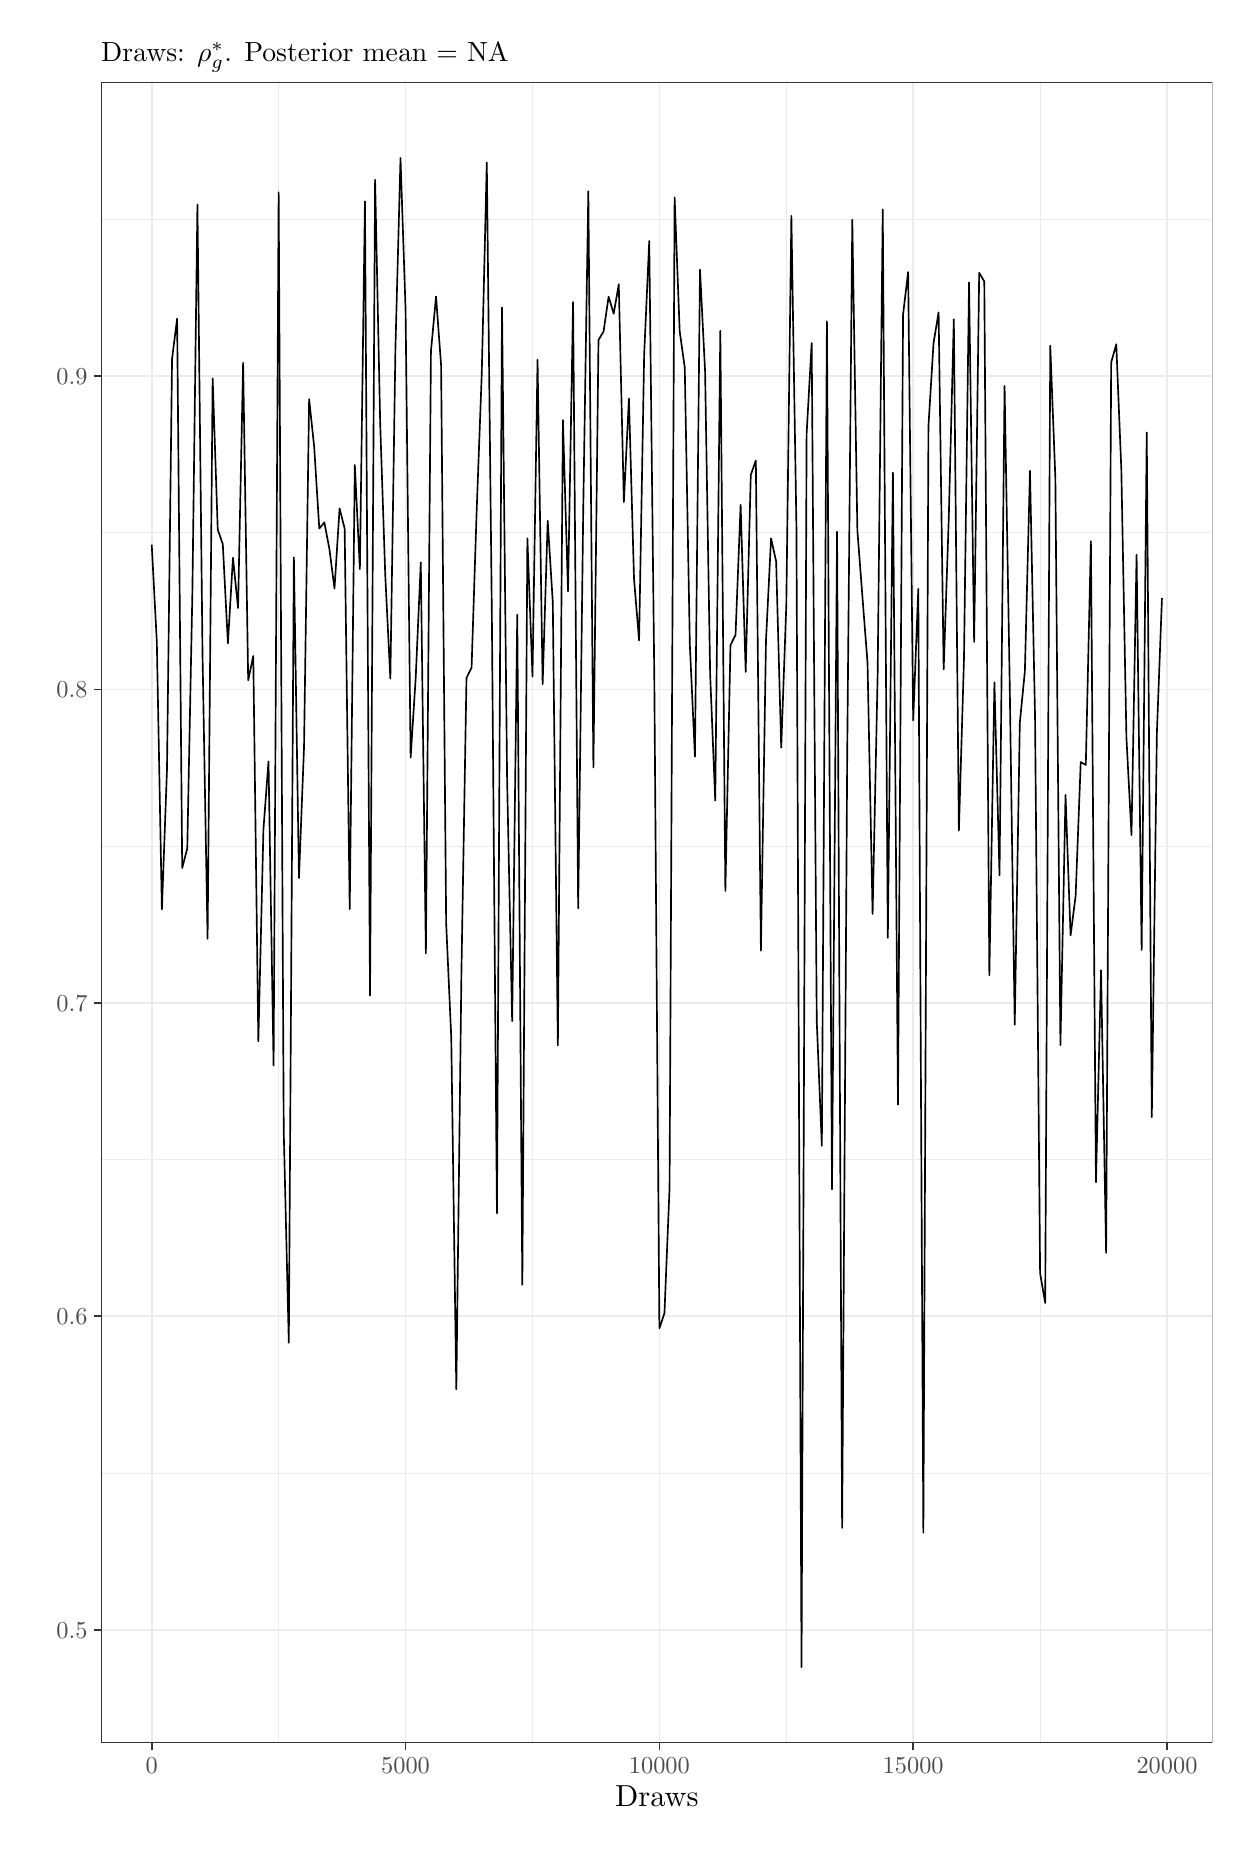
\begin{tikzpicture}[x=1pt,y=1pt]
\definecolor{fillColor}{RGB}{255,255,255}
\path[use as bounding box,fill=fillColor,fill opacity=0.00] (0,0) rectangle (433.62,650.43);
\begin{scope}
\path[clip] (  0.00,  0.00) rectangle (433.62,650.43);
\definecolor{drawColor}{RGB}{255,255,255}
\definecolor{fillColor}{RGB}{255,255,255}

\path[draw=drawColor,line width= 0.6pt,line join=round,line cap=round,fill=fillColor] (  0.00,  0.00) rectangle (433.62,650.43);
\end{scope}
\begin{scope}
\path[clip] ( 26.58, 30.69) rectangle (428.12,630.60);
\definecolor{fillColor}{RGB}{255,255,255}

\path[fill=fillColor] ( 26.58, 30.69) rectangle (428.12,630.60);
\definecolor{drawColor}{gray}{0.92}

\path[draw=drawColor,line width= 0.3pt,line join=round] ( 26.58,128.16) --
	(428.12,128.16);

\path[draw=drawColor,line width= 0.3pt,line join=round] ( 26.58,241.41) --
	(428.12,241.41);

\path[draw=drawColor,line width= 0.3pt,line join=round] ( 26.58,354.65) --
	(428.12,354.65);

\path[draw=drawColor,line width= 0.3pt,line join=round] ( 26.58,467.90) --
	(428.12,467.90);

\path[draw=drawColor,line width= 0.3pt,line join=round] ( 26.58,581.15) --
	(428.12,581.15);

\path[draw=drawColor,line width= 0.3pt,line join=round] ( 90.69, 30.69) --
	( 90.69,630.60);

\path[draw=drawColor,line width= 0.3pt,line join=round] (182.41, 30.69) --
	(182.41,630.60);

\path[draw=drawColor,line width= 0.3pt,line join=round] (274.13, 30.69) --
	(274.13,630.60);

\path[draw=drawColor,line width= 0.3pt,line join=round] (365.84, 30.69) --
	(365.84,630.60);

\path[draw=drawColor,line width= 0.6pt,line join=round] ( 26.58, 71.54) --
	(428.12, 71.54);

\path[draw=drawColor,line width= 0.6pt,line join=round] ( 26.58,184.79) --
	(428.12,184.79);

\path[draw=drawColor,line width= 0.6pt,line join=round] ( 26.58,298.03) --
	(428.12,298.03);

\path[draw=drawColor,line width= 0.6pt,line join=round] ( 26.58,411.28) --
	(428.12,411.28);

\path[draw=drawColor,line width= 0.6pt,line join=round] ( 26.58,524.52) --
	(428.12,524.52);

\path[draw=drawColor,line width= 0.6pt,line join=round] ( 44.83, 30.69) --
	( 44.83,630.60);

\path[draw=drawColor,line width= 0.6pt,line join=round] (136.55, 30.69) --
	(136.55,630.60);

\path[draw=drawColor,line width= 0.6pt,line join=round] (228.27, 30.69) --
	(228.27,630.60);

\path[draw=drawColor,line width= 0.6pt,line join=round] (319.98, 30.69) --
	(319.98,630.60);

\path[draw=drawColor,line width= 0.6pt,line join=round] (411.70, 30.69) --
	(411.70,630.60);
\definecolor{drawColor}{RGB}{0,0,0}

\path[draw=drawColor,line width= 0.6pt,line join=round] ( 44.83,463.59) --
	( 46.67,428.37) --
	( 48.50,331.84) --
	( 50.34,382.39) --
	( 52.17,530.69) --
	( 54.00,545.31) --
	( 55.84,346.78) --
	( 57.67,353.85) --
	( 59.51,446.02) --
	( 61.34,586.54) --
	( 63.18,423.93) --
	( 65.01,321.20) --
	( 66.84,523.73) --
	( 68.68,469.08) --
	( 70.51,463.77) --
	( 72.35,427.96) --
	( 74.18,458.88) --
	( 76.02,440.71) --
	( 77.85,529.30) --
	( 79.68,414.62) --
	( 81.52,423.39) --
	( 83.35,284.11) --
	( 85.19,360.72) --
	( 87.02,385.30) --
	( 88.86,275.40) --
	( 90.69,590.93) --
	( 92.53,251.55) --
	( 94.36,175.19) --
	( 96.19,459.07) --
	( 98.03,343.15) --
	( 99.86,390.52) --
	(101.70,516.22) --
	(103.53,498.94) --
	(105.37,469.45) --
	(107.20,471.65) --
	(109.03,462.04) --
	(110.87,447.74) --
	(112.70,476.73) --
	(114.54,469.39) --
	(116.37,331.90) --
	(118.21,492.39) --
	(120.04,454.76) --
	(121.87,587.66) --
	(123.71,300.66) --
	(125.54,595.48) --
	(127.38,507.41) --
	(129.21,452.62) --
	(131.05,415.22) --
	(132.88,534.30) --
	(134.72,603.33) --
	(136.55,548.60) --
	(138.38,386.65) --
	(140.22,415.59) --
	(142.05,457.21) --
	(143.89,315.90) --
	(145.72,533.48) --
	(147.56,553.26) --
	(149.39,528.40) --
	(151.22,326.80) --
	(153.06,285.59) --
	(154.89,158.39) --
	(156.73,308.89) --
	(158.56,415.45) --
	(160.40,419.20) --
	(162.23,475.51) --
	(164.06,524.78) --
	(165.90,601.71) --
	(167.73,438.20) --
	(169.57,221.98) --
	(171.40,549.29) --
	(173.24,378.87) --
	(175.07,291.44) --
	(176.91,438.26) --
	(178.74,196.17) --
	(180.57,465.86) --
	(182.41,415.97) --
	(184.24,530.46) --
	(186.08,413.22) --
	(187.91,472.20) --
	(189.75,442.79) --
	(191.58,282.66) --
	(193.41,508.63) --
	(195.25,446.73) --
	(197.08,551.25) --
	(198.92,332.21) --
	(200.75,476.23) --
	(202.59,591.31) --
	(204.42,383.08) --
	(206.26,537.58) --
	(208.09,540.62) --
	(209.92,553.20) --
	(211.76,547.06) --
	(213.59,557.70) --
	(215.43,479.00) --
	(217.26,516.41) --
	(219.10,451.31) --
	(220.93,429.01) --
	(222.76,532.12) --
	(224.60,573.35) --
	(226.43,415.71) --
	(228.27,180.46) --
	(230.10,185.93) --
	(231.94,231.14) --
	(233.77,589.09) --
	(235.60,540.78) --
	(237.44,527.55) --
	(239.27,427.52) --
	(241.11,387.02) --
	(242.94,562.96) --
	(244.78,526.23) --
	(246.61,416.77) --
	(248.45,371.11) --
	(250.28,540.87) --
	(252.11,338.45) --
	(253.95,427.28) --
	(255.78,430.97) --
	(257.62,477.97) --
	(259.45,417.62) --
	(261.29,488.78) --
	(263.12,494.01) --
	(264.95,316.90) --
	(266.79,429.06) --
	(268.62,465.86) --
	(270.46,457.55) --
	(272.29,390.25) --
	(274.13,441.83) --
	(275.96,582.42) --
	(277.79,469.68) --
	(279.63, 57.95) --
	(281.46,503.56) --
	(283.30,536.46) --
	(285.13,291.41) --
	(286.97,246.39) --
	(288.80,544.33) --
	(290.64,230.64) --
	(292.47,468.28) --
	(294.30,108.31) --
	(296.14,388.24) --
	(297.97,581.03) --
	(299.81,468.69) --
	(301.64,444.72) --
	(303.48,420.86) --
	(305.31,330.17) --
	(307.14,416.96) --
	(308.98,584.76) --
	(310.81,321.51) --
	(312.65,489.66) --
	(314.48,261.26) --
	(316.32,546.81) --
	(318.15,562.12) --
	(319.98,400.11) --
	(321.82,447.65) --
	(323.65,106.63) --
	(325.49,506.45) --
	(327.32,536.38) --
	(329.16,547.56) --
	(330.99,418.51) --
	(332.83,472.99) --
	(334.66,545.06) --
	(336.49,360.28) --
	(338.33,422.33) --
	(340.16,558.34) --
	(342.00,428.50) --
	(343.83,561.86) --
	(345.67,558.72) --
	(347.50,308.01) --
	(349.33,413.84) --
	(351.17,344.16) --
	(353.00,520.96) --
	(354.84,414.36) --
	(356.67,290.09) --
	(358.51,399.24) --
	(360.34,417.94) --
	(362.18,490.29) --
	(364.01,401.49) --
	(365.84,200.30) --
	(367.68,189.61) --
	(369.51,535.50) --
	(371.35,487.65) --
	(373.18,282.78) --
	(375.02,373.15) --
	(376.85,322.42) --
	(378.68,336.74) --
	(380.52,385.08) --
	(382.35,383.99) --
	(384.19,464.86) --
	(386.02,233.18) --
	(387.86,309.83) --
	(389.69,207.67) --
	(391.52,529.45) --
	(393.36,536.03) --
	(395.19,490.71) --
	(397.03,393.89) --
	(398.86,358.64) --
	(400.70,459.94) --
	(402.53,317.13) --
	(404.37,504.19) --
	(406.20,256.73) --
	(408.03,395.41) --
	(409.87,444.33);
\definecolor{drawColor}{gray}{0.20}

\path[draw=drawColor,line width= 0.6pt,line join=round,line cap=round] ( 26.58, 30.69) rectangle (428.12,630.60);
\end{scope}
\begin{scope}
\path[clip] (  0.00,  0.00) rectangle (433.62,650.43);
\definecolor{drawColor}{gray}{0.30}

\node[text=drawColor,anchor=base east,inner sep=0pt, outer sep=0pt, scale=  0.88] at ( 21.63, 68.51) {0.5};

\node[text=drawColor,anchor=base east,inner sep=0pt, outer sep=0pt, scale=  0.88] at ( 21.63,181.76) {0.6};

\node[text=drawColor,anchor=base east,inner sep=0pt, outer sep=0pt, scale=  0.88] at ( 21.63,295.00) {0.7};

\node[text=drawColor,anchor=base east,inner sep=0pt, outer sep=0pt, scale=  0.88] at ( 21.63,408.25) {0.8};

\node[text=drawColor,anchor=base east,inner sep=0pt, outer sep=0pt, scale=  0.88] at ( 21.63,521.49) {0.9};
\end{scope}
\begin{scope}
\path[clip] (  0.00,  0.00) rectangle (433.62,650.43);
\definecolor{drawColor}{gray}{0.20}

\path[draw=drawColor,line width= 0.6pt,line join=round] ( 23.83, 71.54) --
	( 26.58, 71.54);

\path[draw=drawColor,line width= 0.6pt,line join=round] ( 23.83,184.79) --
	( 26.58,184.79);

\path[draw=drawColor,line width= 0.6pt,line join=round] ( 23.83,298.03) --
	( 26.58,298.03);

\path[draw=drawColor,line width= 0.6pt,line join=round] ( 23.83,411.28) --
	( 26.58,411.28);

\path[draw=drawColor,line width= 0.6pt,line join=round] ( 23.83,524.52) --
	( 26.58,524.52);
\end{scope}
\begin{scope}
\path[clip] (  0.00,  0.00) rectangle (433.62,650.43);
\definecolor{drawColor}{gray}{0.20}

\path[draw=drawColor,line width= 0.6pt,line join=round] ( 44.83, 27.94) --
	( 44.83, 30.69);

\path[draw=drawColor,line width= 0.6pt,line join=round] (136.55, 27.94) --
	(136.55, 30.69);

\path[draw=drawColor,line width= 0.6pt,line join=round] (228.27, 27.94) --
	(228.27, 30.69);

\path[draw=drawColor,line width= 0.6pt,line join=round] (319.98, 27.94) --
	(319.98, 30.69);

\path[draw=drawColor,line width= 0.6pt,line join=round] (411.70, 27.94) --
	(411.70, 30.69);
\end{scope}
\begin{scope}
\path[clip] (  0.00,  0.00) rectangle (433.62,650.43);
\definecolor{drawColor}{gray}{0.30}

\node[text=drawColor,anchor=base,inner sep=0pt, outer sep=0pt, scale=  0.88] at ( 44.83, 19.68) {0};

\node[text=drawColor,anchor=base,inner sep=0pt, outer sep=0pt, scale=  0.88] at (136.55, 19.68) {5000};

\node[text=drawColor,anchor=base,inner sep=0pt, outer sep=0pt, scale=  0.88] at (228.27, 19.68) {10000};

\node[text=drawColor,anchor=base,inner sep=0pt, outer sep=0pt, scale=  0.88] at (319.98, 19.68) {15000};

\node[text=drawColor,anchor=base,inner sep=0pt, outer sep=0pt, scale=  0.88] at (411.70, 19.68) {20000};
\end{scope}
\begin{scope}
\path[clip] (  0.00,  0.00) rectangle (433.62,650.43);
\definecolor{drawColor}{RGB}{0,0,0}

\node[text=drawColor,anchor=base,inner sep=0pt, outer sep=0pt, scale=  1.10] at (227.35,  7.64) {Draws};
\end{scope}
\begin{scope}
\path[clip] (  0.00,  0.00) rectangle (433.62,650.43);
\definecolor{drawColor}{RGB}{0,0,0}

\node[text=drawColor,anchor=base west,inner sep=0pt, outer sep=0pt, scale=  1.00] at ( 26.58,638.04) {Draws: $\rho_g^*$. Posterior mean = NA};
\end{scope}
\end{tikzpicture}
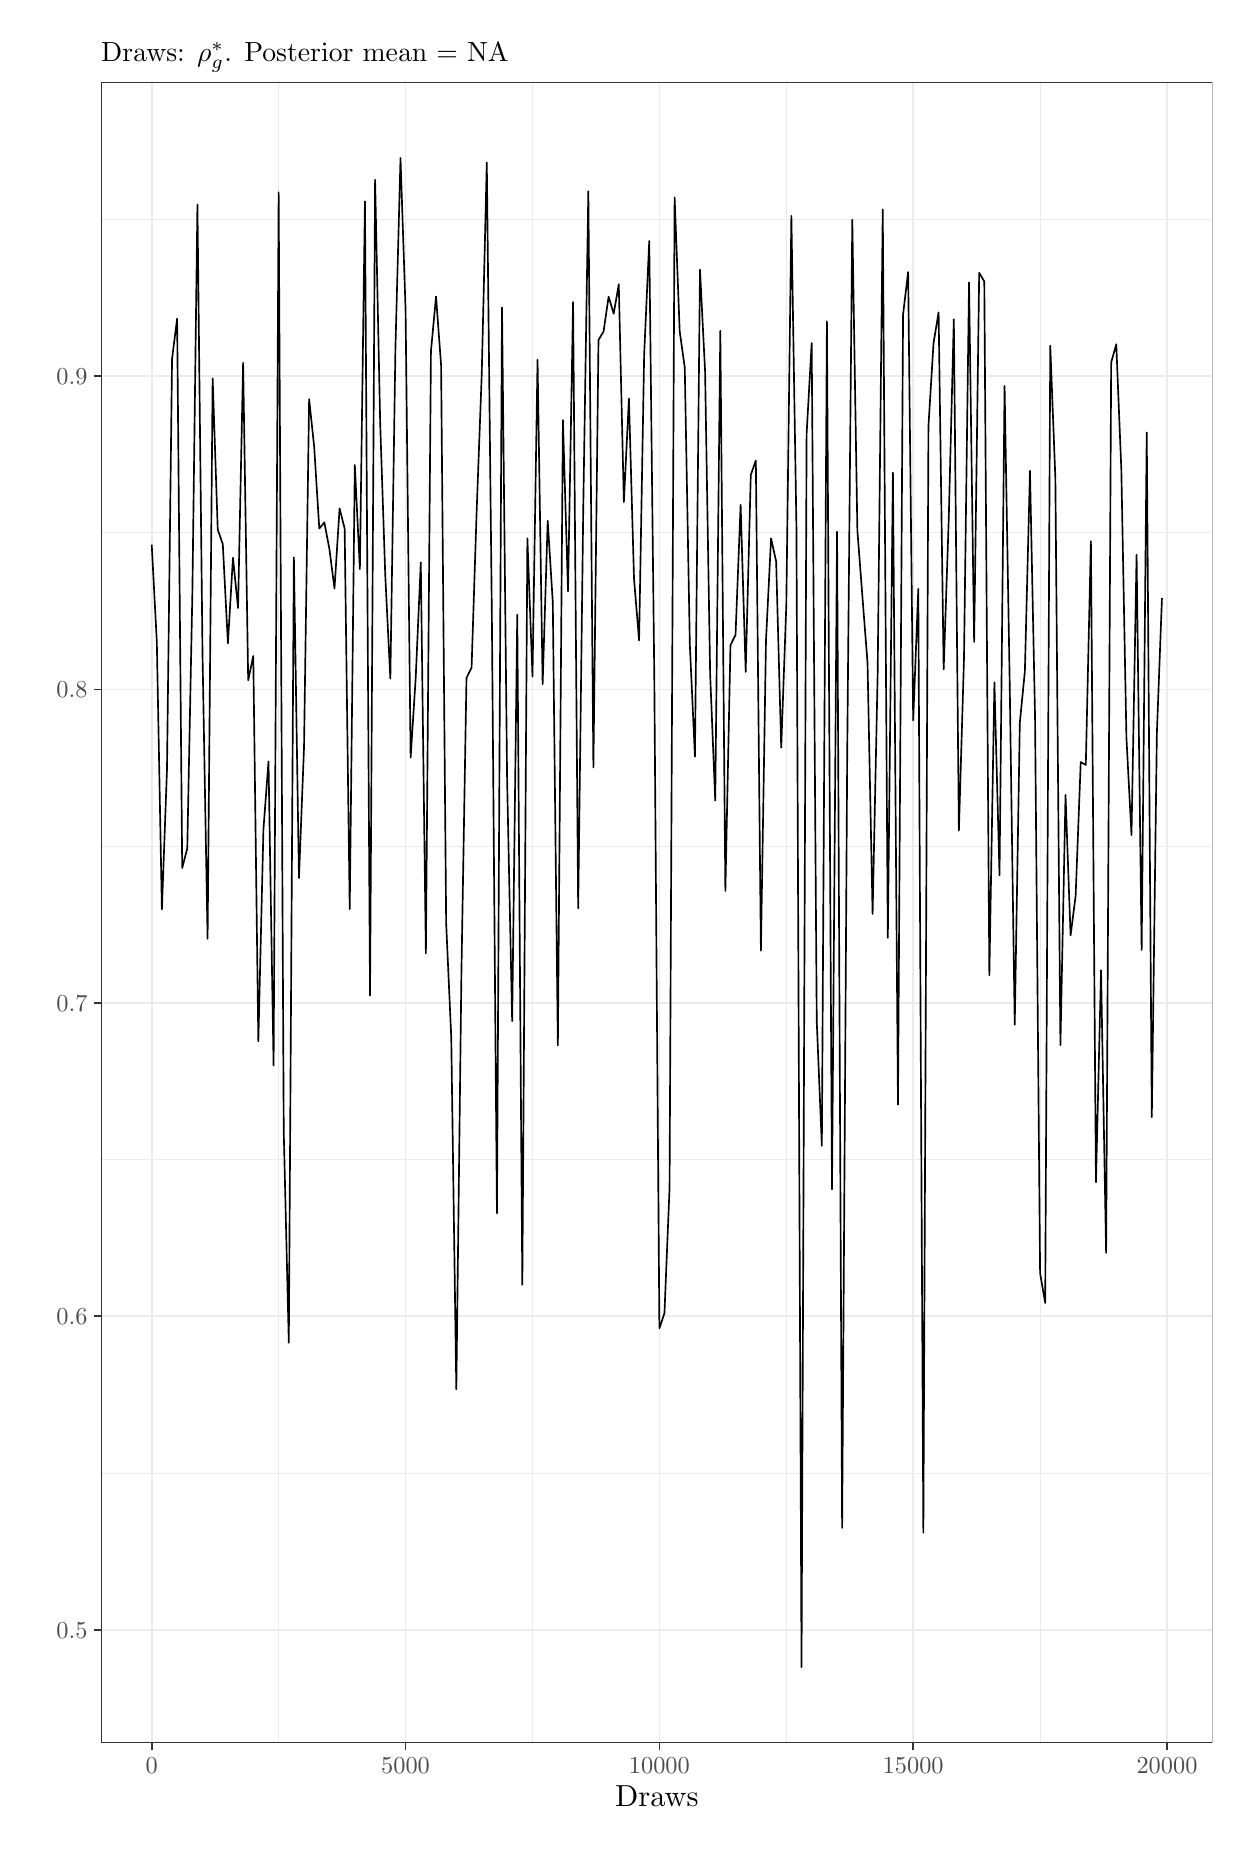
\begin{tikzpicture}[x=1pt,y=1pt]
\definecolor{fillColor}{RGB}{255,255,255}
\path[use as bounding box,fill=fillColor,fill opacity=0.00] (0,0) rectangle (433.62,650.43);
\begin{scope}
\path[clip] (  0.00,  0.00) rectangle (433.62,650.43);
\definecolor{drawColor}{RGB}{255,255,255}
\definecolor{fillColor}{RGB}{255,255,255}

\path[draw=drawColor,line width= 0.6pt,line join=round,line cap=round,fill=fillColor] (  0.00,  0.00) rectangle (433.62,650.43);
\end{scope}
\begin{scope}
\path[clip] ( 26.58, 30.69) rectangle (428.12,630.60);
\definecolor{fillColor}{RGB}{255,255,255}

\path[fill=fillColor] ( 26.58, 30.69) rectangle (428.12,630.60);
\definecolor{drawColor}{gray}{0.92}

\path[draw=drawColor,line width= 0.3pt,line join=round] ( 26.58,128.16) --
	(428.12,128.16);

\path[draw=drawColor,line width= 0.3pt,line join=round] ( 26.58,241.41) --
	(428.12,241.41);

\path[draw=drawColor,line width= 0.3pt,line join=round] ( 26.58,354.65) --
	(428.12,354.65);

\path[draw=drawColor,line width= 0.3pt,line join=round] ( 26.58,467.90) --
	(428.12,467.90);

\path[draw=drawColor,line width= 0.3pt,line join=round] ( 26.58,581.15) --
	(428.12,581.15);

\path[draw=drawColor,line width= 0.3pt,line join=round] ( 90.69, 30.69) --
	( 90.69,630.60);

\path[draw=drawColor,line width= 0.3pt,line join=round] (182.41, 30.69) --
	(182.41,630.60);

\path[draw=drawColor,line width= 0.3pt,line join=round] (274.13, 30.69) --
	(274.13,630.60);

\path[draw=drawColor,line width= 0.3pt,line join=round] (365.84, 30.69) --
	(365.84,630.60);

\path[draw=drawColor,line width= 0.6pt,line join=round] ( 26.58, 71.54) --
	(428.12, 71.54);

\path[draw=drawColor,line width= 0.6pt,line join=round] ( 26.58,184.79) --
	(428.12,184.79);

\path[draw=drawColor,line width= 0.6pt,line join=round] ( 26.58,298.03) --
	(428.12,298.03);

\path[draw=drawColor,line width= 0.6pt,line join=round] ( 26.58,411.28) --
	(428.12,411.28);

\path[draw=drawColor,line width= 0.6pt,line join=round] ( 26.58,524.52) --
	(428.12,524.52);

\path[draw=drawColor,line width= 0.6pt,line join=round] ( 44.83, 30.69) --
	( 44.83,630.60);

\path[draw=drawColor,line width= 0.6pt,line join=round] (136.55, 30.69) --
	(136.55,630.60);

\path[draw=drawColor,line width= 0.6pt,line join=round] (228.27, 30.69) --
	(228.27,630.60);

\path[draw=drawColor,line width= 0.6pt,line join=round] (319.98, 30.69) --
	(319.98,630.60);

\path[draw=drawColor,line width= 0.6pt,line join=round] (411.70, 30.69) --
	(411.70,630.60);
\definecolor{drawColor}{RGB}{0,0,0}

\path[draw=drawColor,line width= 0.6pt,line join=round] ( 44.83,463.59) --
	( 46.67,428.37) --
	( 48.50,331.84) --
	( 50.34,382.39) --
	( 52.17,530.69) --
	( 54.00,545.31) --
	( 55.84,346.78) --
	( 57.67,353.85) --
	( 59.51,446.02) --
	( 61.34,586.54) --
	( 63.18,423.93) --
	( 65.01,321.20) --
	( 66.84,523.73) --
	( 68.68,469.08) --
	( 70.51,463.77) --
	( 72.35,427.96) --
	( 74.18,458.88) --
	( 76.02,440.71) --
	( 77.85,529.30) --
	( 79.68,414.62) --
	( 81.52,423.39) --
	( 83.35,284.11) --
	( 85.19,360.72) --
	( 87.02,385.30) --
	( 88.86,275.40) --
	( 90.69,590.93) --
	( 92.53,251.55) --
	( 94.36,175.19) --
	( 96.19,459.07) --
	( 98.03,343.15) --
	( 99.86,390.52) --
	(101.70,516.22) --
	(103.53,498.94) --
	(105.37,469.45) --
	(107.20,471.65) --
	(109.03,462.04) --
	(110.87,447.74) --
	(112.70,476.73) --
	(114.54,469.39) --
	(116.37,331.90) --
	(118.21,492.39) --
	(120.04,454.76) --
	(121.87,587.66) --
	(123.71,300.66) --
	(125.54,595.48) --
	(127.38,507.41) --
	(129.21,452.62) --
	(131.05,415.22) --
	(132.88,534.30) --
	(134.72,603.33) --
	(136.55,548.60) --
	(138.38,386.65) --
	(140.22,415.59) --
	(142.05,457.21) --
	(143.89,315.90) --
	(145.72,533.48) --
	(147.56,553.26) --
	(149.39,528.40) --
	(151.22,326.80) --
	(153.06,285.59) --
	(154.89,158.39) --
	(156.73,308.89) --
	(158.56,415.45) --
	(160.40,419.20) --
	(162.23,475.51) --
	(164.06,524.78) --
	(165.90,601.71) --
	(167.73,438.20) --
	(169.57,221.98) --
	(171.40,549.29) --
	(173.24,378.87) --
	(175.07,291.44) --
	(176.91,438.26) --
	(178.74,196.17) --
	(180.57,465.86) --
	(182.41,415.97) --
	(184.24,530.46) --
	(186.08,413.22) --
	(187.91,472.20) --
	(189.75,442.79) --
	(191.58,282.66) --
	(193.41,508.63) --
	(195.25,446.73) --
	(197.08,551.25) --
	(198.92,332.21) --
	(200.75,476.23) --
	(202.59,591.31) --
	(204.42,383.08) --
	(206.26,537.58) --
	(208.09,540.62) --
	(209.92,553.20) --
	(211.76,547.06) --
	(213.59,557.70) --
	(215.43,479.00) --
	(217.26,516.41) --
	(219.10,451.31) --
	(220.93,429.01) --
	(222.76,532.12) --
	(224.60,573.35) --
	(226.43,415.71) --
	(228.27,180.46) --
	(230.10,185.93) --
	(231.94,231.14) --
	(233.77,589.09) --
	(235.60,540.78) --
	(237.44,527.55) --
	(239.27,427.52) --
	(241.11,387.02) --
	(242.94,562.96) --
	(244.78,526.23) --
	(246.61,416.77) --
	(248.45,371.11) --
	(250.28,540.87) --
	(252.11,338.45) --
	(253.95,427.28) --
	(255.78,430.97) --
	(257.62,477.97) --
	(259.45,417.62) --
	(261.29,488.78) --
	(263.12,494.01) --
	(264.95,316.90) --
	(266.79,429.06) --
	(268.62,465.86) --
	(270.46,457.55) --
	(272.29,390.25) --
	(274.13,441.83) --
	(275.96,582.42) --
	(277.79,469.68) --
	(279.63, 57.95) --
	(281.46,503.56) --
	(283.30,536.46) --
	(285.13,291.41) --
	(286.97,246.39) --
	(288.80,544.33) --
	(290.64,230.64) --
	(292.47,468.28) --
	(294.30,108.31) --
	(296.14,388.24) --
	(297.97,581.03) --
	(299.81,468.69) --
	(301.64,444.72) --
	(303.48,420.86) --
	(305.31,330.17) --
	(307.14,416.96) --
	(308.98,584.76) --
	(310.81,321.51) --
	(312.65,489.66) --
	(314.48,261.26) --
	(316.32,546.81) --
	(318.15,562.12) --
	(319.98,400.11) --
	(321.82,447.65) --
	(323.65,106.63) --
	(325.49,506.45) --
	(327.32,536.38) --
	(329.16,547.56) --
	(330.99,418.51) --
	(332.83,472.99) --
	(334.66,545.06) --
	(336.49,360.28) --
	(338.33,422.33) --
	(340.16,558.34) --
	(342.00,428.50) --
	(343.83,561.86) --
	(345.67,558.72) --
	(347.50,308.01) --
	(349.33,413.84) --
	(351.17,344.16) --
	(353.00,520.96) --
	(354.84,414.36) --
	(356.67,290.09) --
	(358.51,399.24) --
	(360.34,417.94) --
	(362.18,490.29) --
	(364.01,401.49) --
	(365.84,200.30) --
	(367.68,189.61) --
	(369.51,535.50) --
	(371.35,487.65) --
	(373.18,282.78) --
	(375.02,373.15) --
	(376.85,322.42) --
	(378.68,336.74) --
	(380.52,385.08) --
	(382.35,383.99) --
	(384.19,464.86) --
	(386.02,233.18) --
	(387.86,309.83) --
	(389.69,207.67) --
	(391.52,529.45) --
	(393.36,536.03) --
	(395.19,490.71) --
	(397.03,393.89) --
	(398.86,358.64) --
	(400.70,459.94) --
	(402.53,317.13) --
	(404.37,504.19) --
	(406.20,256.73) --
	(408.03,395.41) --
	(409.87,444.33);
\definecolor{drawColor}{gray}{0.20}

\path[draw=drawColor,line width= 0.6pt,line join=round,line cap=round] ( 26.58, 30.69) rectangle (428.12,630.60);
\end{scope}
\begin{scope}
\path[clip] (  0.00,  0.00) rectangle (433.62,650.43);
\definecolor{drawColor}{gray}{0.30}

\node[text=drawColor,anchor=base east,inner sep=0pt, outer sep=0pt, scale=  0.88] at ( 21.63, 68.51) {0.5};

\node[text=drawColor,anchor=base east,inner sep=0pt, outer sep=0pt, scale=  0.88] at ( 21.63,181.76) {0.6};

\node[text=drawColor,anchor=base east,inner sep=0pt, outer sep=0pt, scale=  0.88] at ( 21.63,295.00) {0.7};

\node[text=drawColor,anchor=base east,inner sep=0pt, outer sep=0pt, scale=  0.88] at ( 21.63,408.25) {0.8};

\node[text=drawColor,anchor=base east,inner sep=0pt, outer sep=0pt, scale=  0.88] at ( 21.63,521.49) {0.9};
\end{scope}
\begin{scope}
\path[clip] (  0.00,  0.00) rectangle (433.62,650.43);
\definecolor{drawColor}{gray}{0.20}

\path[draw=drawColor,line width= 0.6pt,line join=round] ( 23.83, 71.54) --
	( 26.58, 71.54);

\path[draw=drawColor,line width= 0.6pt,line join=round] ( 23.83,184.79) --
	( 26.58,184.79);

\path[draw=drawColor,line width= 0.6pt,line join=round] ( 23.83,298.03) --
	( 26.58,298.03);

\path[draw=drawColor,line width= 0.6pt,line join=round] ( 23.83,411.28) --
	( 26.58,411.28);

\path[draw=drawColor,line width= 0.6pt,line join=round] ( 23.83,524.52) --
	( 26.58,524.52);
\end{scope}
\begin{scope}
\path[clip] (  0.00,  0.00) rectangle (433.62,650.43);
\definecolor{drawColor}{gray}{0.20}

\path[draw=drawColor,line width= 0.6pt,line join=round] ( 44.83, 27.94) --
	( 44.83, 30.69);

\path[draw=drawColor,line width= 0.6pt,line join=round] (136.55, 27.94) --
	(136.55, 30.69);

\path[draw=drawColor,line width= 0.6pt,line join=round] (228.27, 27.94) --
	(228.27, 30.69);

\path[draw=drawColor,line width= 0.6pt,line join=round] (319.98, 27.94) --
	(319.98, 30.69);

\path[draw=drawColor,line width= 0.6pt,line join=round] (411.70, 27.94) --
	(411.70, 30.69);
\end{scope}
\begin{scope}
\path[clip] (  0.00,  0.00) rectangle (433.62,650.43);
\definecolor{drawColor}{gray}{0.30}

\node[text=drawColor,anchor=base,inner sep=0pt, outer sep=0pt, scale=  0.88] at ( 44.83, 19.68) {0};

\node[text=drawColor,anchor=base,inner sep=0pt, outer sep=0pt, scale=  0.88] at (136.55, 19.68) {5000};

\node[text=drawColor,anchor=base,inner sep=0pt, outer sep=0pt, scale=  0.88] at (228.27, 19.68) {10000};

\node[text=drawColor,anchor=base,inner sep=0pt, outer sep=0pt, scale=  0.88] at (319.98, 19.68) {15000};

\node[text=drawColor,anchor=base,inner sep=0pt, outer sep=0pt, scale=  0.88] at (411.70, 19.68) {20000};
\end{scope}
\begin{scope}
\path[clip] (  0.00,  0.00) rectangle (433.62,650.43);
\definecolor{drawColor}{RGB}{0,0,0}

\node[text=drawColor,anchor=base,inner sep=0pt, outer sep=0pt, scale=  1.10] at (227.35,  7.64) {Draws};
\end{scope}
\begin{scope}
\path[clip] (  0.00,  0.00) rectangle (433.62,650.43);
\definecolor{drawColor}{RGB}{0,0,0}

\node[text=drawColor,anchor=base west,inner sep=0pt, outer sep=0pt, scale=  1.00] at ( 26.58,638.04) {Draws: $\rho_g^*$. Posterior mean = NA};
\end{scope}
\end{tikzpicture}
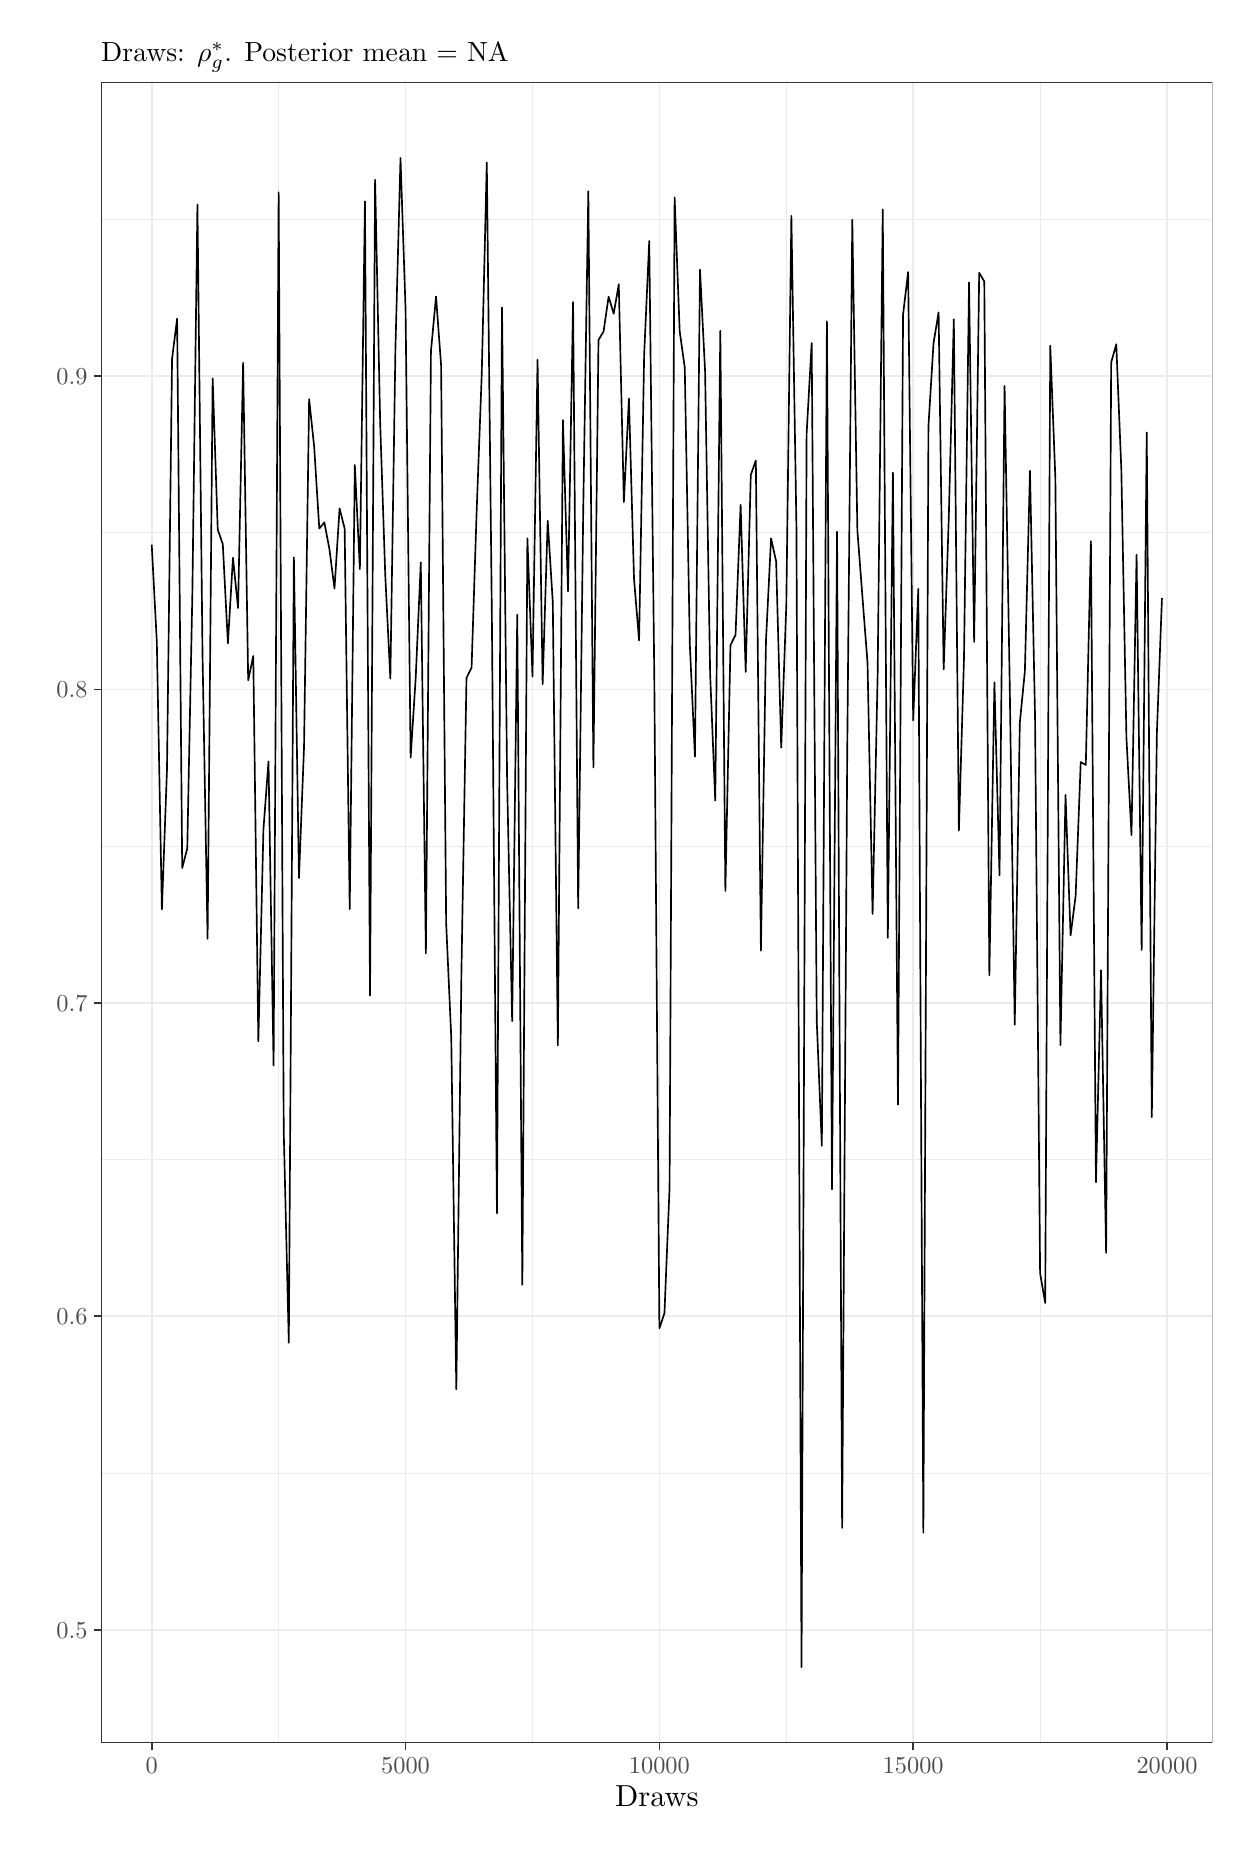
\begin{tikzpicture}[x=1pt,y=1pt]
\definecolor{fillColor}{RGB}{255,255,255}
\path[use as bounding box,fill=fillColor,fill opacity=0.00] (0,0) rectangle (433.62,650.43);
\begin{scope}
\path[clip] (  0.00,  0.00) rectangle (433.62,650.43);
\definecolor{drawColor}{RGB}{255,255,255}
\definecolor{fillColor}{RGB}{255,255,255}

\path[draw=drawColor,line width= 0.6pt,line join=round,line cap=round,fill=fillColor] (  0.00,  0.00) rectangle (433.62,650.43);
\end{scope}
\begin{scope}
\path[clip] ( 26.58, 30.69) rectangle (428.12,630.60);
\definecolor{fillColor}{RGB}{255,255,255}

\path[fill=fillColor] ( 26.58, 30.69) rectangle (428.12,630.60);
\definecolor{drawColor}{gray}{0.92}

\path[draw=drawColor,line width= 0.3pt,line join=round] ( 26.58,128.16) --
	(428.12,128.16);

\path[draw=drawColor,line width= 0.3pt,line join=round] ( 26.58,241.41) --
	(428.12,241.41);

\path[draw=drawColor,line width= 0.3pt,line join=round] ( 26.58,354.65) --
	(428.12,354.65);

\path[draw=drawColor,line width= 0.3pt,line join=round] ( 26.58,467.90) --
	(428.12,467.90);

\path[draw=drawColor,line width= 0.3pt,line join=round] ( 26.58,581.15) --
	(428.12,581.15);

\path[draw=drawColor,line width= 0.3pt,line join=round] ( 90.69, 30.69) --
	( 90.69,630.60);

\path[draw=drawColor,line width= 0.3pt,line join=round] (182.41, 30.69) --
	(182.41,630.60);

\path[draw=drawColor,line width= 0.3pt,line join=round] (274.13, 30.69) --
	(274.13,630.60);

\path[draw=drawColor,line width= 0.3pt,line join=round] (365.84, 30.69) --
	(365.84,630.60);

\path[draw=drawColor,line width= 0.6pt,line join=round] ( 26.58, 71.54) --
	(428.12, 71.54);

\path[draw=drawColor,line width= 0.6pt,line join=round] ( 26.58,184.79) --
	(428.12,184.79);

\path[draw=drawColor,line width= 0.6pt,line join=round] ( 26.58,298.03) --
	(428.12,298.03);

\path[draw=drawColor,line width= 0.6pt,line join=round] ( 26.58,411.28) --
	(428.12,411.28);

\path[draw=drawColor,line width= 0.6pt,line join=round] ( 26.58,524.52) --
	(428.12,524.52);

\path[draw=drawColor,line width= 0.6pt,line join=round] ( 44.83, 30.69) --
	( 44.83,630.60);

\path[draw=drawColor,line width= 0.6pt,line join=round] (136.55, 30.69) --
	(136.55,630.60);

\path[draw=drawColor,line width= 0.6pt,line join=round] (228.27, 30.69) --
	(228.27,630.60);

\path[draw=drawColor,line width= 0.6pt,line join=round] (319.98, 30.69) --
	(319.98,630.60);

\path[draw=drawColor,line width= 0.6pt,line join=round] (411.70, 30.69) --
	(411.70,630.60);
\definecolor{drawColor}{RGB}{0,0,0}

\path[draw=drawColor,line width= 0.6pt,line join=round] ( 44.83,463.59) --
	( 46.67,428.37) --
	( 48.50,331.84) --
	( 50.34,382.39) --
	( 52.17,530.69) --
	( 54.00,545.31) --
	( 55.84,346.78) --
	( 57.67,353.85) --
	( 59.51,446.02) --
	( 61.34,586.54) --
	( 63.18,423.93) --
	( 65.01,321.20) --
	( 66.84,523.73) --
	( 68.68,469.08) --
	( 70.51,463.77) --
	( 72.35,427.96) --
	( 74.18,458.88) --
	( 76.02,440.71) --
	( 77.85,529.30) --
	( 79.68,414.62) --
	( 81.52,423.39) --
	( 83.35,284.11) --
	( 85.19,360.72) --
	( 87.02,385.30) --
	( 88.86,275.40) --
	( 90.69,590.93) --
	( 92.53,251.55) --
	( 94.36,175.19) --
	( 96.19,459.07) --
	( 98.03,343.15) --
	( 99.86,390.52) --
	(101.70,516.22) --
	(103.53,498.94) --
	(105.37,469.45) --
	(107.20,471.65) --
	(109.03,462.04) --
	(110.87,447.74) --
	(112.70,476.73) --
	(114.54,469.39) --
	(116.37,331.90) --
	(118.21,492.39) --
	(120.04,454.76) --
	(121.87,587.66) --
	(123.71,300.66) --
	(125.54,595.48) --
	(127.38,507.41) --
	(129.21,452.62) --
	(131.05,415.22) --
	(132.88,534.30) --
	(134.72,603.33) --
	(136.55,548.60) --
	(138.38,386.65) --
	(140.22,415.59) --
	(142.05,457.21) --
	(143.89,315.90) --
	(145.72,533.48) --
	(147.56,553.26) --
	(149.39,528.40) --
	(151.22,326.80) --
	(153.06,285.59) --
	(154.89,158.39) --
	(156.73,308.89) --
	(158.56,415.45) --
	(160.40,419.20) --
	(162.23,475.51) --
	(164.06,524.78) --
	(165.90,601.71) --
	(167.73,438.20) --
	(169.57,221.98) --
	(171.40,549.29) --
	(173.24,378.87) --
	(175.07,291.44) --
	(176.91,438.26) --
	(178.74,196.17) --
	(180.57,465.86) --
	(182.41,415.97) --
	(184.24,530.46) --
	(186.08,413.22) --
	(187.91,472.20) --
	(189.75,442.79) --
	(191.58,282.66) --
	(193.41,508.63) --
	(195.25,446.73) --
	(197.08,551.25) --
	(198.92,332.21) --
	(200.75,476.23) --
	(202.59,591.31) --
	(204.42,383.08) --
	(206.26,537.58) --
	(208.09,540.62) --
	(209.92,553.20) --
	(211.76,547.06) --
	(213.59,557.70) --
	(215.43,479.00) --
	(217.26,516.41) --
	(219.10,451.31) --
	(220.93,429.01) --
	(222.76,532.12) --
	(224.60,573.35) --
	(226.43,415.71) --
	(228.27,180.46) --
	(230.10,185.93) --
	(231.94,231.14) --
	(233.77,589.09) --
	(235.60,540.78) --
	(237.44,527.55) --
	(239.27,427.52) --
	(241.11,387.02) --
	(242.94,562.96) --
	(244.78,526.23) --
	(246.61,416.77) --
	(248.45,371.11) --
	(250.28,540.87) --
	(252.11,338.45) --
	(253.95,427.28) --
	(255.78,430.97) --
	(257.62,477.97) --
	(259.45,417.62) --
	(261.29,488.78) --
	(263.12,494.01) --
	(264.95,316.90) --
	(266.79,429.06) --
	(268.62,465.86) --
	(270.46,457.55) --
	(272.29,390.25) --
	(274.13,441.83) --
	(275.96,582.42) --
	(277.79,469.68) --
	(279.63, 57.95) --
	(281.46,503.56) --
	(283.30,536.46) --
	(285.13,291.41) --
	(286.97,246.39) --
	(288.80,544.33) --
	(290.64,230.64) --
	(292.47,468.28) --
	(294.30,108.31) --
	(296.14,388.24) --
	(297.97,581.03) --
	(299.81,468.69) --
	(301.64,444.72) --
	(303.48,420.86) --
	(305.31,330.17) --
	(307.14,416.96) --
	(308.98,584.76) --
	(310.81,321.51) --
	(312.65,489.66) --
	(314.48,261.26) --
	(316.32,546.81) --
	(318.15,562.12) --
	(319.98,400.11) --
	(321.82,447.65) --
	(323.65,106.63) --
	(325.49,506.45) --
	(327.32,536.38) --
	(329.16,547.56) --
	(330.99,418.51) --
	(332.83,472.99) --
	(334.66,545.06) --
	(336.49,360.28) --
	(338.33,422.33) --
	(340.16,558.34) --
	(342.00,428.50) --
	(343.83,561.86) --
	(345.67,558.72) --
	(347.50,308.01) --
	(349.33,413.84) --
	(351.17,344.16) --
	(353.00,520.96) --
	(354.84,414.36) --
	(356.67,290.09) --
	(358.51,399.24) --
	(360.34,417.94) --
	(362.18,490.29) --
	(364.01,401.49) --
	(365.84,200.30) --
	(367.68,189.61) --
	(369.51,535.50) --
	(371.35,487.65) --
	(373.18,282.78) --
	(375.02,373.15) --
	(376.85,322.42) --
	(378.68,336.74) --
	(380.52,385.08) --
	(382.35,383.99) --
	(384.19,464.86) --
	(386.02,233.18) --
	(387.86,309.83) --
	(389.69,207.67) --
	(391.52,529.45) --
	(393.36,536.03) --
	(395.19,490.71) --
	(397.03,393.89) --
	(398.86,358.64) --
	(400.70,459.94) --
	(402.53,317.13) --
	(404.37,504.19) --
	(406.20,256.73) --
	(408.03,395.41) --
	(409.87,444.33);
\definecolor{drawColor}{gray}{0.20}

\path[draw=drawColor,line width= 0.6pt,line join=round,line cap=round] ( 26.58, 30.69) rectangle (428.12,630.60);
\end{scope}
\begin{scope}
\path[clip] (  0.00,  0.00) rectangle (433.62,650.43);
\definecolor{drawColor}{gray}{0.30}

\node[text=drawColor,anchor=base east,inner sep=0pt, outer sep=0pt, scale=  0.88] at ( 21.63, 68.51) {0.5};

\node[text=drawColor,anchor=base east,inner sep=0pt, outer sep=0pt, scale=  0.88] at ( 21.63,181.76) {0.6};

\node[text=drawColor,anchor=base east,inner sep=0pt, outer sep=0pt, scale=  0.88] at ( 21.63,295.00) {0.7};

\node[text=drawColor,anchor=base east,inner sep=0pt, outer sep=0pt, scale=  0.88] at ( 21.63,408.25) {0.8};

\node[text=drawColor,anchor=base east,inner sep=0pt, outer sep=0pt, scale=  0.88] at ( 21.63,521.49) {0.9};
\end{scope}
\begin{scope}
\path[clip] (  0.00,  0.00) rectangle (433.62,650.43);
\definecolor{drawColor}{gray}{0.20}

\path[draw=drawColor,line width= 0.6pt,line join=round] ( 23.83, 71.54) --
	( 26.58, 71.54);

\path[draw=drawColor,line width= 0.6pt,line join=round] ( 23.83,184.79) --
	( 26.58,184.79);

\path[draw=drawColor,line width= 0.6pt,line join=round] ( 23.83,298.03) --
	( 26.58,298.03);

\path[draw=drawColor,line width= 0.6pt,line join=round] ( 23.83,411.28) --
	( 26.58,411.28);

\path[draw=drawColor,line width= 0.6pt,line join=round] ( 23.83,524.52) --
	( 26.58,524.52);
\end{scope}
\begin{scope}
\path[clip] (  0.00,  0.00) rectangle (433.62,650.43);
\definecolor{drawColor}{gray}{0.20}

\path[draw=drawColor,line width= 0.6pt,line join=round] ( 44.83, 27.94) --
	( 44.83, 30.69);

\path[draw=drawColor,line width= 0.6pt,line join=round] (136.55, 27.94) --
	(136.55, 30.69);

\path[draw=drawColor,line width= 0.6pt,line join=round] (228.27, 27.94) --
	(228.27, 30.69);

\path[draw=drawColor,line width= 0.6pt,line join=round] (319.98, 27.94) --
	(319.98, 30.69);

\path[draw=drawColor,line width= 0.6pt,line join=round] (411.70, 27.94) --
	(411.70, 30.69);
\end{scope}
\begin{scope}
\path[clip] (  0.00,  0.00) rectangle (433.62,650.43);
\definecolor{drawColor}{gray}{0.30}

\node[text=drawColor,anchor=base,inner sep=0pt, outer sep=0pt, scale=  0.88] at ( 44.83, 19.68) {0};

\node[text=drawColor,anchor=base,inner sep=0pt, outer sep=0pt, scale=  0.88] at (136.55, 19.68) {5000};

\node[text=drawColor,anchor=base,inner sep=0pt, outer sep=0pt, scale=  0.88] at (228.27, 19.68) {10000};

\node[text=drawColor,anchor=base,inner sep=0pt, outer sep=0pt, scale=  0.88] at (319.98, 19.68) {15000};

\node[text=drawColor,anchor=base,inner sep=0pt, outer sep=0pt, scale=  0.88] at (411.70, 19.68) {20000};
\end{scope}
\begin{scope}
\path[clip] (  0.00,  0.00) rectangle (433.62,650.43);
\definecolor{drawColor}{RGB}{0,0,0}

\node[text=drawColor,anchor=base,inner sep=0pt, outer sep=0pt, scale=  1.10] at (227.35,  7.64) {Draws};
\end{scope}
\begin{scope}
\path[clip] (  0.00,  0.00) rectangle (433.62,650.43);
\definecolor{drawColor}{RGB}{0,0,0}

\node[text=drawColor,anchor=base west,inner sep=0pt, outer sep=0pt, scale=  1.00] at ( 26.58,638.04) {Draws: $\rho_g^*$. Posterior mean = NA};
\end{scope}
\end{tikzpicture}
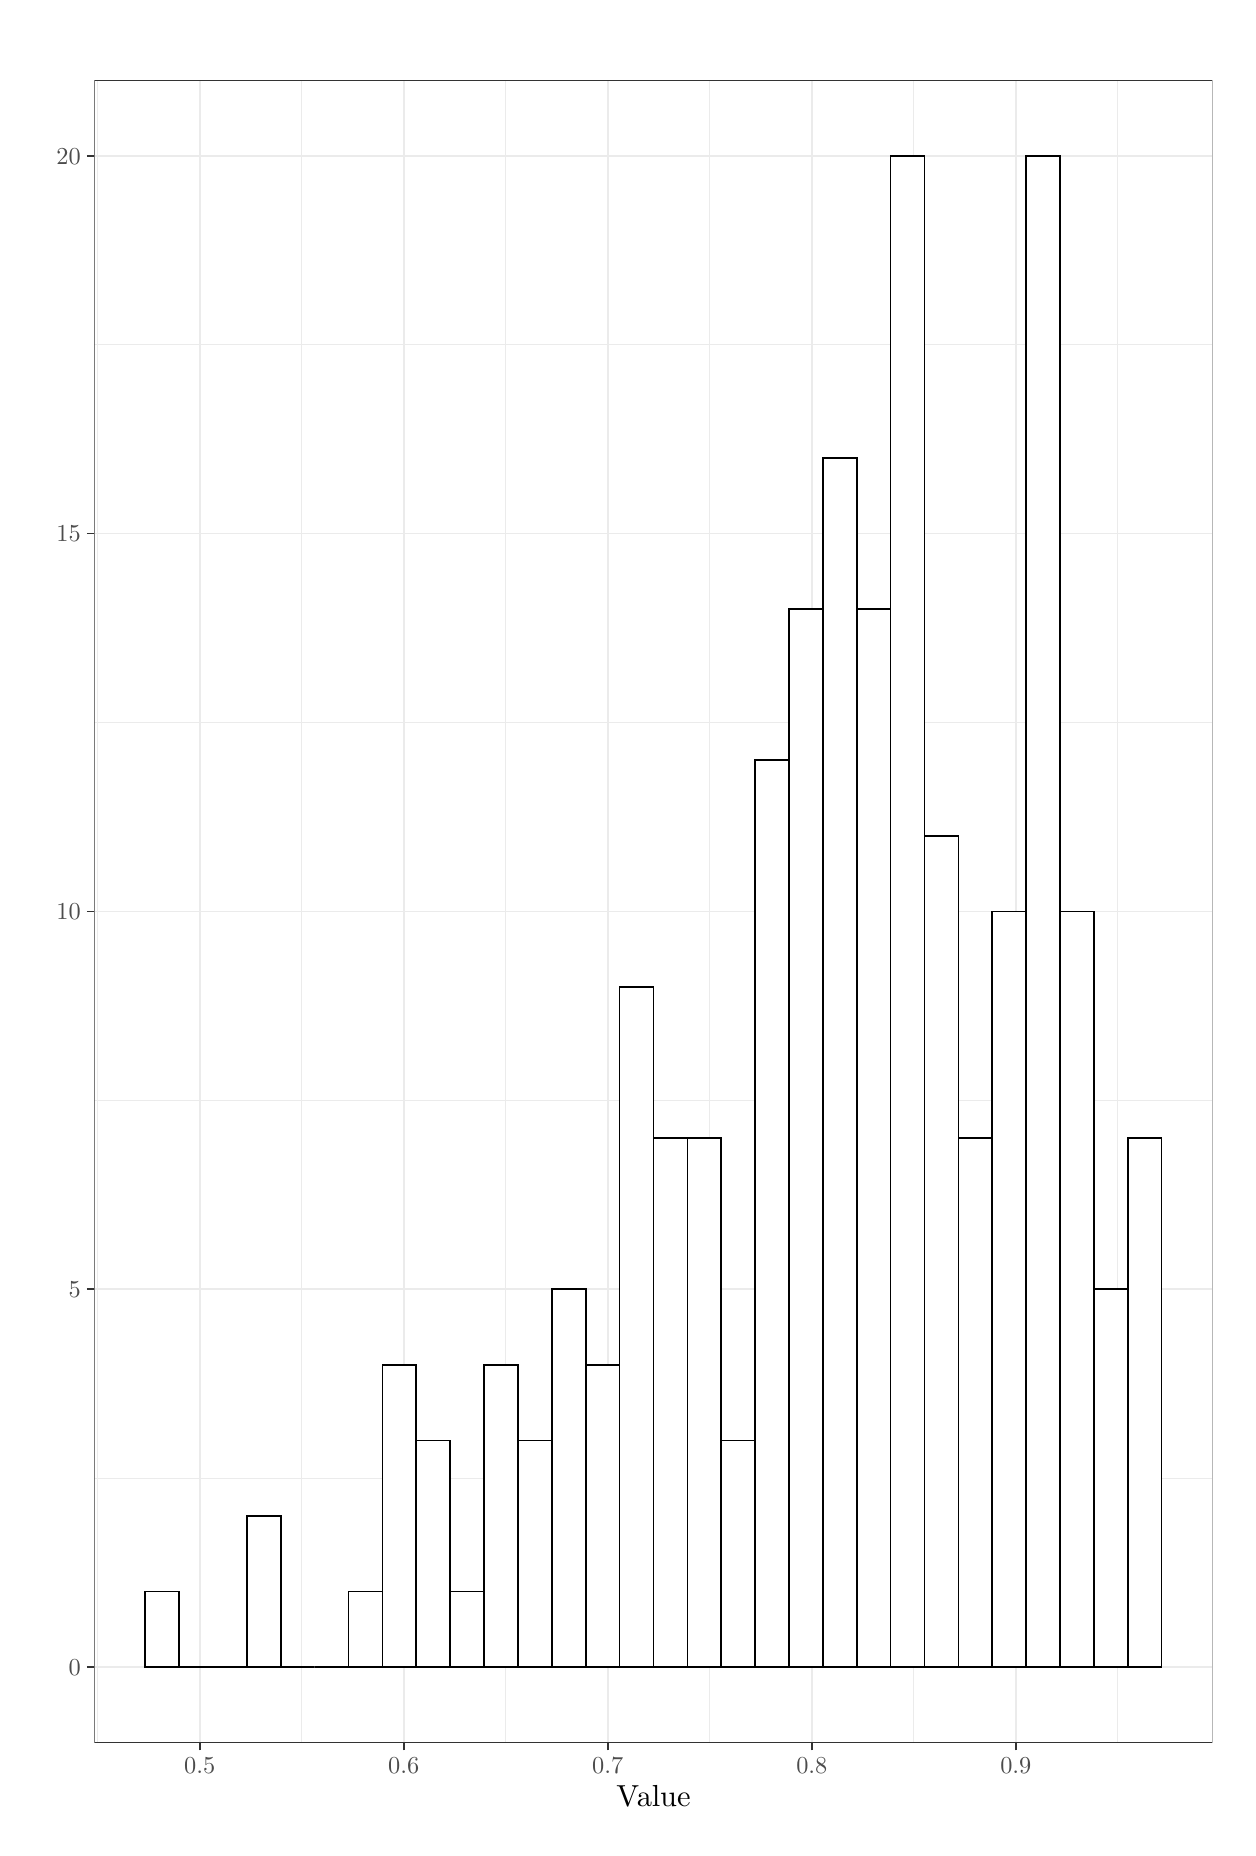
\begin{tikzpicture}[x=1pt,y=1pt]
\definecolor{fillColor}{RGB}{255,255,255}
\path[use as bounding box,fill=fillColor,fill opacity=0.00] (0,0) rectangle (433.62,650.43);
\begin{scope}
\path[clip] (  0.00,  0.00) rectangle (433.62,650.43);
\definecolor{drawColor}{RGB}{255,255,255}
\definecolor{fillColor}{RGB}{255,255,255}

\path[draw=drawColor,line width= 0.6pt,line join=round,line cap=round,fill=fillColor] (  0.00,  0.00) rectangle (433.62,650.43);
\end{scope}
\begin{scope}
\path[clip] ( 24.14, 30.69) rectangle (428.12,631.48);
\definecolor{fillColor}{RGB}{255,255,255}

\path[fill=fillColor] ( 24.14, 30.69) rectangle (428.12,631.48);
\definecolor{drawColor}{gray}{0.92}

\path[draw=drawColor,line width= 0.3pt,line join=round] ( 24.14,126.27) --
	(428.12,126.27);

\path[draw=drawColor,line width= 0.3pt,line join=round] ( 24.14,262.81) --
	(428.12,262.81);

\path[draw=drawColor,line width= 0.3pt,line join=round] ( 24.14,399.36) --
	(428.12,399.36);

\path[draw=drawColor,line width= 0.3pt,line join=round] ( 24.14,535.90) --
	(428.12,535.90);

\path[draw=drawColor,line width= 0.3pt,line join=round] ( 25.34, 30.69) --
	( 25.34,631.48);

\path[draw=drawColor,line width= 0.3pt,line join=round] ( 99.05, 30.69) --
	( 99.05,631.48);

\path[draw=drawColor,line width= 0.3pt,line join=round] (172.77, 30.69) --
	(172.77,631.48);

\path[draw=drawColor,line width= 0.3pt,line join=round] (246.49, 30.69) --
	(246.49,631.48);

\path[draw=drawColor,line width= 0.3pt,line join=round] (320.21, 30.69) --
	(320.21,631.48);

\path[draw=drawColor,line width= 0.3pt,line join=round] (393.93, 30.69) --
	(393.93,631.48);

\path[draw=drawColor,line width= 0.6pt,line join=round] ( 24.14, 57.99) --
	(428.12, 57.99);

\path[draw=drawColor,line width= 0.6pt,line join=round] ( 24.14,194.54) --
	(428.12,194.54);

\path[draw=drawColor,line width= 0.6pt,line join=round] ( 24.14,331.08) --
	(428.12,331.08);

\path[draw=drawColor,line width= 0.6pt,line join=round] ( 24.14,467.63) --
	(428.12,467.63);

\path[draw=drawColor,line width= 0.6pt,line join=round] ( 24.14,604.17) --
	(428.12,604.17);

\path[draw=drawColor,line width= 0.6pt,line join=round] ( 62.19, 30.69) --
	( 62.19,631.48);

\path[draw=drawColor,line width= 0.6pt,line join=round] (135.91, 30.69) --
	(135.91,631.48);

\path[draw=drawColor,line width= 0.6pt,line join=round] (209.63, 30.69) --
	(209.63,631.48);

\path[draw=drawColor,line width= 0.6pt,line join=round] (283.35, 30.69) --
	(283.35,631.48);

\path[draw=drawColor,line width= 0.6pt,line join=round] (357.07, 30.69) --
	(357.07,631.48);
\definecolor{drawColor}{RGB}{0,0,0}

\path[draw=drawColor,line width= 0.6pt,fill=fillColor] ( 42.50, 57.99) rectangle ( 54.74, 85.30);

\path[draw=drawColor,line width= 0.6pt,fill=fillColor] ( 54.74, 57.99) rectangle ( 66.98, 57.99);

\path[draw=drawColor,line width= 0.6pt,fill=fillColor] ( 66.98, 57.99) rectangle ( 79.22, 57.99);

\path[draw=drawColor,line width= 0.6pt,fill=fillColor] ( 79.22, 57.99) rectangle ( 91.47,112.61);

\path[draw=drawColor,line width= 0.6pt,fill=fillColor] ( 91.47, 57.99) rectangle (103.71, 57.99);

\path[draw=drawColor,line width= 0.6pt,fill=fillColor] (103.71, 57.99) rectangle (115.95, 57.99);

\path[draw=drawColor,line width= 0.6pt,fill=fillColor] (115.95, 57.99) rectangle (128.19, 85.30);

\path[draw=drawColor,line width= 0.6pt,fill=fillColor] (128.19, 57.99) rectangle (140.43,167.23);

\path[draw=drawColor,line width= 0.6pt,fill=fillColor] (140.43, 57.99) rectangle (152.68,139.92);

\path[draw=drawColor,line width= 0.6pt,fill=fillColor] (152.68, 57.99) rectangle (164.92, 85.30);

\path[draw=drawColor,line width= 0.6pt,fill=fillColor] (164.92, 57.99) rectangle (177.16,167.23);

\path[draw=drawColor,line width= 0.6pt,fill=fillColor] (177.16, 57.99) rectangle (189.40,139.92);

\path[draw=drawColor,line width= 0.6pt,fill=fillColor] (189.40, 57.99) rectangle (201.64,194.54);

\path[draw=drawColor,line width= 0.6pt,fill=fillColor] (201.64, 57.99) rectangle (213.89,167.23);

\path[draw=drawColor,line width= 0.6pt,fill=fillColor] (213.89, 57.99) rectangle (226.13,303.77);

\path[draw=drawColor,line width= 0.6pt,fill=fillColor] (226.13, 57.99) rectangle (238.37,249.16);

\path[draw=drawColor,line width= 0.6pt,fill=fillColor] (238.37, 57.99) rectangle (250.61,249.16);

\path[draw=drawColor,line width= 0.6pt,fill=fillColor] (250.61, 57.99) rectangle (262.85,139.92);

\path[draw=drawColor,line width= 0.6pt,fill=fillColor] (262.85, 57.99) rectangle (275.10,385.70);

\path[draw=drawColor,line width= 0.6pt,fill=fillColor] (275.10, 57.99) rectangle (287.34,440.32);

\path[draw=drawColor,line width= 0.6pt,fill=fillColor] (287.34, 57.99) rectangle (299.58,494.94);

\path[draw=drawColor,line width= 0.6pt,fill=fillColor] (299.58, 57.99) rectangle (311.82,440.32);

\path[draw=drawColor,line width= 0.6pt,fill=fillColor] (311.82, 57.99) rectangle (324.06,604.17);

\path[draw=drawColor,line width= 0.6pt,fill=fillColor] (324.06, 57.99) rectangle (336.31,358.39);

\path[draw=drawColor,line width= 0.6pt,fill=fillColor] (336.31, 57.99) rectangle (348.55,249.16);

\path[draw=drawColor,line width= 0.6pt,fill=fillColor] (348.55, 57.99) rectangle (360.79,331.08);

\path[draw=drawColor,line width= 0.6pt,fill=fillColor] (360.79, 57.99) rectangle (373.03,604.17);

\path[draw=drawColor,line width= 0.6pt,fill=fillColor] (373.03, 57.99) rectangle (385.27,331.08);

\path[draw=drawColor,line width= 0.6pt,fill=fillColor] (385.27, 57.99) rectangle (397.52,194.54);

\path[draw=drawColor,line width= 0.6pt,fill=fillColor] (397.52, 57.99) rectangle (409.76,249.16);
\definecolor{drawColor}{gray}{0.20}

\path[draw=drawColor,line width= 0.6pt,line join=round,line cap=round] ( 24.14, 30.69) rectangle (428.12,631.48);
\end{scope}
\begin{scope}
\path[clip] (  0.00,  0.00) rectangle (433.62,650.43);
\definecolor{drawColor}{gray}{0.30}

\node[text=drawColor,anchor=base east,inner sep=0pt, outer sep=0pt, scale=  0.88] at ( 19.19, 54.96) {0};

\node[text=drawColor,anchor=base east,inner sep=0pt, outer sep=0pt, scale=  0.88] at ( 19.19,191.51) {5};

\node[text=drawColor,anchor=base east,inner sep=0pt, outer sep=0pt, scale=  0.88] at ( 19.19,328.05) {10};

\node[text=drawColor,anchor=base east,inner sep=0pt, outer sep=0pt, scale=  0.88] at ( 19.19,464.60) {15};

\node[text=drawColor,anchor=base east,inner sep=0pt, outer sep=0pt, scale=  0.88] at ( 19.19,601.14) {20};
\end{scope}
\begin{scope}
\path[clip] (  0.00,  0.00) rectangle (433.62,650.43);
\definecolor{drawColor}{gray}{0.20}

\path[draw=drawColor,line width= 0.6pt,line join=round] ( 21.39, 57.99) --
	( 24.14, 57.99);

\path[draw=drawColor,line width= 0.6pt,line join=round] ( 21.39,194.54) --
	( 24.14,194.54);

\path[draw=drawColor,line width= 0.6pt,line join=round] ( 21.39,331.08) --
	( 24.14,331.08);

\path[draw=drawColor,line width= 0.6pt,line join=round] ( 21.39,467.63) --
	( 24.14,467.63);

\path[draw=drawColor,line width= 0.6pt,line join=round] ( 21.39,604.17) --
	( 24.14,604.17);
\end{scope}
\begin{scope}
\path[clip] (  0.00,  0.00) rectangle (433.62,650.43);
\definecolor{drawColor}{gray}{0.20}

\path[draw=drawColor,line width= 0.6pt,line join=round] ( 62.19, 27.94) --
	( 62.19, 30.69);

\path[draw=drawColor,line width= 0.6pt,line join=round] (135.91, 27.94) --
	(135.91, 30.69);

\path[draw=drawColor,line width= 0.6pt,line join=round] (209.63, 27.94) --
	(209.63, 30.69);

\path[draw=drawColor,line width= 0.6pt,line join=round] (283.35, 27.94) --
	(283.35, 30.69);

\path[draw=drawColor,line width= 0.6pt,line join=round] (357.07, 27.94) --
	(357.07, 30.69);
\end{scope}
\begin{scope}
\path[clip] (  0.00,  0.00) rectangle (433.62,650.43);
\definecolor{drawColor}{gray}{0.30}

\node[text=drawColor,anchor=base,inner sep=0pt, outer sep=0pt, scale=  0.88] at ( 62.19, 19.68) {0.5};

\node[text=drawColor,anchor=base,inner sep=0pt, outer sep=0pt, scale=  0.88] at (135.91, 19.68) {0.6};

\node[text=drawColor,anchor=base,inner sep=0pt, outer sep=0pt, scale=  0.88] at (209.63, 19.68) {0.7};

\node[text=drawColor,anchor=base,inner sep=0pt, outer sep=0pt, scale=  0.88] at (283.35, 19.68) {0.8};

\node[text=drawColor,anchor=base,inner sep=0pt, outer sep=0pt, scale=  0.88] at (357.07, 19.68) {0.9};
\end{scope}
\begin{scope}
\path[clip] (  0.00,  0.00) rectangle (433.62,650.43);
\definecolor{drawColor}{RGB}{0,0,0}

\node[text=drawColor,anchor=base,inner sep=0pt, outer sep=0pt, scale=  1.10] at (226.13,  7.64) {Value};
\end{scope}
\end{tikzpicture}
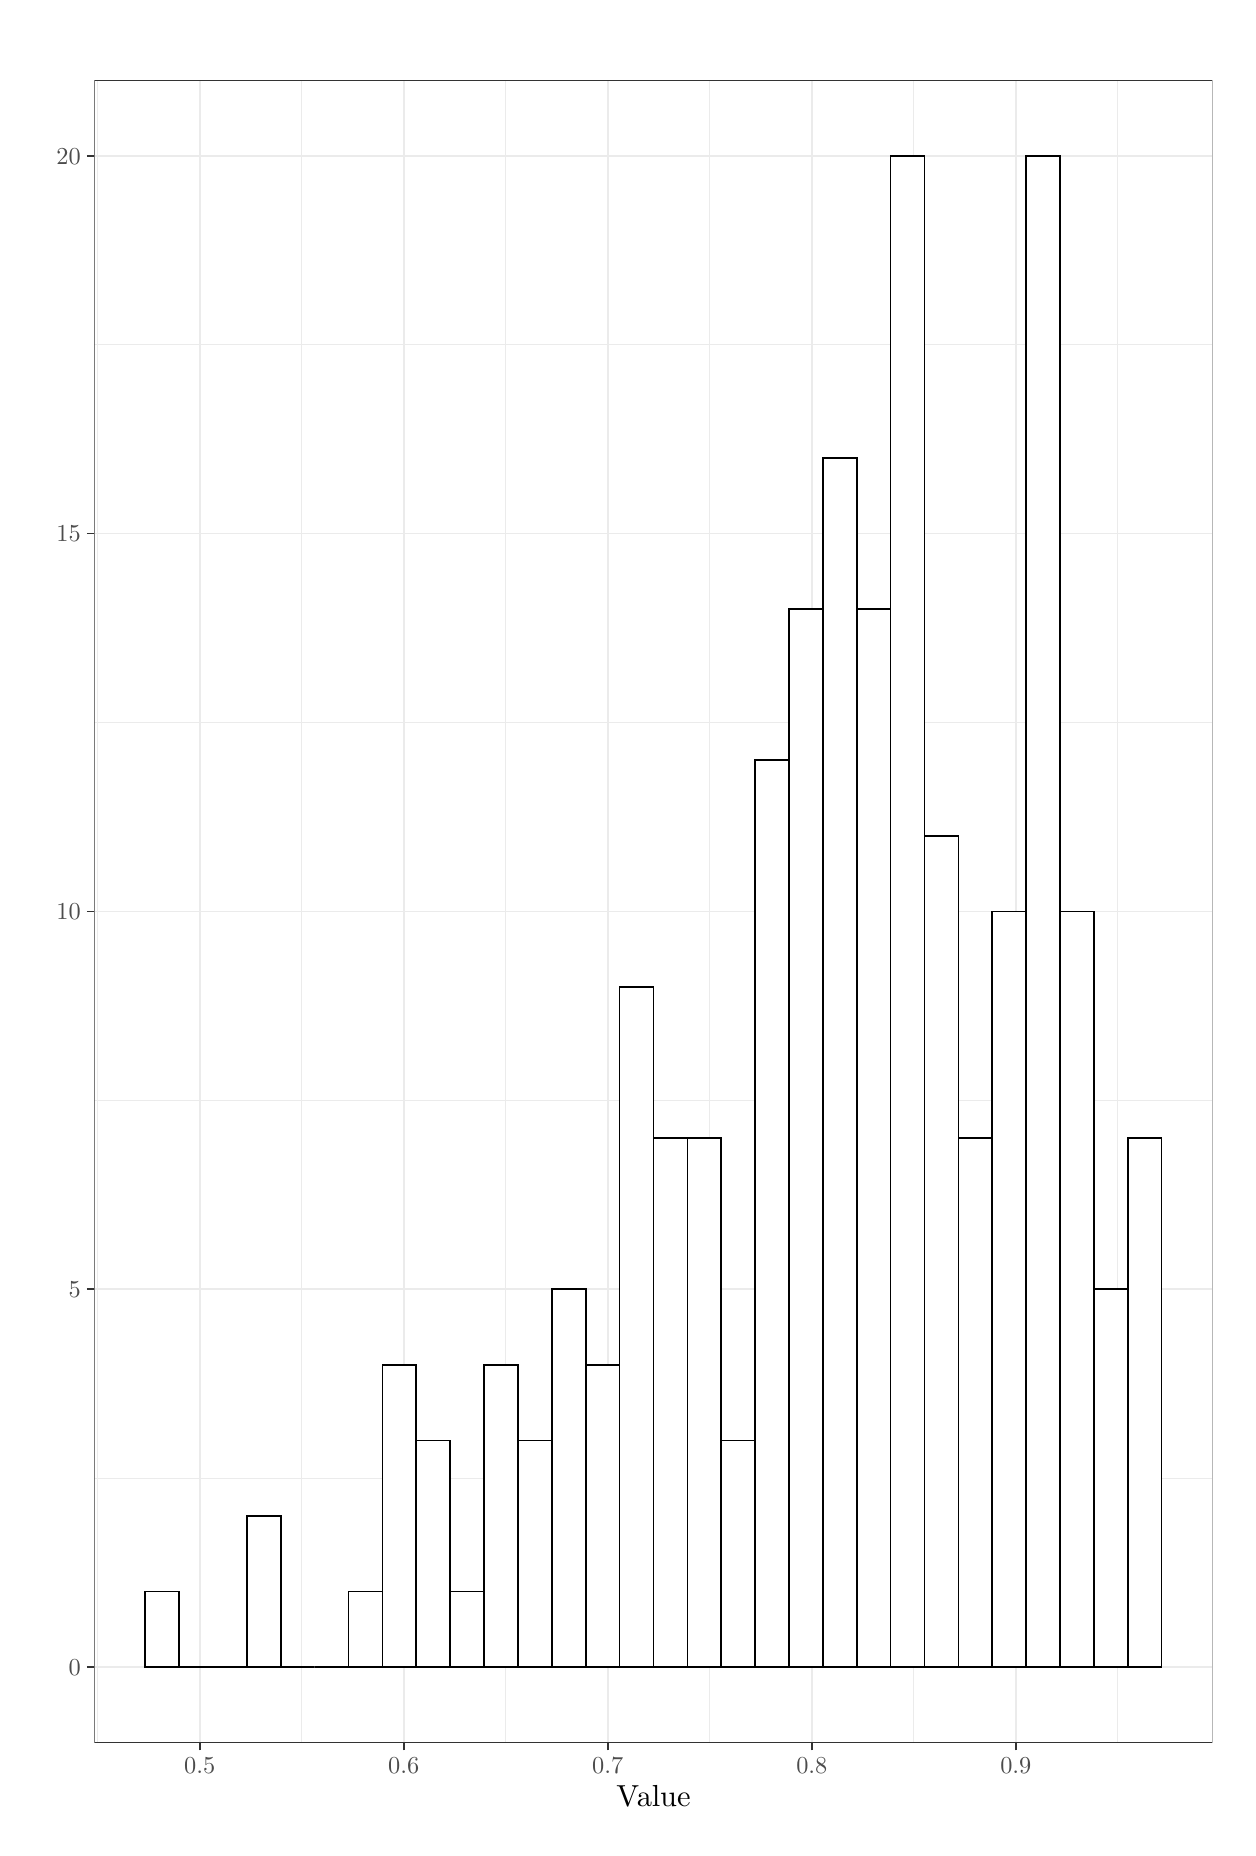
\begin{tikzpicture}[x=1pt,y=1pt]
\definecolor{fillColor}{RGB}{255,255,255}
\path[use as bounding box,fill=fillColor,fill opacity=0.00] (0,0) rectangle (433.62,650.43);
\begin{scope}
\path[clip] (  0.00,  0.00) rectangle (433.62,650.43);
\definecolor{drawColor}{RGB}{255,255,255}
\definecolor{fillColor}{RGB}{255,255,255}

\path[draw=drawColor,line width= 0.6pt,line join=round,line cap=round,fill=fillColor] (  0.00,  0.00) rectangle (433.62,650.43);
\end{scope}
\begin{scope}
\path[clip] ( 24.14, 30.69) rectangle (428.12,631.48);
\definecolor{fillColor}{RGB}{255,255,255}

\path[fill=fillColor] ( 24.14, 30.69) rectangle (428.12,631.48);
\definecolor{drawColor}{gray}{0.92}

\path[draw=drawColor,line width= 0.3pt,line join=round] ( 24.14,126.27) --
	(428.12,126.27);

\path[draw=drawColor,line width= 0.3pt,line join=round] ( 24.14,262.81) --
	(428.12,262.81);

\path[draw=drawColor,line width= 0.3pt,line join=round] ( 24.14,399.36) --
	(428.12,399.36);

\path[draw=drawColor,line width= 0.3pt,line join=round] ( 24.14,535.90) --
	(428.12,535.90);

\path[draw=drawColor,line width= 0.3pt,line join=round] ( 25.34, 30.69) --
	( 25.34,631.48);

\path[draw=drawColor,line width= 0.3pt,line join=round] ( 99.05, 30.69) --
	( 99.05,631.48);

\path[draw=drawColor,line width= 0.3pt,line join=round] (172.77, 30.69) --
	(172.77,631.48);

\path[draw=drawColor,line width= 0.3pt,line join=round] (246.49, 30.69) --
	(246.49,631.48);

\path[draw=drawColor,line width= 0.3pt,line join=round] (320.21, 30.69) --
	(320.21,631.48);

\path[draw=drawColor,line width= 0.3pt,line join=round] (393.93, 30.69) --
	(393.93,631.48);

\path[draw=drawColor,line width= 0.6pt,line join=round] ( 24.14, 57.99) --
	(428.12, 57.99);

\path[draw=drawColor,line width= 0.6pt,line join=round] ( 24.14,194.54) --
	(428.12,194.54);

\path[draw=drawColor,line width= 0.6pt,line join=round] ( 24.14,331.08) --
	(428.12,331.08);

\path[draw=drawColor,line width= 0.6pt,line join=round] ( 24.14,467.63) --
	(428.12,467.63);

\path[draw=drawColor,line width= 0.6pt,line join=round] ( 24.14,604.17) --
	(428.12,604.17);

\path[draw=drawColor,line width= 0.6pt,line join=round] ( 62.19, 30.69) --
	( 62.19,631.48);

\path[draw=drawColor,line width= 0.6pt,line join=round] (135.91, 30.69) --
	(135.91,631.48);

\path[draw=drawColor,line width= 0.6pt,line join=round] (209.63, 30.69) --
	(209.63,631.48);

\path[draw=drawColor,line width= 0.6pt,line join=round] (283.35, 30.69) --
	(283.35,631.48);

\path[draw=drawColor,line width= 0.6pt,line join=round] (357.07, 30.69) --
	(357.07,631.48);
\definecolor{drawColor}{RGB}{0,0,0}

\path[draw=drawColor,line width= 0.6pt,fill=fillColor] ( 42.50, 57.99) rectangle ( 54.74, 85.30);

\path[draw=drawColor,line width= 0.6pt,fill=fillColor] ( 54.74, 57.99) rectangle ( 66.98, 57.99);

\path[draw=drawColor,line width= 0.6pt,fill=fillColor] ( 66.98, 57.99) rectangle ( 79.22, 57.99);

\path[draw=drawColor,line width= 0.6pt,fill=fillColor] ( 79.22, 57.99) rectangle ( 91.47,112.61);

\path[draw=drawColor,line width= 0.6pt,fill=fillColor] ( 91.47, 57.99) rectangle (103.71, 57.99);

\path[draw=drawColor,line width= 0.6pt,fill=fillColor] (103.71, 57.99) rectangle (115.95, 57.99);

\path[draw=drawColor,line width= 0.6pt,fill=fillColor] (115.95, 57.99) rectangle (128.19, 85.30);

\path[draw=drawColor,line width= 0.6pt,fill=fillColor] (128.19, 57.99) rectangle (140.43,167.23);

\path[draw=drawColor,line width= 0.6pt,fill=fillColor] (140.43, 57.99) rectangle (152.68,139.92);

\path[draw=drawColor,line width= 0.6pt,fill=fillColor] (152.68, 57.99) rectangle (164.92, 85.30);

\path[draw=drawColor,line width= 0.6pt,fill=fillColor] (164.92, 57.99) rectangle (177.16,167.23);

\path[draw=drawColor,line width= 0.6pt,fill=fillColor] (177.16, 57.99) rectangle (189.40,139.92);

\path[draw=drawColor,line width= 0.6pt,fill=fillColor] (189.40, 57.99) rectangle (201.64,194.54);

\path[draw=drawColor,line width= 0.6pt,fill=fillColor] (201.64, 57.99) rectangle (213.89,167.23);

\path[draw=drawColor,line width= 0.6pt,fill=fillColor] (213.89, 57.99) rectangle (226.13,303.77);

\path[draw=drawColor,line width= 0.6pt,fill=fillColor] (226.13, 57.99) rectangle (238.37,249.16);

\path[draw=drawColor,line width= 0.6pt,fill=fillColor] (238.37, 57.99) rectangle (250.61,249.16);

\path[draw=drawColor,line width= 0.6pt,fill=fillColor] (250.61, 57.99) rectangle (262.85,139.92);

\path[draw=drawColor,line width= 0.6pt,fill=fillColor] (262.85, 57.99) rectangle (275.10,385.70);

\path[draw=drawColor,line width= 0.6pt,fill=fillColor] (275.10, 57.99) rectangle (287.34,440.32);

\path[draw=drawColor,line width= 0.6pt,fill=fillColor] (287.34, 57.99) rectangle (299.58,494.94);

\path[draw=drawColor,line width= 0.6pt,fill=fillColor] (299.58, 57.99) rectangle (311.82,440.32);

\path[draw=drawColor,line width= 0.6pt,fill=fillColor] (311.82, 57.99) rectangle (324.06,604.17);

\path[draw=drawColor,line width= 0.6pt,fill=fillColor] (324.06, 57.99) rectangle (336.31,358.39);

\path[draw=drawColor,line width= 0.6pt,fill=fillColor] (336.31, 57.99) rectangle (348.55,249.16);

\path[draw=drawColor,line width= 0.6pt,fill=fillColor] (348.55, 57.99) rectangle (360.79,331.08);

\path[draw=drawColor,line width= 0.6pt,fill=fillColor] (360.79, 57.99) rectangle (373.03,604.17);

\path[draw=drawColor,line width= 0.6pt,fill=fillColor] (373.03, 57.99) rectangle (385.27,331.08);

\path[draw=drawColor,line width= 0.6pt,fill=fillColor] (385.27, 57.99) rectangle (397.52,194.54);

\path[draw=drawColor,line width= 0.6pt,fill=fillColor] (397.52, 57.99) rectangle (409.76,249.16);
\definecolor{drawColor}{gray}{0.20}

\path[draw=drawColor,line width= 0.6pt,line join=round,line cap=round] ( 24.14, 30.69) rectangle (428.12,631.48);
\end{scope}
\begin{scope}
\path[clip] (  0.00,  0.00) rectangle (433.62,650.43);
\definecolor{drawColor}{gray}{0.30}

\node[text=drawColor,anchor=base east,inner sep=0pt, outer sep=0pt, scale=  0.88] at ( 19.19, 54.96) {0};

\node[text=drawColor,anchor=base east,inner sep=0pt, outer sep=0pt, scale=  0.88] at ( 19.19,191.51) {5};

\node[text=drawColor,anchor=base east,inner sep=0pt, outer sep=0pt, scale=  0.88] at ( 19.19,328.05) {10};

\node[text=drawColor,anchor=base east,inner sep=0pt, outer sep=0pt, scale=  0.88] at ( 19.19,464.60) {15};

\node[text=drawColor,anchor=base east,inner sep=0pt, outer sep=0pt, scale=  0.88] at ( 19.19,601.14) {20};
\end{scope}
\begin{scope}
\path[clip] (  0.00,  0.00) rectangle (433.62,650.43);
\definecolor{drawColor}{gray}{0.20}

\path[draw=drawColor,line width= 0.6pt,line join=round] ( 21.39, 57.99) --
	( 24.14, 57.99);

\path[draw=drawColor,line width= 0.6pt,line join=round] ( 21.39,194.54) --
	( 24.14,194.54);

\path[draw=drawColor,line width= 0.6pt,line join=round] ( 21.39,331.08) --
	( 24.14,331.08);

\path[draw=drawColor,line width= 0.6pt,line join=round] ( 21.39,467.63) --
	( 24.14,467.63);

\path[draw=drawColor,line width= 0.6pt,line join=round] ( 21.39,604.17) --
	( 24.14,604.17);
\end{scope}
\begin{scope}
\path[clip] (  0.00,  0.00) rectangle (433.62,650.43);
\definecolor{drawColor}{gray}{0.20}

\path[draw=drawColor,line width= 0.6pt,line join=round] ( 62.19, 27.94) --
	( 62.19, 30.69);

\path[draw=drawColor,line width= 0.6pt,line join=round] (135.91, 27.94) --
	(135.91, 30.69);

\path[draw=drawColor,line width= 0.6pt,line join=round] (209.63, 27.94) --
	(209.63, 30.69);

\path[draw=drawColor,line width= 0.6pt,line join=round] (283.35, 27.94) --
	(283.35, 30.69);

\path[draw=drawColor,line width= 0.6pt,line join=round] (357.07, 27.94) --
	(357.07, 30.69);
\end{scope}
\begin{scope}
\path[clip] (  0.00,  0.00) rectangle (433.62,650.43);
\definecolor{drawColor}{gray}{0.30}

\node[text=drawColor,anchor=base,inner sep=0pt, outer sep=0pt, scale=  0.88] at ( 62.19, 19.68) {0.5};

\node[text=drawColor,anchor=base,inner sep=0pt, outer sep=0pt, scale=  0.88] at (135.91, 19.68) {0.6};

\node[text=drawColor,anchor=base,inner sep=0pt, outer sep=0pt, scale=  0.88] at (209.63, 19.68) {0.7};

\node[text=drawColor,anchor=base,inner sep=0pt, outer sep=0pt, scale=  0.88] at (283.35, 19.68) {0.8};

\node[text=drawColor,anchor=base,inner sep=0pt, outer sep=0pt, scale=  0.88] at (357.07, 19.68) {0.9};
\end{scope}
\begin{scope}
\path[clip] (  0.00,  0.00) rectangle (433.62,650.43);
\definecolor{drawColor}{RGB}{0,0,0}

\node[text=drawColor,anchor=base,inner sep=0pt, outer sep=0pt, scale=  1.10] at (226.13,  7.64) {Value};
\end{scope}
\end{tikzpicture}
\begin{tikzpicture}[x=1pt,y=1pt]
\definecolor{fillColor}{RGB}{255,255,255}
\path[use as bounding box,fill=fillColor,fill opacity=0.00] (0,0) rectangle (433.62,650.43);
\begin{scope}
\path[clip] (  0.00,  0.00) rectangle (433.62,650.43);
\definecolor{drawColor}{RGB}{255,255,255}
\definecolor{fillColor}{RGB}{255,255,255}

\path[draw=drawColor,line width= 0.6pt,line join=round,line cap=round,fill=fillColor] (  0.00,  0.00) rectangle (433.62,650.43);
\end{scope}
\begin{scope}
\path[clip] ( 24.14, 30.69) rectangle (428.12,631.48);
\definecolor{fillColor}{RGB}{255,255,255}

\path[fill=fillColor] ( 24.14, 30.69) rectangle (428.12,631.48);
\definecolor{drawColor}{gray}{0.92}

\path[draw=drawColor,line width= 0.3pt,line join=round] ( 24.14,139.51) --
	(428.12,139.51);

\path[draw=drawColor,line width= 0.3pt,line join=round] ( 24.14,302.55) --
	(428.12,302.55);

\path[draw=drawColor,line width= 0.3pt,line join=round] ( 24.14,465.59) --
	(428.12,465.59);

\path[draw=drawColor,line width= 0.3pt,line join=round] ( 24.14,628.63) --
	(428.12,628.63);

\path[draw=drawColor,line width= 0.3pt,line join=round] ( 45.83, 30.69) --
	( 45.83,631.48);

\path[draw=drawColor,line width= 0.3pt,line join=round] (187.16, 30.69) --
	(187.16,631.48);

\path[draw=drawColor,line width= 0.3pt,line join=round] (328.49, 30.69) --
	(328.49,631.48);

\path[draw=drawColor,line width= 0.6pt,line join=round] ( 24.14, 57.99) --
	(428.12, 57.99);

\path[draw=drawColor,line width= 0.6pt,line join=round] ( 24.14,221.03) --
	(428.12,221.03);

\path[draw=drawColor,line width= 0.6pt,line join=round] ( 24.14,384.07) --
	(428.12,384.07);

\path[draw=drawColor,line width= 0.6pt,line join=round] ( 24.14,547.11) --
	(428.12,547.11);

\path[draw=drawColor,line width= 0.6pt,line join=round] (116.50, 30.69) --
	(116.50,631.48);

\path[draw=drawColor,line width= 0.6pt,line join=round] (257.82, 30.69) --
	(257.82,631.48);

\path[draw=drawColor,line width= 0.6pt,line join=round] (399.15, 30.69) --
	(399.15,631.48);
\definecolor{drawColor}{RGB}{0,0,0}

\path[draw=drawColor,line width= 0.6pt,fill=fillColor] ( 42.50, 57.99) rectangle ( 54.74, 82.45);

\path[draw=drawColor,line width= 0.6pt,fill=fillColor] ( 54.74, 57.99) rectangle ( 66.98,155.82);

\path[draw=drawColor,line width= 0.6pt,fill=fillColor] ( 66.98, 57.99) rectangle ( 79.22,294.40);

\path[draw=drawColor,line width= 0.6pt,fill=fillColor] ( 79.22, 57.99) rectangle ( 91.47,481.89);

\path[draw=drawColor,line width= 0.6pt,fill=fillColor] ( 91.47, 57.99) rectangle (103.71,604.17);

\path[draw=drawColor,line width= 0.6pt,fill=fillColor] (103.71, 57.99) rectangle (115.95,359.62);

\path[draw=drawColor,line width= 0.6pt,fill=fillColor] (115.95, 57.99) rectangle (128.19, 57.99);

\path[draw=drawColor,line width= 0.6pt,fill=fillColor] (128.19, 57.99) rectangle (140.43, 57.99);

\path[draw=drawColor,line width= 0.6pt,fill=fillColor] (140.43, 57.99) rectangle (152.68, 57.99);

\path[draw=drawColor,line width= 0.6pt,fill=fillColor] (152.68, 57.99) rectangle (164.92, 57.99);

\path[draw=drawColor,line width= 0.6pt,fill=fillColor] (164.92, 57.99) rectangle (177.16, 57.99);

\path[draw=drawColor,line width= 0.6pt,fill=fillColor] (177.16, 57.99) rectangle (189.40, 57.99);

\path[draw=drawColor,line width= 0.6pt,fill=fillColor] (189.40, 57.99) rectangle (201.64, 57.99);

\path[draw=drawColor,line width= 0.6pt,fill=fillColor] (201.64, 57.99) rectangle (213.89, 57.99);

\path[draw=drawColor,line width= 0.6pt,fill=fillColor] (213.89, 57.99) rectangle (226.13, 57.99);

\path[draw=drawColor,line width= 0.6pt,fill=fillColor] (226.13, 57.99) rectangle (238.37, 57.99);

\path[draw=drawColor,line width= 0.6pt,fill=fillColor] (238.37, 57.99) rectangle (250.61, 57.99);

\path[draw=drawColor,line width= 0.6pt,fill=fillColor] (250.61, 57.99) rectangle (262.85, 57.99);

\path[draw=drawColor,line width= 0.6pt,fill=fillColor] (262.85, 57.99) rectangle (275.10, 57.99);

\path[draw=drawColor,line width= 0.6pt,fill=fillColor] (275.10, 57.99) rectangle (287.34, 57.99);

\path[draw=drawColor,line width= 0.6pt,fill=fillColor] (287.34, 57.99) rectangle (299.58, 57.99);

\path[draw=drawColor,line width= 0.6pt,fill=fillColor] (299.58, 57.99) rectangle (311.82, 57.99);

\path[draw=drawColor,line width= 0.6pt,fill=fillColor] (311.82, 57.99) rectangle (324.06, 57.99);

\path[draw=drawColor,line width= 0.6pt,fill=fillColor] (324.06, 57.99) rectangle (336.31, 57.99);

\path[draw=drawColor,line width= 0.6pt,fill=fillColor] (336.31, 57.99) rectangle (348.55, 57.99);

\path[draw=drawColor,line width= 0.6pt,fill=fillColor] (348.55, 57.99) rectangle (360.79, 57.99);

\path[draw=drawColor,line width= 0.6pt,fill=fillColor] (360.79, 57.99) rectangle (373.03, 57.99);

\path[draw=drawColor,line width= 0.6pt,fill=fillColor] (373.03, 57.99) rectangle (385.27, 57.99);

\path[draw=drawColor,line width= 0.6pt,fill=fillColor] (385.27, 57.99) rectangle (397.52, 57.99);

\path[draw=drawColor,line width= 0.6pt,fill=fillColor] (397.52, 57.99) rectangle (409.76, 57.99);
\definecolor{drawColor}{gray}{0.20}

\path[draw=drawColor,line width= 0.6pt,line join=round,line cap=round] ( 24.14, 30.69) rectangle (428.12,631.48);
\end{scope}
\begin{scope}
\path[clip] (  0.00,  0.00) rectangle (433.62,650.43);
\definecolor{drawColor}{gray}{0.30}

\node[text=drawColor,anchor=base east,inner sep=0pt, outer sep=0pt, scale=  0.88] at ( 19.19, 54.96) {0};

\node[text=drawColor,anchor=base east,inner sep=0pt, outer sep=0pt, scale=  0.88] at ( 19.19,218.00) {20};

\node[text=drawColor,anchor=base east,inner sep=0pt, outer sep=0pt, scale=  0.88] at ( 19.19,381.04) {40};

\node[text=drawColor,anchor=base east,inner sep=0pt, outer sep=0pt, scale=  0.88] at ( 19.19,544.08) {60};
\end{scope}
\begin{scope}
\path[clip] (  0.00,  0.00) rectangle (433.62,650.43);
\definecolor{drawColor}{gray}{0.20}

\path[draw=drawColor,line width= 0.6pt,line join=round] ( 21.39, 57.99) --
	( 24.14, 57.99);

\path[draw=drawColor,line width= 0.6pt,line join=round] ( 21.39,221.03) --
	( 24.14,221.03);

\path[draw=drawColor,line width= 0.6pt,line join=round] ( 21.39,384.07) --
	( 24.14,384.07);

\path[draw=drawColor,line width= 0.6pt,line join=round] ( 21.39,547.11) --
	( 24.14,547.11);
\end{scope}
\begin{scope}
\path[clip] (  0.00,  0.00) rectangle (433.62,650.43);
\definecolor{drawColor}{gray}{0.20}

\path[draw=drawColor,line width= 0.6pt,line join=round] (116.50, 27.94) --
	(116.50, 30.69);

\path[draw=drawColor,line width= 0.6pt,line join=round] (257.82, 27.94) --
	(257.82, 30.69);

\path[draw=drawColor,line width= 0.6pt,line join=round] (399.15, 27.94) --
	(399.15, 30.69);
\end{scope}
\begin{scope}
\path[clip] (  0.00,  0.00) rectangle (433.62,650.43);
\definecolor{drawColor}{gray}{0.30}

\node[text=drawColor,anchor=base,inner sep=0pt, outer sep=0pt, scale=  0.88] at (116.50, 19.68) {1};

\node[text=drawColor,anchor=base,inner sep=0pt, outer sep=0pt, scale=  0.88] at (257.82, 19.68) {2};

\node[text=drawColor,anchor=base,inner sep=0pt, outer sep=0pt, scale=  0.88] at (399.15, 19.68) {3};
\end{scope}
\begin{scope}
\path[clip] (  0.00,  0.00) rectangle (433.62,650.43);
\definecolor{drawColor}{RGB}{0,0,0}

\node[text=drawColor,anchor=base,inner sep=0pt, outer sep=0pt, scale=  1.10] at (226.13,  7.64) {Value};
\end{scope}
\end{tikzpicture}
\begin{tikzpicture}[x=1pt,y=1pt]
\definecolor{fillColor}{RGB}{255,255,255}
\path[use as bounding box,fill=fillColor,fill opacity=0.00] (0,0) rectangle (433.62,650.43);
\begin{scope}
\path[clip] (  0.00,  0.00) rectangle (433.62,650.43);
\definecolor{drawColor}{RGB}{255,255,255}
\definecolor{fillColor}{RGB}{255,255,255}

\path[draw=drawColor,line width= 0.6pt,line join=round,line cap=round,fill=fillColor] (  0.00,  0.00) rectangle (433.62,650.43);
\end{scope}
\begin{scope}
\path[clip] ( 24.14, 30.69) rectangle (428.12,631.48);
\definecolor{fillColor}{RGB}{255,255,255}

\path[fill=fillColor] ( 24.14, 30.69) rectangle (428.12,631.48);
\definecolor{drawColor}{gray}{0.92}

\path[draw=drawColor,line width= 0.3pt,line join=round] ( 24.14,139.51) --
	(428.12,139.51);

\path[draw=drawColor,line width= 0.3pt,line join=round] ( 24.14,302.55) --
	(428.12,302.55);

\path[draw=drawColor,line width= 0.3pt,line join=round] ( 24.14,465.59) --
	(428.12,465.59);

\path[draw=drawColor,line width= 0.3pt,line join=round] ( 24.14,628.63) --
	(428.12,628.63);

\path[draw=drawColor,line width= 0.3pt,line join=round] ( 45.83, 30.69) --
	( 45.83,631.48);

\path[draw=drawColor,line width= 0.3pt,line join=round] (187.16, 30.69) --
	(187.16,631.48);

\path[draw=drawColor,line width= 0.3pt,line join=round] (328.49, 30.69) --
	(328.49,631.48);

\path[draw=drawColor,line width= 0.6pt,line join=round] ( 24.14, 57.99) --
	(428.12, 57.99);

\path[draw=drawColor,line width= 0.6pt,line join=round] ( 24.14,221.03) --
	(428.12,221.03);

\path[draw=drawColor,line width= 0.6pt,line join=round] ( 24.14,384.07) --
	(428.12,384.07);

\path[draw=drawColor,line width= 0.6pt,line join=round] ( 24.14,547.11) --
	(428.12,547.11);

\path[draw=drawColor,line width= 0.6pt,line join=round] (116.50, 30.69) --
	(116.50,631.48);

\path[draw=drawColor,line width= 0.6pt,line join=round] (257.82, 30.69) --
	(257.82,631.48);

\path[draw=drawColor,line width= 0.6pt,line join=round] (399.15, 30.69) --
	(399.15,631.48);
\definecolor{drawColor}{RGB}{0,0,0}

\path[draw=drawColor,line width= 0.6pt,fill=fillColor] ( 42.50, 57.99) rectangle ( 54.74, 82.45);

\path[draw=drawColor,line width= 0.6pt,fill=fillColor] ( 54.74, 57.99) rectangle ( 66.98,155.82);

\path[draw=drawColor,line width= 0.6pt,fill=fillColor] ( 66.98, 57.99) rectangle ( 79.22,294.40);

\path[draw=drawColor,line width= 0.6pt,fill=fillColor] ( 79.22, 57.99) rectangle ( 91.47,481.89);

\path[draw=drawColor,line width= 0.6pt,fill=fillColor] ( 91.47, 57.99) rectangle (103.71,604.17);

\path[draw=drawColor,line width= 0.6pt,fill=fillColor] (103.71, 57.99) rectangle (115.95,359.62);

\path[draw=drawColor,line width= 0.6pt,fill=fillColor] (115.95, 57.99) rectangle (128.19, 57.99);

\path[draw=drawColor,line width= 0.6pt,fill=fillColor] (128.19, 57.99) rectangle (140.43, 57.99);

\path[draw=drawColor,line width= 0.6pt,fill=fillColor] (140.43, 57.99) rectangle (152.68, 57.99);

\path[draw=drawColor,line width= 0.6pt,fill=fillColor] (152.68, 57.99) rectangle (164.92, 57.99);

\path[draw=drawColor,line width= 0.6pt,fill=fillColor] (164.92, 57.99) rectangle (177.16, 57.99);

\path[draw=drawColor,line width= 0.6pt,fill=fillColor] (177.16, 57.99) rectangle (189.40, 57.99);

\path[draw=drawColor,line width= 0.6pt,fill=fillColor] (189.40, 57.99) rectangle (201.64, 57.99);

\path[draw=drawColor,line width= 0.6pt,fill=fillColor] (201.64, 57.99) rectangle (213.89, 57.99);

\path[draw=drawColor,line width= 0.6pt,fill=fillColor] (213.89, 57.99) rectangle (226.13, 57.99);

\path[draw=drawColor,line width= 0.6pt,fill=fillColor] (226.13, 57.99) rectangle (238.37, 57.99);

\path[draw=drawColor,line width= 0.6pt,fill=fillColor] (238.37, 57.99) rectangle (250.61, 57.99);

\path[draw=drawColor,line width= 0.6pt,fill=fillColor] (250.61, 57.99) rectangle (262.85, 57.99);

\path[draw=drawColor,line width= 0.6pt,fill=fillColor] (262.85, 57.99) rectangle (275.10, 57.99);

\path[draw=drawColor,line width= 0.6pt,fill=fillColor] (275.10, 57.99) rectangle (287.34, 57.99);

\path[draw=drawColor,line width= 0.6pt,fill=fillColor] (287.34, 57.99) rectangle (299.58, 57.99);

\path[draw=drawColor,line width= 0.6pt,fill=fillColor] (299.58, 57.99) rectangle (311.82, 57.99);

\path[draw=drawColor,line width= 0.6pt,fill=fillColor] (311.82, 57.99) rectangle (324.06, 57.99);

\path[draw=drawColor,line width= 0.6pt,fill=fillColor] (324.06, 57.99) rectangle (336.31, 57.99);

\path[draw=drawColor,line width= 0.6pt,fill=fillColor] (336.31, 57.99) rectangle (348.55, 57.99);

\path[draw=drawColor,line width= 0.6pt,fill=fillColor] (348.55, 57.99) rectangle (360.79, 57.99);

\path[draw=drawColor,line width= 0.6pt,fill=fillColor] (360.79, 57.99) rectangle (373.03, 57.99);

\path[draw=drawColor,line width= 0.6pt,fill=fillColor] (373.03, 57.99) rectangle (385.27, 57.99);

\path[draw=drawColor,line width= 0.6pt,fill=fillColor] (385.27, 57.99) rectangle (397.52, 57.99);

\path[draw=drawColor,line width= 0.6pt,fill=fillColor] (397.52, 57.99) rectangle (409.76, 57.99);
\definecolor{drawColor}{gray}{0.20}

\path[draw=drawColor,line width= 0.6pt,line join=round,line cap=round] ( 24.14, 30.69) rectangle (428.12,631.48);
\end{scope}
\begin{scope}
\path[clip] (  0.00,  0.00) rectangle (433.62,650.43);
\definecolor{drawColor}{gray}{0.30}

\node[text=drawColor,anchor=base east,inner sep=0pt, outer sep=0pt, scale=  0.88] at ( 19.19, 54.96) {0};

\node[text=drawColor,anchor=base east,inner sep=0pt, outer sep=0pt, scale=  0.88] at ( 19.19,218.00) {20};

\node[text=drawColor,anchor=base east,inner sep=0pt, outer sep=0pt, scale=  0.88] at ( 19.19,381.04) {40};

\node[text=drawColor,anchor=base east,inner sep=0pt, outer sep=0pt, scale=  0.88] at ( 19.19,544.08) {60};
\end{scope}
\begin{scope}
\path[clip] (  0.00,  0.00) rectangle (433.62,650.43);
\definecolor{drawColor}{gray}{0.20}

\path[draw=drawColor,line width= 0.6pt,line join=round] ( 21.39, 57.99) --
	( 24.14, 57.99);

\path[draw=drawColor,line width= 0.6pt,line join=round] ( 21.39,221.03) --
	( 24.14,221.03);

\path[draw=drawColor,line width= 0.6pt,line join=round] ( 21.39,384.07) --
	( 24.14,384.07);

\path[draw=drawColor,line width= 0.6pt,line join=round] ( 21.39,547.11) --
	( 24.14,547.11);
\end{scope}
\begin{scope}
\path[clip] (  0.00,  0.00) rectangle (433.62,650.43);
\definecolor{drawColor}{gray}{0.20}

\path[draw=drawColor,line width= 0.6pt,line join=round] (116.50, 27.94) --
	(116.50, 30.69);

\path[draw=drawColor,line width= 0.6pt,line join=round] (257.82, 27.94) --
	(257.82, 30.69);

\path[draw=drawColor,line width= 0.6pt,line join=round] (399.15, 27.94) --
	(399.15, 30.69);
\end{scope}
\begin{scope}
\path[clip] (  0.00,  0.00) rectangle (433.62,650.43);
\definecolor{drawColor}{gray}{0.30}

\node[text=drawColor,anchor=base,inner sep=0pt, outer sep=0pt, scale=  0.88] at (116.50, 19.68) {1};

\node[text=drawColor,anchor=base,inner sep=0pt, outer sep=0pt, scale=  0.88] at (257.82, 19.68) {2};

\node[text=drawColor,anchor=base,inner sep=0pt, outer sep=0pt, scale=  0.88] at (399.15, 19.68) {3};
\end{scope}
\begin{scope}
\path[clip] (  0.00,  0.00) rectangle (433.62,650.43);
\definecolor{drawColor}{RGB}{0,0,0}

\node[text=drawColor,anchor=base,inner sep=0pt, outer sep=0pt, scale=  1.10] at (226.13,  7.64) {Value};
\end{scope}
\end{tikzpicture}
\begin{tikzpicture}[x=1pt,y=1pt]
\definecolor{fillColor}{RGB}{255,255,255}
\path[use as bounding box,fill=fillColor,fill opacity=0.00] (0,0) rectangle (433.62,650.43);
\begin{scope}
\path[clip] (  0.00,  0.00) rectangle (433.62,650.43);
\definecolor{drawColor}{RGB}{255,255,255}
\definecolor{fillColor}{RGB}{255,255,255}

\path[draw=drawColor,line width= 0.6pt,line join=round,line cap=round,fill=fillColor] (  0.00,  0.00) rectangle (433.62,650.43);
\end{scope}
\begin{scope}
\path[clip] ( 24.14, 30.69) rectangle (428.12,631.48);
\definecolor{fillColor}{RGB}{255,255,255}

\path[fill=fillColor] ( 24.14, 30.69) rectangle (428.12,631.48);
\definecolor{drawColor}{gray}{0.92}

\path[draw=drawColor,line width= 0.3pt,line join=round] ( 24.14,139.51) --
	(428.12,139.51);

\path[draw=drawColor,line width= 0.3pt,line join=round] ( 24.14,302.55) --
	(428.12,302.55);

\path[draw=drawColor,line width= 0.3pt,line join=round] ( 24.14,465.59) --
	(428.12,465.59);

\path[draw=drawColor,line width= 0.3pt,line join=round] ( 24.14,628.63) --
	(428.12,628.63);

\path[draw=drawColor,line width= 0.3pt,line join=round] ( 45.83, 30.69) --
	( 45.83,631.48);

\path[draw=drawColor,line width= 0.3pt,line join=round] (187.16, 30.69) --
	(187.16,631.48);

\path[draw=drawColor,line width= 0.3pt,line join=round] (328.49, 30.69) --
	(328.49,631.48);

\path[draw=drawColor,line width= 0.6pt,line join=round] ( 24.14, 57.99) --
	(428.12, 57.99);

\path[draw=drawColor,line width= 0.6pt,line join=round] ( 24.14,221.03) --
	(428.12,221.03);

\path[draw=drawColor,line width= 0.6pt,line join=round] ( 24.14,384.07) --
	(428.12,384.07);

\path[draw=drawColor,line width= 0.6pt,line join=round] ( 24.14,547.11) --
	(428.12,547.11);

\path[draw=drawColor,line width= 0.6pt,line join=round] (116.50, 30.69) --
	(116.50,631.48);

\path[draw=drawColor,line width= 0.6pt,line join=round] (257.82, 30.69) --
	(257.82,631.48);

\path[draw=drawColor,line width= 0.6pt,line join=round] (399.15, 30.69) --
	(399.15,631.48);
\definecolor{drawColor}{RGB}{0,0,0}

\path[draw=drawColor,line width= 0.6pt,fill=fillColor] ( 42.50, 57.99) rectangle ( 54.74, 82.45);

\path[draw=drawColor,line width= 0.6pt,fill=fillColor] ( 54.74, 57.99) rectangle ( 66.98,155.82);

\path[draw=drawColor,line width= 0.6pt,fill=fillColor] ( 66.98, 57.99) rectangle ( 79.22,294.40);

\path[draw=drawColor,line width= 0.6pt,fill=fillColor] ( 79.22, 57.99) rectangle ( 91.47,481.89);

\path[draw=drawColor,line width= 0.6pt,fill=fillColor] ( 91.47, 57.99) rectangle (103.71,604.17);

\path[draw=drawColor,line width= 0.6pt,fill=fillColor] (103.71, 57.99) rectangle (115.95,359.62);

\path[draw=drawColor,line width= 0.6pt,fill=fillColor] (115.95, 57.99) rectangle (128.19, 57.99);

\path[draw=drawColor,line width= 0.6pt,fill=fillColor] (128.19, 57.99) rectangle (140.43, 57.99);

\path[draw=drawColor,line width= 0.6pt,fill=fillColor] (140.43, 57.99) rectangle (152.68, 57.99);

\path[draw=drawColor,line width= 0.6pt,fill=fillColor] (152.68, 57.99) rectangle (164.92, 57.99);

\path[draw=drawColor,line width= 0.6pt,fill=fillColor] (164.92, 57.99) rectangle (177.16, 57.99);

\path[draw=drawColor,line width= 0.6pt,fill=fillColor] (177.16, 57.99) rectangle (189.40, 57.99);

\path[draw=drawColor,line width= 0.6pt,fill=fillColor] (189.40, 57.99) rectangle (201.64, 57.99);

\path[draw=drawColor,line width= 0.6pt,fill=fillColor] (201.64, 57.99) rectangle (213.89, 57.99);

\path[draw=drawColor,line width= 0.6pt,fill=fillColor] (213.89, 57.99) rectangle (226.13, 57.99);

\path[draw=drawColor,line width= 0.6pt,fill=fillColor] (226.13, 57.99) rectangle (238.37, 57.99);

\path[draw=drawColor,line width= 0.6pt,fill=fillColor] (238.37, 57.99) rectangle (250.61, 57.99);

\path[draw=drawColor,line width= 0.6pt,fill=fillColor] (250.61, 57.99) rectangle (262.85, 57.99);

\path[draw=drawColor,line width= 0.6pt,fill=fillColor] (262.85, 57.99) rectangle (275.10, 57.99);

\path[draw=drawColor,line width= 0.6pt,fill=fillColor] (275.10, 57.99) rectangle (287.34, 57.99);

\path[draw=drawColor,line width= 0.6pt,fill=fillColor] (287.34, 57.99) rectangle (299.58, 57.99);

\path[draw=drawColor,line width= 0.6pt,fill=fillColor] (299.58, 57.99) rectangle (311.82, 57.99);

\path[draw=drawColor,line width= 0.6pt,fill=fillColor] (311.82, 57.99) rectangle (324.06, 57.99);

\path[draw=drawColor,line width= 0.6pt,fill=fillColor] (324.06, 57.99) rectangle (336.31, 57.99);

\path[draw=drawColor,line width= 0.6pt,fill=fillColor] (336.31, 57.99) rectangle (348.55, 57.99);

\path[draw=drawColor,line width= 0.6pt,fill=fillColor] (348.55, 57.99) rectangle (360.79, 57.99);

\path[draw=drawColor,line width= 0.6pt,fill=fillColor] (360.79, 57.99) rectangle (373.03, 57.99);

\path[draw=drawColor,line width= 0.6pt,fill=fillColor] (373.03, 57.99) rectangle (385.27, 57.99);

\path[draw=drawColor,line width= 0.6pt,fill=fillColor] (385.27, 57.99) rectangle (397.52, 57.99);

\path[draw=drawColor,line width= 0.6pt,fill=fillColor] (397.52, 57.99) rectangle (409.76, 57.99);
\definecolor{drawColor}{gray}{0.20}

\path[draw=drawColor,line width= 0.6pt,line join=round,line cap=round] ( 24.14, 30.69) rectangle (428.12,631.48);
\end{scope}
\begin{scope}
\path[clip] (  0.00,  0.00) rectangle (433.62,650.43);
\definecolor{drawColor}{gray}{0.30}

\node[text=drawColor,anchor=base east,inner sep=0pt, outer sep=0pt, scale=  0.88] at ( 19.19, 54.96) {0};

\node[text=drawColor,anchor=base east,inner sep=0pt, outer sep=0pt, scale=  0.88] at ( 19.19,218.00) {20};

\node[text=drawColor,anchor=base east,inner sep=0pt, outer sep=0pt, scale=  0.88] at ( 19.19,381.04) {40};

\node[text=drawColor,anchor=base east,inner sep=0pt, outer sep=0pt, scale=  0.88] at ( 19.19,544.08) {60};
\end{scope}
\begin{scope}
\path[clip] (  0.00,  0.00) rectangle (433.62,650.43);
\definecolor{drawColor}{gray}{0.20}

\path[draw=drawColor,line width= 0.6pt,line join=round] ( 21.39, 57.99) --
	( 24.14, 57.99);

\path[draw=drawColor,line width= 0.6pt,line join=round] ( 21.39,221.03) --
	( 24.14,221.03);

\path[draw=drawColor,line width= 0.6pt,line join=round] ( 21.39,384.07) --
	( 24.14,384.07);

\path[draw=drawColor,line width= 0.6pt,line join=round] ( 21.39,547.11) --
	( 24.14,547.11);
\end{scope}
\begin{scope}
\path[clip] (  0.00,  0.00) rectangle (433.62,650.43);
\definecolor{drawColor}{gray}{0.20}

\path[draw=drawColor,line width= 0.6pt,line join=round] (116.50, 27.94) --
	(116.50, 30.69);

\path[draw=drawColor,line width= 0.6pt,line join=round] (257.82, 27.94) --
	(257.82, 30.69);

\path[draw=drawColor,line width= 0.6pt,line join=round] (399.15, 27.94) --
	(399.15, 30.69);
\end{scope}
\begin{scope}
\path[clip] (  0.00,  0.00) rectangle (433.62,650.43);
\definecolor{drawColor}{gray}{0.30}

\node[text=drawColor,anchor=base,inner sep=0pt, outer sep=0pt, scale=  0.88] at (116.50, 19.68) {1};

\node[text=drawColor,anchor=base,inner sep=0pt, outer sep=0pt, scale=  0.88] at (257.82, 19.68) {2};

\node[text=drawColor,anchor=base,inner sep=0pt, outer sep=0pt, scale=  0.88] at (399.15, 19.68) {3};
\end{scope}
\begin{scope}
\path[clip] (  0.00,  0.00) rectangle (433.62,650.43);
\definecolor{drawColor}{RGB}{0,0,0}

\node[text=drawColor,anchor=base,inner sep=0pt, outer sep=0pt, scale=  1.10] at (226.13,  7.64) {Value};
\end{scope}
\end{tikzpicture}
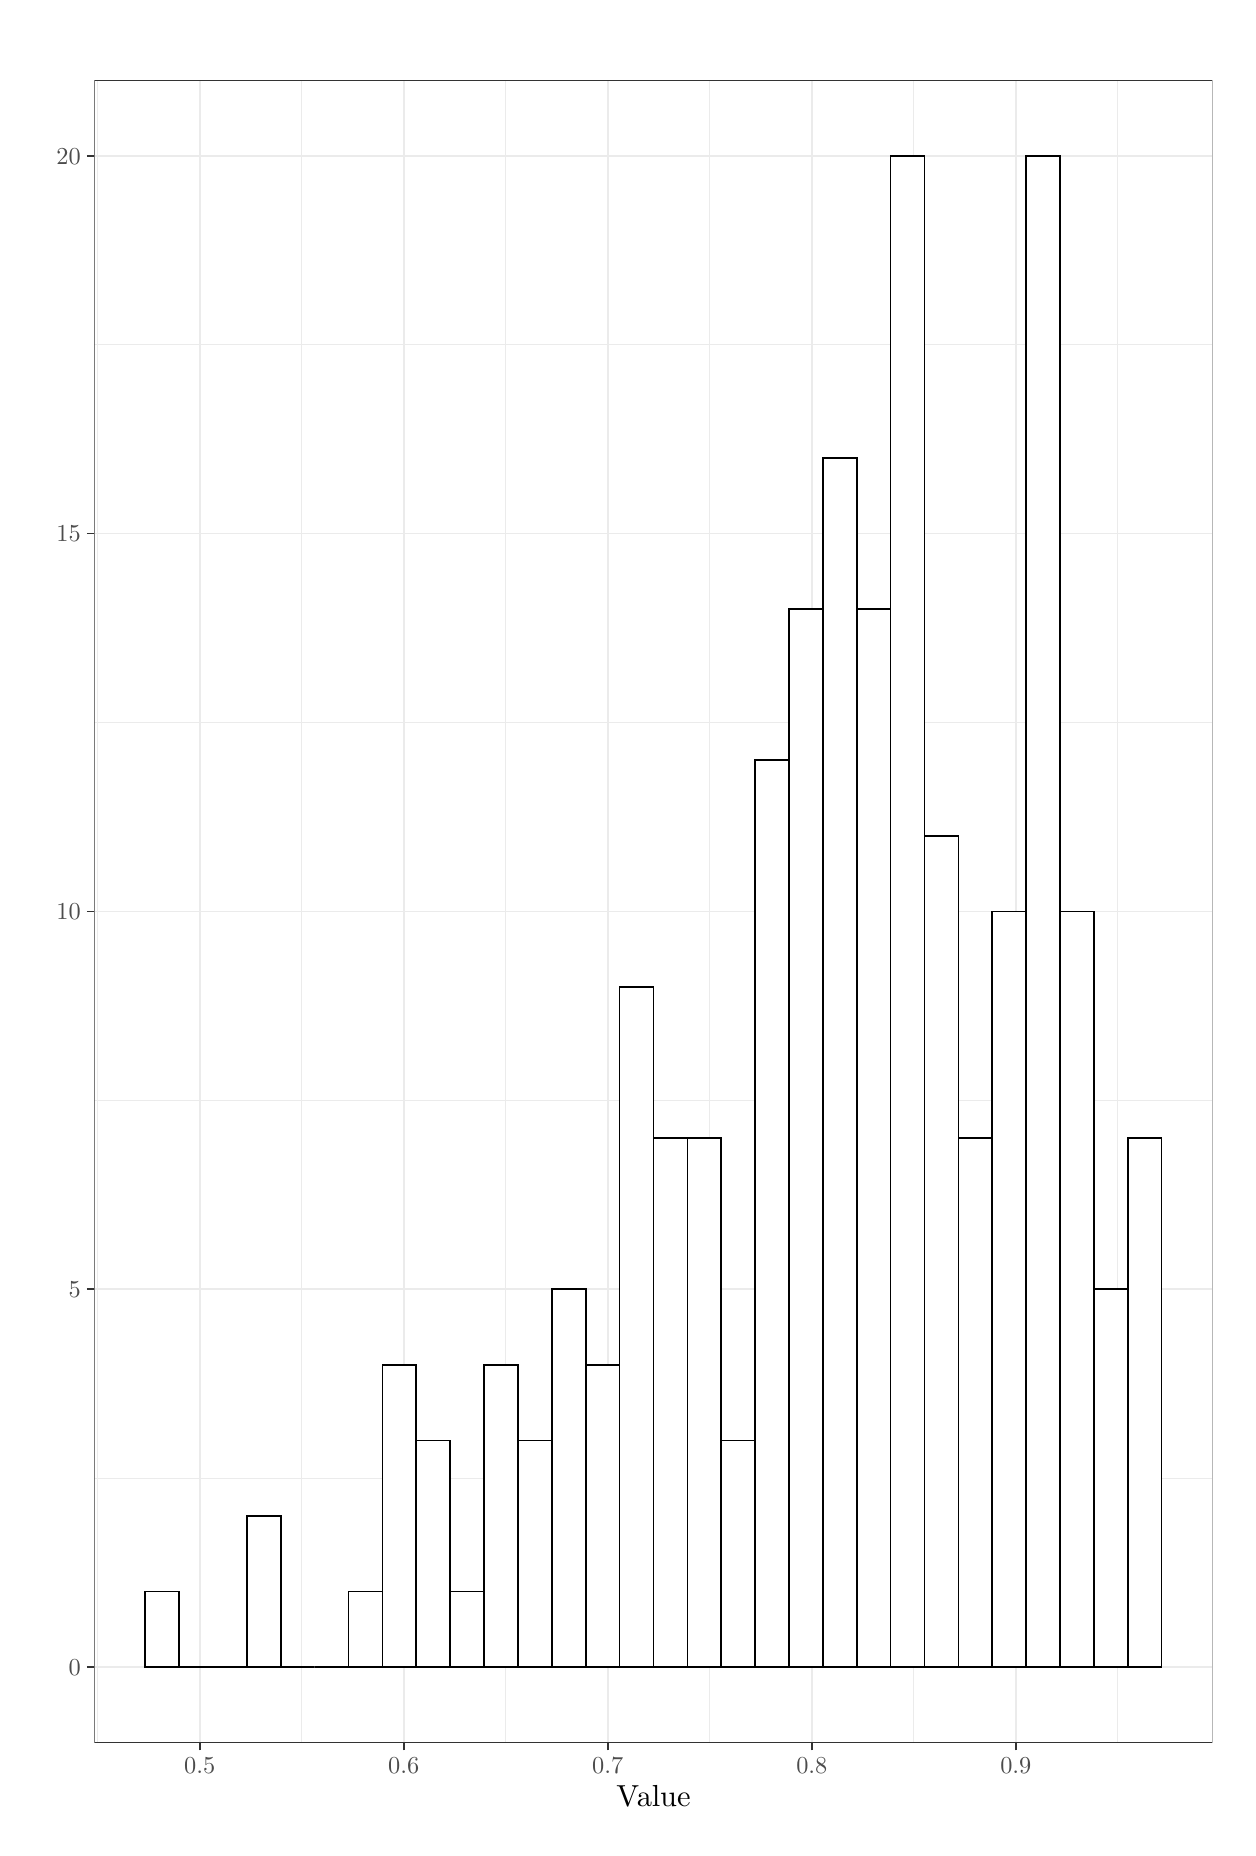
\begin{tikzpicture}[x=1pt,y=1pt]
\definecolor{fillColor}{RGB}{255,255,255}
\path[use as bounding box,fill=fillColor,fill opacity=0.00] (0,0) rectangle (433.62,650.43);
\begin{scope}
\path[clip] (  0.00,  0.00) rectangle (433.62,650.43);
\definecolor{drawColor}{RGB}{255,255,255}
\definecolor{fillColor}{RGB}{255,255,255}

\path[draw=drawColor,line width= 0.6pt,line join=round,line cap=round,fill=fillColor] (  0.00,  0.00) rectangle (433.62,650.43);
\end{scope}
\begin{scope}
\path[clip] ( 24.14, 30.69) rectangle (428.12,631.48);
\definecolor{fillColor}{RGB}{255,255,255}

\path[fill=fillColor] ( 24.14, 30.69) rectangle (428.12,631.48);
\definecolor{drawColor}{gray}{0.92}

\path[draw=drawColor,line width= 0.3pt,line join=round] ( 24.14,126.27) --
	(428.12,126.27);

\path[draw=drawColor,line width= 0.3pt,line join=round] ( 24.14,262.81) --
	(428.12,262.81);

\path[draw=drawColor,line width= 0.3pt,line join=round] ( 24.14,399.36) --
	(428.12,399.36);

\path[draw=drawColor,line width= 0.3pt,line join=round] ( 24.14,535.90) --
	(428.12,535.90);

\path[draw=drawColor,line width= 0.3pt,line join=round] ( 25.34, 30.69) --
	( 25.34,631.48);

\path[draw=drawColor,line width= 0.3pt,line join=round] ( 99.05, 30.69) --
	( 99.05,631.48);

\path[draw=drawColor,line width= 0.3pt,line join=round] (172.77, 30.69) --
	(172.77,631.48);

\path[draw=drawColor,line width= 0.3pt,line join=round] (246.49, 30.69) --
	(246.49,631.48);

\path[draw=drawColor,line width= 0.3pt,line join=round] (320.21, 30.69) --
	(320.21,631.48);

\path[draw=drawColor,line width= 0.3pt,line join=round] (393.93, 30.69) --
	(393.93,631.48);

\path[draw=drawColor,line width= 0.6pt,line join=round] ( 24.14, 57.99) --
	(428.12, 57.99);

\path[draw=drawColor,line width= 0.6pt,line join=round] ( 24.14,194.54) --
	(428.12,194.54);

\path[draw=drawColor,line width= 0.6pt,line join=round] ( 24.14,331.08) --
	(428.12,331.08);

\path[draw=drawColor,line width= 0.6pt,line join=round] ( 24.14,467.63) --
	(428.12,467.63);

\path[draw=drawColor,line width= 0.6pt,line join=round] ( 24.14,604.17) --
	(428.12,604.17);

\path[draw=drawColor,line width= 0.6pt,line join=round] ( 62.19, 30.69) --
	( 62.19,631.48);

\path[draw=drawColor,line width= 0.6pt,line join=round] (135.91, 30.69) --
	(135.91,631.48);

\path[draw=drawColor,line width= 0.6pt,line join=round] (209.63, 30.69) --
	(209.63,631.48);

\path[draw=drawColor,line width= 0.6pt,line join=round] (283.35, 30.69) --
	(283.35,631.48);

\path[draw=drawColor,line width= 0.6pt,line join=round] (357.07, 30.69) --
	(357.07,631.48);
\definecolor{drawColor}{RGB}{0,0,0}

\path[draw=drawColor,line width= 0.6pt,fill=fillColor] ( 42.50, 57.99) rectangle ( 54.74, 85.30);

\path[draw=drawColor,line width= 0.6pt,fill=fillColor] ( 54.74, 57.99) rectangle ( 66.98, 57.99);

\path[draw=drawColor,line width= 0.6pt,fill=fillColor] ( 66.98, 57.99) rectangle ( 79.22, 57.99);

\path[draw=drawColor,line width= 0.6pt,fill=fillColor] ( 79.22, 57.99) rectangle ( 91.47,112.61);

\path[draw=drawColor,line width= 0.6pt,fill=fillColor] ( 91.47, 57.99) rectangle (103.71, 57.99);

\path[draw=drawColor,line width= 0.6pt,fill=fillColor] (103.71, 57.99) rectangle (115.95, 57.99);

\path[draw=drawColor,line width= 0.6pt,fill=fillColor] (115.95, 57.99) rectangle (128.19, 85.30);

\path[draw=drawColor,line width= 0.6pt,fill=fillColor] (128.19, 57.99) rectangle (140.43,167.23);

\path[draw=drawColor,line width= 0.6pt,fill=fillColor] (140.43, 57.99) rectangle (152.68,139.92);

\path[draw=drawColor,line width= 0.6pt,fill=fillColor] (152.68, 57.99) rectangle (164.92, 85.30);

\path[draw=drawColor,line width= 0.6pt,fill=fillColor] (164.92, 57.99) rectangle (177.16,167.23);

\path[draw=drawColor,line width= 0.6pt,fill=fillColor] (177.16, 57.99) rectangle (189.40,139.92);

\path[draw=drawColor,line width= 0.6pt,fill=fillColor] (189.40, 57.99) rectangle (201.64,194.54);

\path[draw=drawColor,line width= 0.6pt,fill=fillColor] (201.64, 57.99) rectangle (213.89,167.23);

\path[draw=drawColor,line width= 0.6pt,fill=fillColor] (213.89, 57.99) rectangle (226.13,303.77);

\path[draw=drawColor,line width= 0.6pt,fill=fillColor] (226.13, 57.99) rectangle (238.37,249.16);

\path[draw=drawColor,line width= 0.6pt,fill=fillColor] (238.37, 57.99) rectangle (250.61,249.16);

\path[draw=drawColor,line width= 0.6pt,fill=fillColor] (250.61, 57.99) rectangle (262.85,139.92);

\path[draw=drawColor,line width= 0.6pt,fill=fillColor] (262.85, 57.99) rectangle (275.10,385.70);

\path[draw=drawColor,line width= 0.6pt,fill=fillColor] (275.10, 57.99) rectangle (287.34,440.32);

\path[draw=drawColor,line width= 0.6pt,fill=fillColor] (287.34, 57.99) rectangle (299.58,494.94);

\path[draw=drawColor,line width= 0.6pt,fill=fillColor] (299.58, 57.99) rectangle (311.82,440.32);

\path[draw=drawColor,line width= 0.6pt,fill=fillColor] (311.82, 57.99) rectangle (324.06,604.17);

\path[draw=drawColor,line width= 0.6pt,fill=fillColor] (324.06, 57.99) rectangle (336.31,358.39);

\path[draw=drawColor,line width= 0.6pt,fill=fillColor] (336.31, 57.99) rectangle (348.55,249.16);

\path[draw=drawColor,line width= 0.6pt,fill=fillColor] (348.55, 57.99) rectangle (360.79,331.08);

\path[draw=drawColor,line width= 0.6pt,fill=fillColor] (360.79, 57.99) rectangle (373.03,604.17);

\path[draw=drawColor,line width= 0.6pt,fill=fillColor] (373.03, 57.99) rectangle (385.27,331.08);

\path[draw=drawColor,line width= 0.6pt,fill=fillColor] (385.27, 57.99) rectangle (397.52,194.54);

\path[draw=drawColor,line width= 0.6pt,fill=fillColor] (397.52, 57.99) rectangle (409.76,249.16);
\definecolor{drawColor}{gray}{0.20}

\path[draw=drawColor,line width= 0.6pt,line join=round,line cap=round] ( 24.14, 30.69) rectangle (428.12,631.48);
\end{scope}
\begin{scope}
\path[clip] (  0.00,  0.00) rectangle (433.62,650.43);
\definecolor{drawColor}{gray}{0.30}

\node[text=drawColor,anchor=base east,inner sep=0pt, outer sep=0pt, scale=  0.88] at ( 19.19, 54.96) {0};

\node[text=drawColor,anchor=base east,inner sep=0pt, outer sep=0pt, scale=  0.88] at ( 19.19,191.51) {5};

\node[text=drawColor,anchor=base east,inner sep=0pt, outer sep=0pt, scale=  0.88] at ( 19.19,328.05) {10};

\node[text=drawColor,anchor=base east,inner sep=0pt, outer sep=0pt, scale=  0.88] at ( 19.19,464.60) {15};

\node[text=drawColor,anchor=base east,inner sep=0pt, outer sep=0pt, scale=  0.88] at ( 19.19,601.14) {20};
\end{scope}
\begin{scope}
\path[clip] (  0.00,  0.00) rectangle (433.62,650.43);
\definecolor{drawColor}{gray}{0.20}

\path[draw=drawColor,line width= 0.6pt,line join=round] ( 21.39, 57.99) --
	( 24.14, 57.99);

\path[draw=drawColor,line width= 0.6pt,line join=round] ( 21.39,194.54) --
	( 24.14,194.54);

\path[draw=drawColor,line width= 0.6pt,line join=round] ( 21.39,331.08) --
	( 24.14,331.08);

\path[draw=drawColor,line width= 0.6pt,line join=round] ( 21.39,467.63) --
	( 24.14,467.63);

\path[draw=drawColor,line width= 0.6pt,line join=round] ( 21.39,604.17) --
	( 24.14,604.17);
\end{scope}
\begin{scope}
\path[clip] (  0.00,  0.00) rectangle (433.62,650.43);
\definecolor{drawColor}{gray}{0.20}

\path[draw=drawColor,line width= 0.6pt,line join=round] ( 62.19, 27.94) --
	( 62.19, 30.69);

\path[draw=drawColor,line width= 0.6pt,line join=round] (135.91, 27.94) --
	(135.91, 30.69);

\path[draw=drawColor,line width= 0.6pt,line join=round] (209.63, 27.94) --
	(209.63, 30.69);

\path[draw=drawColor,line width= 0.6pt,line join=round] (283.35, 27.94) --
	(283.35, 30.69);

\path[draw=drawColor,line width= 0.6pt,line join=round] (357.07, 27.94) --
	(357.07, 30.69);
\end{scope}
\begin{scope}
\path[clip] (  0.00,  0.00) rectangle (433.62,650.43);
\definecolor{drawColor}{gray}{0.30}

\node[text=drawColor,anchor=base,inner sep=0pt, outer sep=0pt, scale=  0.88] at ( 62.19, 19.68) {0.5};

\node[text=drawColor,anchor=base,inner sep=0pt, outer sep=0pt, scale=  0.88] at (135.91, 19.68) {0.6};

\node[text=drawColor,anchor=base,inner sep=0pt, outer sep=0pt, scale=  0.88] at (209.63, 19.68) {0.7};

\node[text=drawColor,anchor=base,inner sep=0pt, outer sep=0pt, scale=  0.88] at (283.35, 19.68) {0.8};

\node[text=drawColor,anchor=base,inner sep=0pt, outer sep=0pt, scale=  0.88] at (357.07, 19.68) {0.9};
\end{scope}
\begin{scope}
\path[clip] (  0.00,  0.00) rectangle (433.62,650.43);
\definecolor{drawColor}{RGB}{0,0,0}

\node[text=drawColor,anchor=base,inner sep=0pt, outer sep=0pt, scale=  1.10] at (226.13,  7.64) {Value};
\end{scope}
\end{tikzpicture}
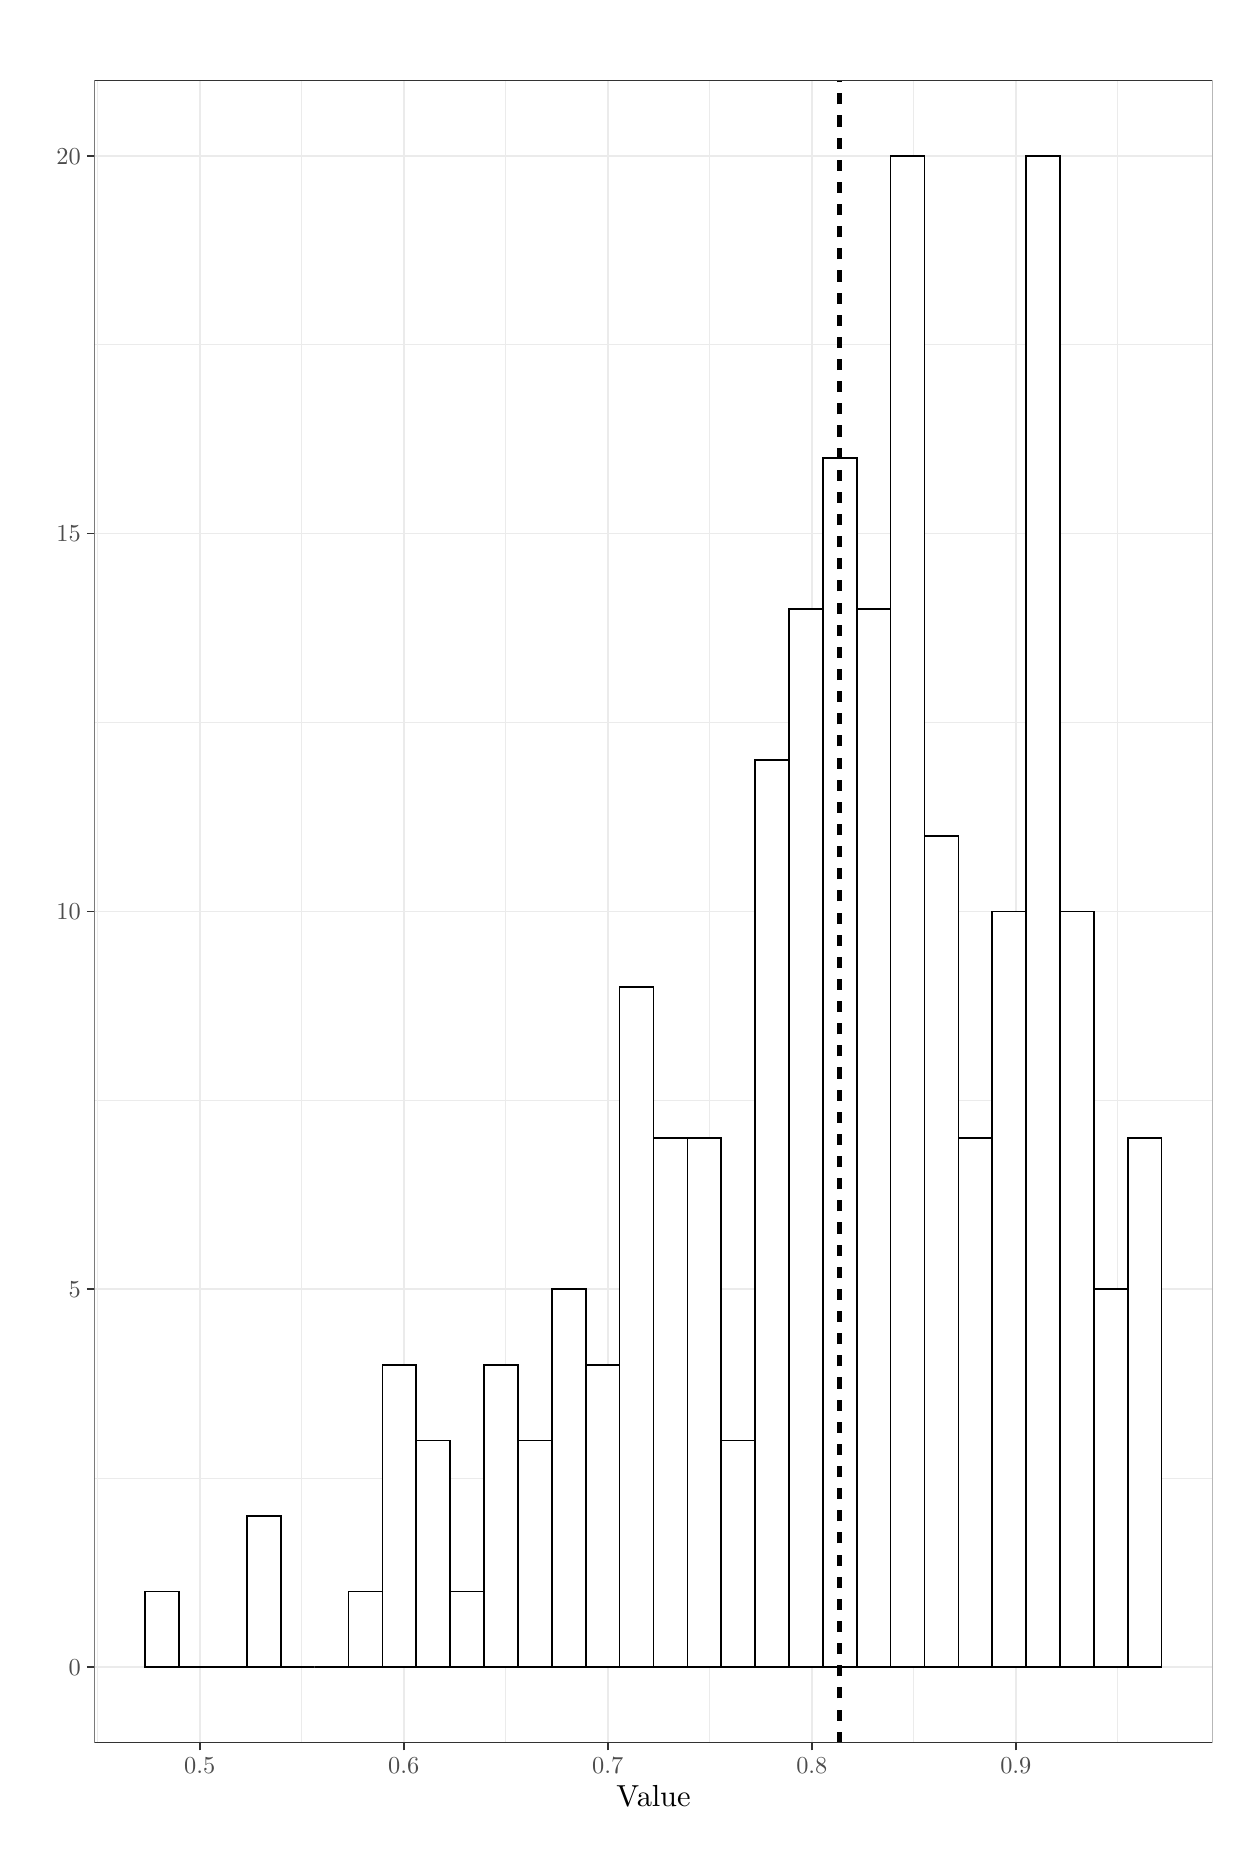
\begin{tikzpicture}[x=1pt,y=1pt]
\definecolor{fillColor}{RGB}{255,255,255}
\path[use as bounding box,fill=fillColor,fill opacity=0.00] (0,0) rectangle (433.62,650.43);
\begin{scope}
\path[clip] (  0.00,  0.00) rectangle (433.62,650.43);
\definecolor{drawColor}{RGB}{255,255,255}
\definecolor{fillColor}{RGB}{255,255,255}

\path[draw=drawColor,line width= 0.6pt,line join=round,line cap=round,fill=fillColor] (  0.00,  0.00) rectangle (433.62,650.43);
\end{scope}
\begin{scope}
\path[clip] ( 24.14, 30.69) rectangle (428.12,631.48);
\definecolor{fillColor}{RGB}{255,255,255}

\path[fill=fillColor] ( 24.14, 30.69) rectangle (428.12,631.48);
\definecolor{drawColor}{gray}{0.92}

\path[draw=drawColor,line width= 0.3pt,line join=round] ( 24.14,126.27) --
	(428.12,126.27);

\path[draw=drawColor,line width= 0.3pt,line join=round] ( 24.14,262.81) --
	(428.12,262.81);

\path[draw=drawColor,line width= 0.3pt,line join=round] ( 24.14,399.36) --
	(428.12,399.36);

\path[draw=drawColor,line width= 0.3pt,line join=round] ( 24.14,535.90) --
	(428.12,535.90);

\path[draw=drawColor,line width= 0.3pt,line join=round] ( 25.34, 30.69) --
	( 25.34,631.48);

\path[draw=drawColor,line width= 0.3pt,line join=round] ( 99.05, 30.69) --
	( 99.05,631.48);

\path[draw=drawColor,line width= 0.3pt,line join=round] (172.77, 30.69) --
	(172.77,631.48);

\path[draw=drawColor,line width= 0.3pt,line join=round] (246.49, 30.69) --
	(246.49,631.48);

\path[draw=drawColor,line width= 0.3pt,line join=round] (320.21, 30.69) --
	(320.21,631.48);

\path[draw=drawColor,line width= 0.3pt,line join=round] (393.93, 30.69) --
	(393.93,631.48);

\path[draw=drawColor,line width= 0.6pt,line join=round] ( 24.14, 57.99) --
	(428.12, 57.99);

\path[draw=drawColor,line width= 0.6pt,line join=round] ( 24.14,194.54) --
	(428.12,194.54);

\path[draw=drawColor,line width= 0.6pt,line join=round] ( 24.14,331.08) --
	(428.12,331.08);

\path[draw=drawColor,line width= 0.6pt,line join=round] ( 24.14,467.63) --
	(428.12,467.63);

\path[draw=drawColor,line width= 0.6pt,line join=round] ( 24.14,604.17) --
	(428.12,604.17);

\path[draw=drawColor,line width= 0.6pt,line join=round] ( 62.19, 30.69) --
	( 62.19,631.48);

\path[draw=drawColor,line width= 0.6pt,line join=round] (135.91, 30.69) --
	(135.91,631.48);

\path[draw=drawColor,line width= 0.6pt,line join=round] (209.63, 30.69) --
	(209.63,631.48);

\path[draw=drawColor,line width= 0.6pt,line join=round] (283.35, 30.69) --
	(283.35,631.48);

\path[draw=drawColor,line width= 0.6pt,line join=round] (357.07, 30.69) --
	(357.07,631.48);
\definecolor{drawColor}{RGB}{0,0,0}

\path[draw=drawColor,line width= 0.6pt,fill=fillColor] ( 42.50, 57.99) rectangle ( 54.74, 85.30);

\path[draw=drawColor,line width= 0.6pt,fill=fillColor] ( 54.74, 57.99) rectangle ( 66.98, 57.99);

\path[draw=drawColor,line width= 0.6pt,fill=fillColor] ( 66.98, 57.99) rectangle ( 79.22, 57.99);

\path[draw=drawColor,line width= 0.6pt,fill=fillColor] ( 79.22, 57.99) rectangle ( 91.47,112.61);

\path[draw=drawColor,line width= 0.6pt,fill=fillColor] ( 91.47, 57.99) rectangle (103.71, 57.99);

\path[draw=drawColor,line width= 0.6pt,fill=fillColor] (103.71, 57.99) rectangle (115.95, 57.99);

\path[draw=drawColor,line width= 0.6pt,fill=fillColor] (115.95, 57.99) rectangle (128.19, 85.30);

\path[draw=drawColor,line width= 0.6pt,fill=fillColor] (128.19, 57.99) rectangle (140.43,167.23);

\path[draw=drawColor,line width= 0.6pt,fill=fillColor] (140.43, 57.99) rectangle (152.68,139.92);

\path[draw=drawColor,line width= 0.6pt,fill=fillColor] (152.68, 57.99) rectangle (164.92, 85.30);

\path[draw=drawColor,line width= 0.6pt,fill=fillColor] (164.92, 57.99) rectangle (177.16,167.23);

\path[draw=drawColor,line width= 0.6pt,fill=fillColor] (177.16, 57.99) rectangle (189.40,139.92);

\path[draw=drawColor,line width= 0.6pt,fill=fillColor] (189.40, 57.99) rectangle (201.64,194.54);

\path[draw=drawColor,line width= 0.6pt,fill=fillColor] (201.64, 57.99) rectangle (213.89,167.23);

\path[draw=drawColor,line width= 0.6pt,fill=fillColor] (213.89, 57.99) rectangle (226.13,303.77);

\path[draw=drawColor,line width= 0.6pt,fill=fillColor] (226.13, 57.99) rectangle (238.37,249.16);

\path[draw=drawColor,line width= 0.6pt,fill=fillColor] (238.37, 57.99) rectangle (250.61,249.16);

\path[draw=drawColor,line width= 0.6pt,fill=fillColor] (250.61, 57.99) rectangle (262.85,139.92);

\path[draw=drawColor,line width= 0.6pt,fill=fillColor] (262.85, 57.99) rectangle (275.10,385.70);

\path[draw=drawColor,line width= 0.6pt,fill=fillColor] (275.10, 57.99) rectangle (287.34,440.32);

\path[draw=drawColor,line width= 0.6pt,fill=fillColor] (287.34, 57.99) rectangle (299.58,494.94);

\path[draw=drawColor,line width= 0.6pt,fill=fillColor] (299.58, 57.99) rectangle (311.82,440.32);

\path[draw=drawColor,line width= 0.6pt,fill=fillColor] (311.82, 57.99) rectangle (324.06,604.17);

\path[draw=drawColor,line width= 0.6pt,fill=fillColor] (324.06, 57.99) rectangle (336.31,358.39);

\path[draw=drawColor,line width= 0.6pt,fill=fillColor] (336.31, 57.99) rectangle (348.55,249.16);

\path[draw=drawColor,line width= 0.6pt,fill=fillColor] (348.55, 57.99) rectangle (360.79,331.08);

\path[draw=drawColor,line width= 0.6pt,fill=fillColor] (360.79, 57.99) rectangle (373.03,604.17);

\path[draw=drawColor,line width= 0.6pt,fill=fillColor] (373.03, 57.99) rectangle (385.27,331.08);

\path[draw=drawColor,line width= 0.6pt,fill=fillColor] (385.27, 57.99) rectangle (397.52,194.54);

\path[draw=drawColor,line width= 0.6pt,fill=fillColor] (397.52, 57.99) rectangle (409.76,249.16);

\path[draw=drawColor,line width= 1.7pt,dash pattern=on 4pt off 4pt ,line join=round] (293.33, 30.69) -- (293.33,631.48);
\definecolor{drawColor}{gray}{0.20}

\path[draw=drawColor,line width= 0.6pt,line join=round,line cap=round] ( 24.14, 30.69) rectangle (428.12,631.48);
\end{scope}
\begin{scope}
\path[clip] (  0.00,  0.00) rectangle (433.62,650.43);
\definecolor{drawColor}{gray}{0.30}

\node[text=drawColor,anchor=base east,inner sep=0pt, outer sep=0pt, scale=  0.88] at ( 19.19, 54.96) {0};

\node[text=drawColor,anchor=base east,inner sep=0pt, outer sep=0pt, scale=  0.88] at ( 19.19,191.51) {5};

\node[text=drawColor,anchor=base east,inner sep=0pt, outer sep=0pt, scale=  0.88] at ( 19.19,328.05) {10};

\node[text=drawColor,anchor=base east,inner sep=0pt, outer sep=0pt, scale=  0.88] at ( 19.19,464.60) {15};

\node[text=drawColor,anchor=base east,inner sep=0pt, outer sep=0pt, scale=  0.88] at ( 19.19,601.14) {20};
\end{scope}
\begin{scope}
\path[clip] (  0.00,  0.00) rectangle (433.62,650.43);
\definecolor{drawColor}{gray}{0.20}

\path[draw=drawColor,line width= 0.6pt,line join=round] ( 21.39, 57.99) --
	( 24.14, 57.99);

\path[draw=drawColor,line width= 0.6pt,line join=round] ( 21.39,194.54) --
	( 24.14,194.54);

\path[draw=drawColor,line width= 0.6pt,line join=round] ( 21.39,331.08) --
	( 24.14,331.08);

\path[draw=drawColor,line width= 0.6pt,line join=round] ( 21.39,467.63) --
	( 24.14,467.63);

\path[draw=drawColor,line width= 0.6pt,line join=round] ( 21.39,604.17) --
	( 24.14,604.17);
\end{scope}
\begin{scope}
\path[clip] (  0.00,  0.00) rectangle (433.62,650.43);
\definecolor{drawColor}{gray}{0.20}

\path[draw=drawColor,line width= 0.6pt,line join=round] ( 62.19, 27.94) --
	( 62.19, 30.69);

\path[draw=drawColor,line width= 0.6pt,line join=round] (135.91, 27.94) --
	(135.91, 30.69);

\path[draw=drawColor,line width= 0.6pt,line join=round] (209.63, 27.94) --
	(209.63, 30.69);

\path[draw=drawColor,line width= 0.6pt,line join=round] (283.35, 27.94) --
	(283.35, 30.69);

\path[draw=drawColor,line width= 0.6pt,line join=round] (357.07, 27.94) --
	(357.07, 30.69);
\end{scope}
\begin{scope}
\path[clip] (  0.00,  0.00) rectangle (433.62,650.43);
\definecolor{drawColor}{gray}{0.30}

\node[text=drawColor,anchor=base,inner sep=0pt, outer sep=0pt, scale=  0.88] at ( 62.19, 19.68) {0.5};

\node[text=drawColor,anchor=base,inner sep=0pt, outer sep=0pt, scale=  0.88] at (135.91, 19.68) {0.6};

\node[text=drawColor,anchor=base,inner sep=0pt, outer sep=0pt, scale=  0.88] at (209.63, 19.68) {0.7};

\node[text=drawColor,anchor=base,inner sep=0pt, outer sep=0pt, scale=  0.88] at (283.35, 19.68) {0.8};

\node[text=drawColor,anchor=base,inner sep=0pt, outer sep=0pt, scale=  0.88] at (357.07, 19.68) {0.9};
\end{scope}
\begin{scope}
\path[clip] (  0.00,  0.00) rectangle (433.62,650.43);
\definecolor{drawColor}{RGB}{0,0,0}

\node[text=drawColor,anchor=base,inner sep=0pt, outer sep=0pt, scale=  1.10] at (226.13,  7.64) {Value};
\end{scope}
\end{tikzpicture}
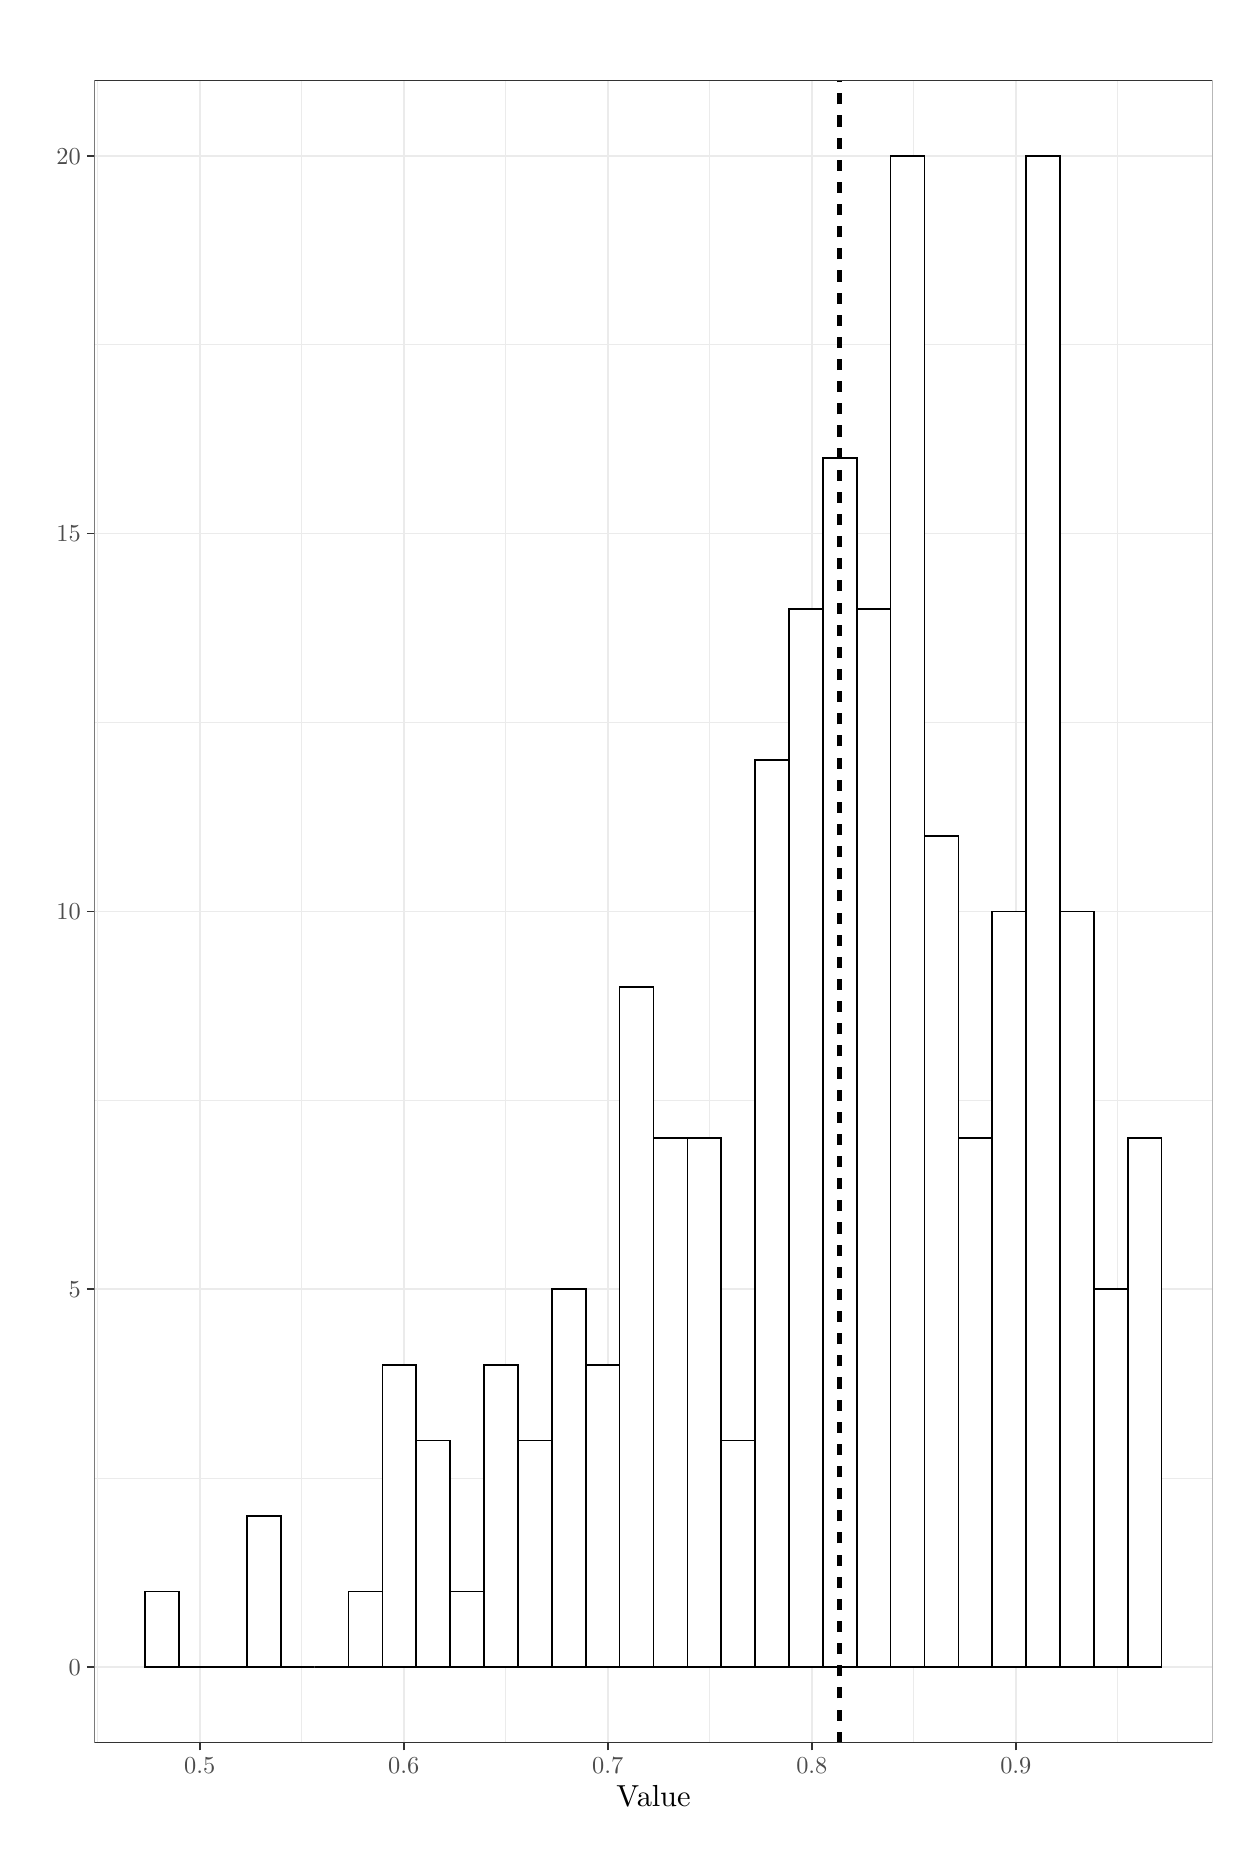
\begin{tikzpicture}[x=1pt,y=1pt]
\definecolor{fillColor}{RGB}{255,255,255}
\path[use as bounding box,fill=fillColor,fill opacity=0.00] (0,0) rectangle (433.62,650.43);
\begin{scope}
\path[clip] (  0.00,  0.00) rectangle (433.62,650.43);
\definecolor{drawColor}{RGB}{255,255,255}
\definecolor{fillColor}{RGB}{255,255,255}

\path[draw=drawColor,line width= 0.6pt,line join=round,line cap=round,fill=fillColor] (  0.00,  0.00) rectangle (433.62,650.43);
\end{scope}
\begin{scope}
\path[clip] ( 24.14, 30.69) rectangle (428.12,631.48);
\definecolor{fillColor}{RGB}{255,255,255}

\path[fill=fillColor] ( 24.14, 30.69) rectangle (428.12,631.48);
\definecolor{drawColor}{gray}{0.92}

\path[draw=drawColor,line width= 0.3pt,line join=round] ( 24.14,126.27) --
	(428.12,126.27);

\path[draw=drawColor,line width= 0.3pt,line join=round] ( 24.14,262.81) --
	(428.12,262.81);

\path[draw=drawColor,line width= 0.3pt,line join=round] ( 24.14,399.36) --
	(428.12,399.36);

\path[draw=drawColor,line width= 0.3pt,line join=round] ( 24.14,535.90) --
	(428.12,535.90);

\path[draw=drawColor,line width= 0.3pt,line join=round] ( 25.34, 30.69) --
	( 25.34,631.48);

\path[draw=drawColor,line width= 0.3pt,line join=round] ( 99.05, 30.69) --
	( 99.05,631.48);

\path[draw=drawColor,line width= 0.3pt,line join=round] (172.77, 30.69) --
	(172.77,631.48);

\path[draw=drawColor,line width= 0.3pt,line join=round] (246.49, 30.69) --
	(246.49,631.48);

\path[draw=drawColor,line width= 0.3pt,line join=round] (320.21, 30.69) --
	(320.21,631.48);

\path[draw=drawColor,line width= 0.3pt,line join=round] (393.93, 30.69) --
	(393.93,631.48);

\path[draw=drawColor,line width= 0.6pt,line join=round] ( 24.14, 57.99) --
	(428.12, 57.99);

\path[draw=drawColor,line width= 0.6pt,line join=round] ( 24.14,194.54) --
	(428.12,194.54);

\path[draw=drawColor,line width= 0.6pt,line join=round] ( 24.14,331.08) --
	(428.12,331.08);

\path[draw=drawColor,line width= 0.6pt,line join=round] ( 24.14,467.63) --
	(428.12,467.63);

\path[draw=drawColor,line width= 0.6pt,line join=round] ( 24.14,604.17) --
	(428.12,604.17);

\path[draw=drawColor,line width= 0.6pt,line join=round] ( 62.19, 30.69) --
	( 62.19,631.48);

\path[draw=drawColor,line width= 0.6pt,line join=round] (135.91, 30.69) --
	(135.91,631.48);

\path[draw=drawColor,line width= 0.6pt,line join=round] (209.63, 30.69) --
	(209.63,631.48);

\path[draw=drawColor,line width= 0.6pt,line join=round] (283.35, 30.69) --
	(283.35,631.48);

\path[draw=drawColor,line width= 0.6pt,line join=round] (357.07, 30.69) --
	(357.07,631.48);
\definecolor{drawColor}{RGB}{0,0,0}

\path[draw=drawColor,line width= 0.6pt,fill=fillColor] ( 42.50, 57.99) rectangle ( 54.74, 85.30);

\path[draw=drawColor,line width= 0.6pt,fill=fillColor] ( 54.74, 57.99) rectangle ( 66.98, 57.99);

\path[draw=drawColor,line width= 0.6pt,fill=fillColor] ( 66.98, 57.99) rectangle ( 79.22, 57.99);

\path[draw=drawColor,line width= 0.6pt,fill=fillColor] ( 79.22, 57.99) rectangle ( 91.47,112.61);

\path[draw=drawColor,line width= 0.6pt,fill=fillColor] ( 91.47, 57.99) rectangle (103.71, 57.99);

\path[draw=drawColor,line width= 0.6pt,fill=fillColor] (103.71, 57.99) rectangle (115.95, 57.99);

\path[draw=drawColor,line width= 0.6pt,fill=fillColor] (115.95, 57.99) rectangle (128.19, 85.30);

\path[draw=drawColor,line width= 0.6pt,fill=fillColor] (128.19, 57.99) rectangle (140.43,167.23);

\path[draw=drawColor,line width= 0.6pt,fill=fillColor] (140.43, 57.99) rectangle (152.68,139.92);

\path[draw=drawColor,line width= 0.6pt,fill=fillColor] (152.68, 57.99) rectangle (164.92, 85.30);

\path[draw=drawColor,line width= 0.6pt,fill=fillColor] (164.92, 57.99) rectangle (177.16,167.23);

\path[draw=drawColor,line width= 0.6pt,fill=fillColor] (177.16, 57.99) rectangle (189.40,139.92);

\path[draw=drawColor,line width= 0.6pt,fill=fillColor] (189.40, 57.99) rectangle (201.64,194.54);

\path[draw=drawColor,line width= 0.6pt,fill=fillColor] (201.64, 57.99) rectangle (213.89,167.23);

\path[draw=drawColor,line width= 0.6pt,fill=fillColor] (213.89, 57.99) rectangle (226.13,303.77);

\path[draw=drawColor,line width= 0.6pt,fill=fillColor] (226.13, 57.99) rectangle (238.37,249.16);

\path[draw=drawColor,line width= 0.6pt,fill=fillColor] (238.37, 57.99) rectangle (250.61,249.16);

\path[draw=drawColor,line width= 0.6pt,fill=fillColor] (250.61, 57.99) rectangle (262.85,139.92);

\path[draw=drawColor,line width= 0.6pt,fill=fillColor] (262.85, 57.99) rectangle (275.10,385.70);

\path[draw=drawColor,line width= 0.6pt,fill=fillColor] (275.10, 57.99) rectangle (287.34,440.32);

\path[draw=drawColor,line width= 0.6pt,fill=fillColor] (287.34, 57.99) rectangle (299.58,494.94);

\path[draw=drawColor,line width= 0.6pt,fill=fillColor] (299.58, 57.99) rectangle (311.82,440.32);

\path[draw=drawColor,line width= 0.6pt,fill=fillColor] (311.82, 57.99) rectangle (324.06,604.17);

\path[draw=drawColor,line width= 0.6pt,fill=fillColor] (324.06, 57.99) rectangle (336.31,358.39);

\path[draw=drawColor,line width= 0.6pt,fill=fillColor] (336.31, 57.99) rectangle (348.55,249.16);

\path[draw=drawColor,line width= 0.6pt,fill=fillColor] (348.55, 57.99) rectangle (360.79,331.08);

\path[draw=drawColor,line width= 0.6pt,fill=fillColor] (360.79, 57.99) rectangle (373.03,604.17);

\path[draw=drawColor,line width= 0.6pt,fill=fillColor] (373.03, 57.99) rectangle (385.27,331.08);

\path[draw=drawColor,line width= 0.6pt,fill=fillColor] (385.27, 57.99) rectangle (397.52,194.54);

\path[draw=drawColor,line width= 0.6pt,fill=fillColor] (397.52, 57.99) rectangle (409.76,249.16);

\path[draw=drawColor,line width= 1.7pt,dash pattern=on 4pt off 4pt ,line join=round] (293.33, 30.69) -- (293.33,631.48);
\definecolor{drawColor}{gray}{0.20}

\path[draw=drawColor,line width= 0.6pt,line join=round,line cap=round] ( 24.14, 30.69) rectangle (428.12,631.48);
\end{scope}
\begin{scope}
\path[clip] (  0.00,  0.00) rectangle (433.62,650.43);
\definecolor{drawColor}{gray}{0.30}

\node[text=drawColor,anchor=base east,inner sep=0pt, outer sep=0pt, scale=  0.88] at ( 19.19, 54.96) {0};

\node[text=drawColor,anchor=base east,inner sep=0pt, outer sep=0pt, scale=  0.88] at ( 19.19,191.51) {5};

\node[text=drawColor,anchor=base east,inner sep=0pt, outer sep=0pt, scale=  0.88] at ( 19.19,328.05) {10};

\node[text=drawColor,anchor=base east,inner sep=0pt, outer sep=0pt, scale=  0.88] at ( 19.19,464.60) {15};

\node[text=drawColor,anchor=base east,inner sep=0pt, outer sep=0pt, scale=  0.88] at ( 19.19,601.14) {20};
\end{scope}
\begin{scope}
\path[clip] (  0.00,  0.00) rectangle (433.62,650.43);
\definecolor{drawColor}{gray}{0.20}

\path[draw=drawColor,line width= 0.6pt,line join=round] ( 21.39, 57.99) --
	( 24.14, 57.99);

\path[draw=drawColor,line width= 0.6pt,line join=round] ( 21.39,194.54) --
	( 24.14,194.54);

\path[draw=drawColor,line width= 0.6pt,line join=round] ( 21.39,331.08) --
	( 24.14,331.08);

\path[draw=drawColor,line width= 0.6pt,line join=round] ( 21.39,467.63) --
	( 24.14,467.63);

\path[draw=drawColor,line width= 0.6pt,line join=round] ( 21.39,604.17) --
	( 24.14,604.17);
\end{scope}
\begin{scope}
\path[clip] (  0.00,  0.00) rectangle (433.62,650.43);
\definecolor{drawColor}{gray}{0.20}

\path[draw=drawColor,line width= 0.6pt,line join=round] ( 62.19, 27.94) --
	( 62.19, 30.69);

\path[draw=drawColor,line width= 0.6pt,line join=round] (135.91, 27.94) --
	(135.91, 30.69);

\path[draw=drawColor,line width= 0.6pt,line join=round] (209.63, 27.94) --
	(209.63, 30.69);

\path[draw=drawColor,line width= 0.6pt,line join=round] (283.35, 27.94) --
	(283.35, 30.69);

\path[draw=drawColor,line width= 0.6pt,line join=round] (357.07, 27.94) --
	(357.07, 30.69);
\end{scope}
\begin{scope}
\path[clip] (  0.00,  0.00) rectangle (433.62,650.43);
\definecolor{drawColor}{gray}{0.30}

\node[text=drawColor,anchor=base,inner sep=0pt, outer sep=0pt, scale=  0.88] at ( 62.19, 19.68) {0.5};

\node[text=drawColor,anchor=base,inner sep=0pt, outer sep=0pt, scale=  0.88] at (135.91, 19.68) {0.6};

\node[text=drawColor,anchor=base,inner sep=0pt, outer sep=0pt, scale=  0.88] at (209.63, 19.68) {0.7};

\node[text=drawColor,anchor=base,inner sep=0pt, outer sep=0pt, scale=  0.88] at (283.35, 19.68) {0.8};

\node[text=drawColor,anchor=base,inner sep=0pt, outer sep=0pt, scale=  0.88] at (357.07, 19.68) {0.9};
\end{scope}
\begin{scope}
\path[clip] (  0.00,  0.00) rectangle (433.62,650.43);
\definecolor{drawColor}{RGB}{0,0,0}

\node[text=drawColor,anchor=base,inner sep=0pt, outer sep=0pt, scale=  1.10] at (226.13,  7.64) {Value};
\end{scope}
\end{tikzpicture}
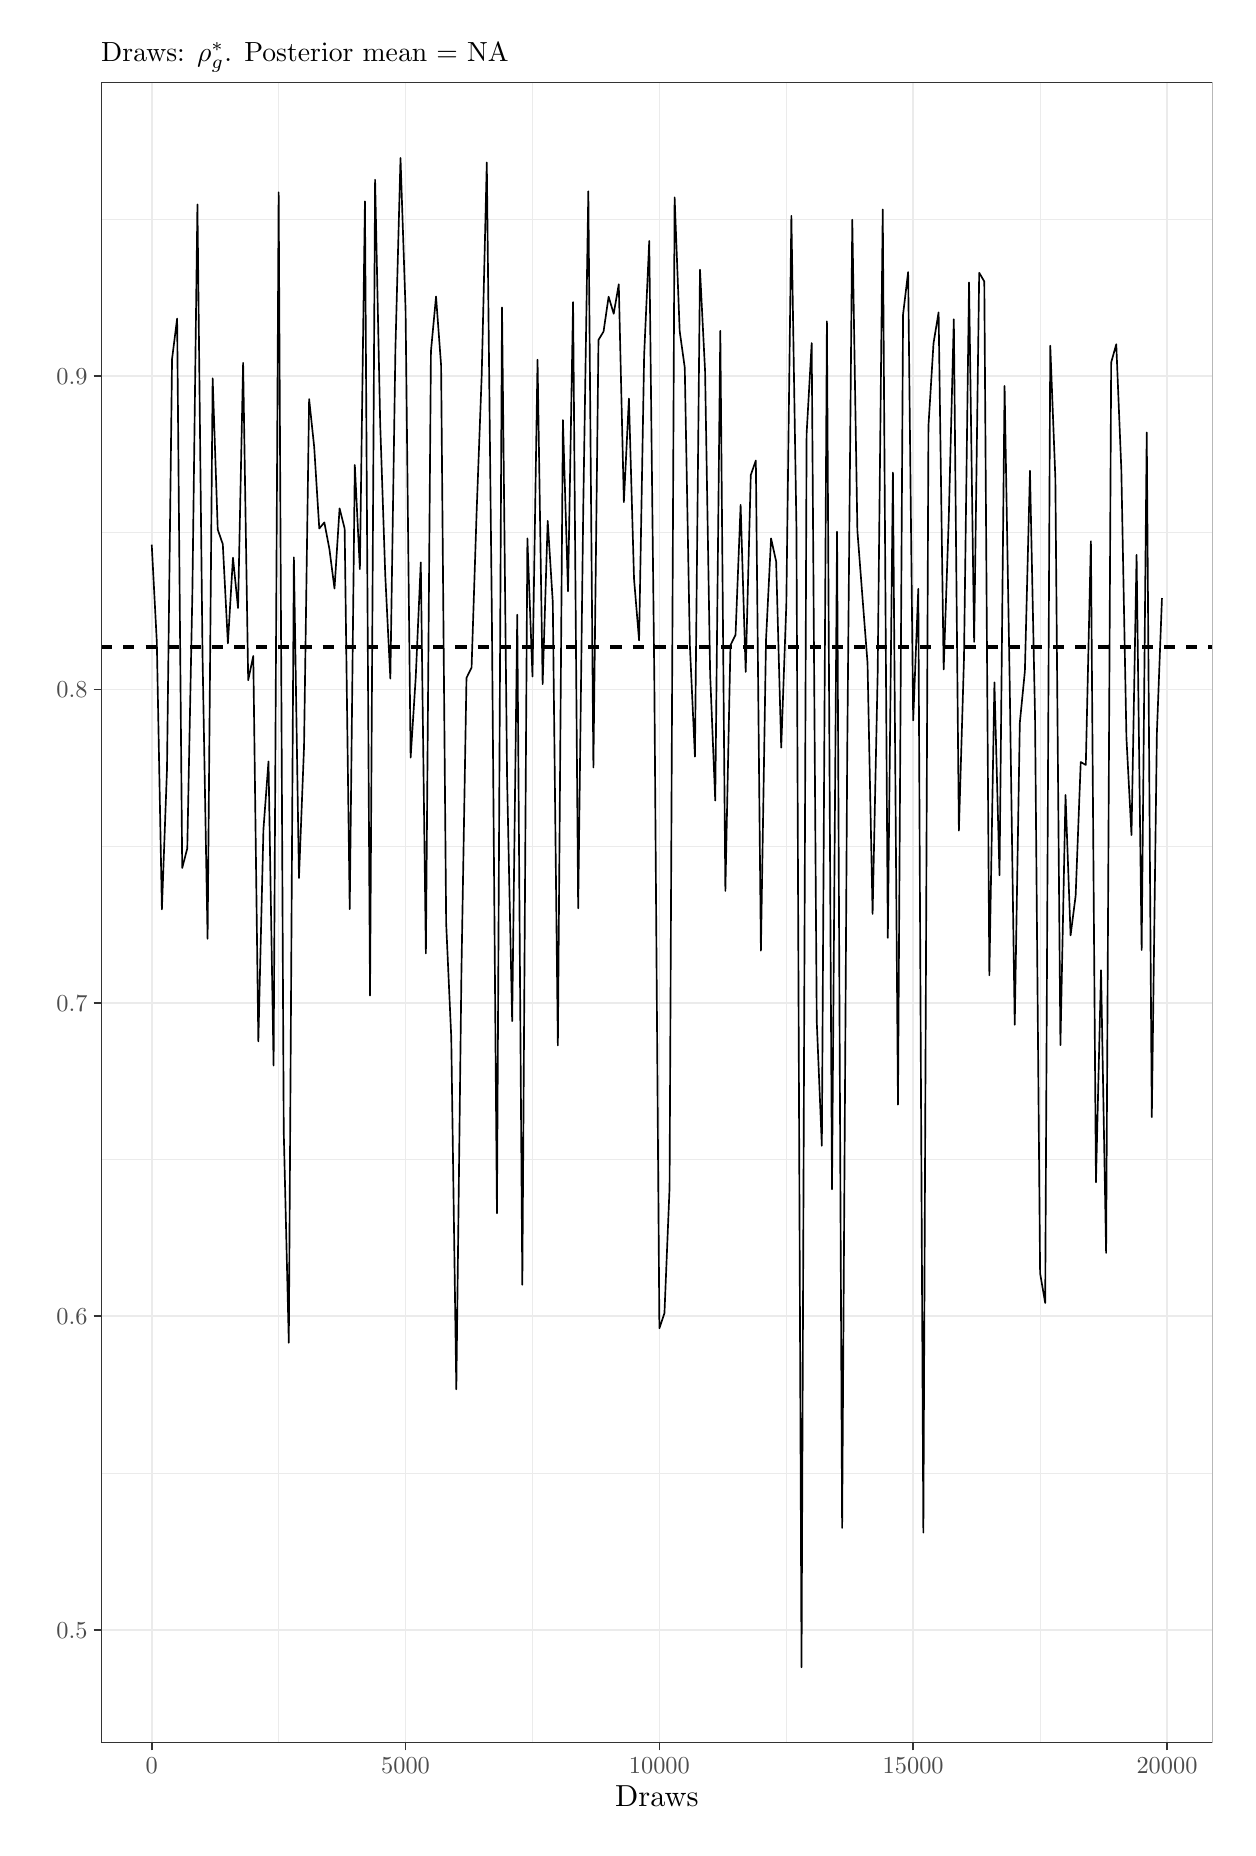
\begin{tikzpicture}[x=1pt,y=1pt]
\definecolor{fillColor}{RGB}{255,255,255}
\path[use as bounding box,fill=fillColor,fill opacity=0.00] (0,0) rectangle (433.62,650.43);
\begin{scope}
\path[clip] (  0.00,  0.00) rectangle (433.62,650.43);
\definecolor{drawColor}{RGB}{255,255,255}
\definecolor{fillColor}{RGB}{255,255,255}

\path[draw=drawColor,line width= 0.6pt,line join=round,line cap=round,fill=fillColor] (  0.00,  0.00) rectangle (433.62,650.43);
\end{scope}
\begin{scope}
\path[clip] ( 26.58, 30.69) rectangle (428.12,630.60);
\definecolor{fillColor}{RGB}{255,255,255}

\path[fill=fillColor] ( 26.58, 30.69) rectangle (428.12,630.60);
\definecolor{drawColor}{gray}{0.92}

\path[draw=drawColor,line width= 0.3pt,line join=round] ( 26.58,128.16) --
	(428.12,128.16);

\path[draw=drawColor,line width= 0.3pt,line join=round] ( 26.58,241.41) --
	(428.12,241.41);

\path[draw=drawColor,line width= 0.3pt,line join=round] ( 26.58,354.65) --
	(428.12,354.65);

\path[draw=drawColor,line width= 0.3pt,line join=round] ( 26.58,467.90) --
	(428.12,467.90);

\path[draw=drawColor,line width= 0.3pt,line join=round] ( 26.58,581.15) --
	(428.12,581.15);

\path[draw=drawColor,line width= 0.3pt,line join=round] ( 90.69, 30.69) --
	( 90.69,630.60);

\path[draw=drawColor,line width= 0.3pt,line join=round] (182.41, 30.69) --
	(182.41,630.60);

\path[draw=drawColor,line width= 0.3pt,line join=round] (274.13, 30.69) --
	(274.13,630.60);

\path[draw=drawColor,line width= 0.3pt,line join=round] (365.84, 30.69) --
	(365.84,630.60);

\path[draw=drawColor,line width= 0.6pt,line join=round] ( 26.58, 71.54) --
	(428.12, 71.54);

\path[draw=drawColor,line width= 0.6pt,line join=round] ( 26.58,184.79) --
	(428.12,184.79);

\path[draw=drawColor,line width= 0.6pt,line join=round] ( 26.58,298.03) --
	(428.12,298.03);

\path[draw=drawColor,line width= 0.6pt,line join=round] ( 26.58,411.28) --
	(428.12,411.28);

\path[draw=drawColor,line width= 0.6pt,line join=round] ( 26.58,524.52) --
	(428.12,524.52);

\path[draw=drawColor,line width= 0.6pt,line join=round] ( 44.83, 30.69) --
	( 44.83,630.60);

\path[draw=drawColor,line width= 0.6pt,line join=round] (136.55, 30.69) --
	(136.55,630.60);

\path[draw=drawColor,line width= 0.6pt,line join=round] (228.27, 30.69) --
	(228.27,630.60);

\path[draw=drawColor,line width= 0.6pt,line join=round] (319.98, 30.69) --
	(319.98,630.60);

\path[draw=drawColor,line width= 0.6pt,line join=round] (411.70, 30.69) --
	(411.70,630.60);
\definecolor{drawColor}{RGB}{0,0,0}

\path[draw=drawColor,line width= 0.6pt,line join=round] ( 44.83,463.59) --
	( 46.67,428.37) --
	( 48.50,331.84) --
	( 50.34,382.39) --
	( 52.17,530.69) --
	( 54.00,545.31) --
	( 55.84,346.78) --
	( 57.67,353.85) --
	( 59.51,446.02) --
	( 61.34,586.54) --
	( 63.18,423.93) --
	( 65.01,321.20) --
	( 66.84,523.73) --
	( 68.68,469.08) --
	( 70.51,463.77) --
	( 72.35,427.96) --
	( 74.18,458.88) --
	( 76.02,440.71) --
	( 77.85,529.30) --
	( 79.68,414.62) --
	( 81.52,423.39) --
	( 83.35,284.11) --
	( 85.19,360.72) --
	( 87.02,385.30) --
	( 88.86,275.40) --
	( 90.69,590.93) --
	( 92.53,251.55) --
	( 94.36,175.19) --
	( 96.19,459.07) --
	( 98.03,343.15) --
	( 99.86,390.52) --
	(101.70,516.22) --
	(103.53,498.94) --
	(105.37,469.45) --
	(107.20,471.65) --
	(109.03,462.04) --
	(110.87,447.74) --
	(112.70,476.73) --
	(114.54,469.39) --
	(116.37,331.90) --
	(118.21,492.39) --
	(120.04,454.76) --
	(121.87,587.66) --
	(123.71,300.66) --
	(125.54,595.48) --
	(127.38,507.41) --
	(129.21,452.62) --
	(131.05,415.22) --
	(132.88,534.30) --
	(134.72,603.33) --
	(136.55,548.60) --
	(138.38,386.65) --
	(140.22,415.59) --
	(142.05,457.21) --
	(143.89,315.90) --
	(145.72,533.48) --
	(147.56,553.26) --
	(149.39,528.40) --
	(151.22,326.80) --
	(153.06,285.59) --
	(154.89,158.39) --
	(156.73,308.89) --
	(158.56,415.45) --
	(160.40,419.20) --
	(162.23,475.51) --
	(164.06,524.78) --
	(165.90,601.71) --
	(167.73,438.20) --
	(169.57,221.98) --
	(171.40,549.29) --
	(173.24,378.87) --
	(175.07,291.44) --
	(176.91,438.26) --
	(178.74,196.17) --
	(180.57,465.86) --
	(182.41,415.97) --
	(184.24,530.46) --
	(186.08,413.22) --
	(187.91,472.20) --
	(189.75,442.79) --
	(191.58,282.66) --
	(193.41,508.63) --
	(195.25,446.73) --
	(197.08,551.25) --
	(198.92,332.21) --
	(200.75,476.23) --
	(202.59,591.31) --
	(204.42,383.08) --
	(206.26,537.58) --
	(208.09,540.62) --
	(209.92,553.20) --
	(211.76,547.06) --
	(213.59,557.70) --
	(215.43,479.00) --
	(217.26,516.41) --
	(219.10,451.31) --
	(220.93,429.01) --
	(222.76,532.12) --
	(224.60,573.35) --
	(226.43,415.71) --
	(228.27,180.46) --
	(230.10,185.93) --
	(231.94,231.14) --
	(233.77,589.09) --
	(235.60,540.78) --
	(237.44,527.55) --
	(239.27,427.52) --
	(241.11,387.02) --
	(242.94,562.96) --
	(244.78,526.23) --
	(246.61,416.77) --
	(248.45,371.11) --
	(250.28,540.87) --
	(252.11,338.45) --
	(253.95,427.28) --
	(255.78,430.97) --
	(257.62,477.97) --
	(259.45,417.62) --
	(261.29,488.78) --
	(263.12,494.01) --
	(264.95,316.90) --
	(266.79,429.06) --
	(268.62,465.86) --
	(270.46,457.55) --
	(272.29,390.25) --
	(274.13,441.83) --
	(275.96,582.42) --
	(277.79,469.68) --
	(279.63, 57.95) --
	(281.46,503.56) --
	(283.30,536.46) --
	(285.13,291.41) --
	(286.97,246.39) --
	(288.80,544.33) --
	(290.64,230.64) --
	(292.47,468.28) --
	(294.30,108.31) --
	(296.14,388.24) --
	(297.97,581.03) --
	(299.81,468.69) --
	(301.64,444.72) --
	(303.48,420.86) --
	(305.31,330.17) --
	(307.14,416.96) --
	(308.98,584.76) --
	(310.81,321.51) --
	(312.65,489.66) --
	(314.48,261.26) --
	(316.32,546.81) --
	(318.15,562.12) --
	(319.98,400.11) --
	(321.82,447.65) --
	(323.65,106.63) --
	(325.49,506.45) --
	(327.32,536.38) --
	(329.16,547.56) --
	(330.99,418.51) --
	(332.83,472.99) --
	(334.66,545.06) --
	(336.49,360.28) --
	(338.33,422.33) --
	(340.16,558.34) --
	(342.00,428.50) --
	(343.83,561.86) --
	(345.67,558.72) --
	(347.50,308.01) --
	(349.33,413.84) --
	(351.17,344.16) --
	(353.00,520.96) --
	(354.84,414.36) --
	(356.67,290.09) --
	(358.51,399.24) --
	(360.34,417.94) --
	(362.18,490.29) --
	(364.01,401.49) --
	(365.84,200.30) --
	(367.68,189.61) --
	(369.51,535.50) --
	(371.35,487.65) --
	(373.18,282.78) --
	(375.02,373.15) --
	(376.85,322.42) --
	(378.68,336.74) --
	(380.52,385.08) --
	(382.35,383.99) --
	(384.19,464.86) --
	(386.02,233.18) --
	(387.86,309.83) --
	(389.69,207.67) --
	(391.52,529.45) --
	(393.36,536.03) --
	(395.19,490.71) --
	(397.03,393.89) --
	(398.86,358.64) --
	(400.70,459.94) --
	(402.53,317.13) --
	(404.37,504.19) --
	(406.20,256.73) --
	(408.03,395.41) --
	(409.87,444.33);

\path[draw=drawColor,line width= 1.7pt,dash pattern=on 4pt off 4pt ,line join=round] ( 26.58,426.61) -- (428.12,426.61);
\definecolor{drawColor}{gray}{0.20}

\path[draw=drawColor,line width= 0.6pt,line join=round,line cap=round] ( 26.58, 30.69) rectangle (428.12,630.60);
\end{scope}
\begin{scope}
\path[clip] (  0.00,  0.00) rectangle (433.62,650.43);
\definecolor{drawColor}{gray}{0.30}

\node[text=drawColor,anchor=base east,inner sep=0pt, outer sep=0pt, scale=  0.88] at ( 21.63, 68.51) {0.5};

\node[text=drawColor,anchor=base east,inner sep=0pt, outer sep=0pt, scale=  0.88] at ( 21.63,181.76) {0.6};

\node[text=drawColor,anchor=base east,inner sep=0pt, outer sep=0pt, scale=  0.88] at ( 21.63,295.00) {0.7};

\node[text=drawColor,anchor=base east,inner sep=0pt, outer sep=0pt, scale=  0.88] at ( 21.63,408.25) {0.8};

\node[text=drawColor,anchor=base east,inner sep=0pt, outer sep=0pt, scale=  0.88] at ( 21.63,521.49) {0.9};
\end{scope}
\begin{scope}
\path[clip] (  0.00,  0.00) rectangle (433.62,650.43);
\definecolor{drawColor}{gray}{0.20}

\path[draw=drawColor,line width= 0.6pt,line join=round] ( 23.83, 71.54) --
	( 26.58, 71.54);

\path[draw=drawColor,line width= 0.6pt,line join=round] ( 23.83,184.79) --
	( 26.58,184.79);

\path[draw=drawColor,line width= 0.6pt,line join=round] ( 23.83,298.03) --
	( 26.58,298.03);

\path[draw=drawColor,line width= 0.6pt,line join=round] ( 23.83,411.28) --
	( 26.58,411.28);

\path[draw=drawColor,line width= 0.6pt,line join=round] ( 23.83,524.52) --
	( 26.58,524.52);
\end{scope}
\begin{scope}
\path[clip] (  0.00,  0.00) rectangle (433.62,650.43);
\definecolor{drawColor}{gray}{0.20}

\path[draw=drawColor,line width= 0.6pt,line join=round] ( 44.83, 27.94) --
	( 44.83, 30.69);

\path[draw=drawColor,line width= 0.6pt,line join=round] (136.55, 27.94) --
	(136.55, 30.69);

\path[draw=drawColor,line width= 0.6pt,line join=round] (228.27, 27.94) --
	(228.27, 30.69);

\path[draw=drawColor,line width= 0.6pt,line join=round] (319.98, 27.94) --
	(319.98, 30.69);

\path[draw=drawColor,line width= 0.6pt,line join=round] (411.70, 27.94) --
	(411.70, 30.69);
\end{scope}
\begin{scope}
\path[clip] (  0.00,  0.00) rectangle (433.62,650.43);
\definecolor{drawColor}{gray}{0.30}

\node[text=drawColor,anchor=base,inner sep=0pt, outer sep=0pt, scale=  0.88] at ( 44.83, 19.68) {0};

\node[text=drawColor,anchor=base,inner sep=0pt, outer sep=0pt, scale=  0.88] at (136.55, 19.68) {5000};

\node[text=drawColor,anchor=base,inner sep=0pt, outer sep=0pt, scale=  0.88] at (228.27, 19.68) {10000};

\node[text=drawColor,anchor=base,inner sep=0pt, outer sep=0pt, scale=  0.88] at (319.98, 19.68) {15000};

\node[text=drawColor,anchor=base,inner sep=0pt, outer sep=0pt, scale=  0.88] at (411.70, 19.68) {20000};
\end{scope}
\begin{scope}
\path[clip] (  0.00,  0.00) rectangle (433.62,650.43);
\definecolor{drawColor}{RGB}{0,0,0}

\node[text=drawColor,anchor=base,inner sep=0pt, outer sep=0pt, scale=  1.10] at (227.35,  7.64) {Draws};
\end{scope}
\begin{scope}
\path[clip] (  0.00,  0.00) rectangle (433.62,650.43);
\definecolor{drawColor}{RGB}{0,0,0}

\node[text=drawColor,anchor=base west,inner sep=0pt, outer sep=0pt, scale=  1.00] at ( 26.58,638.04) {Draws: $\rho_g^*$. Posterior mean = NA};
\end{scope}
\end{tikzpicture}
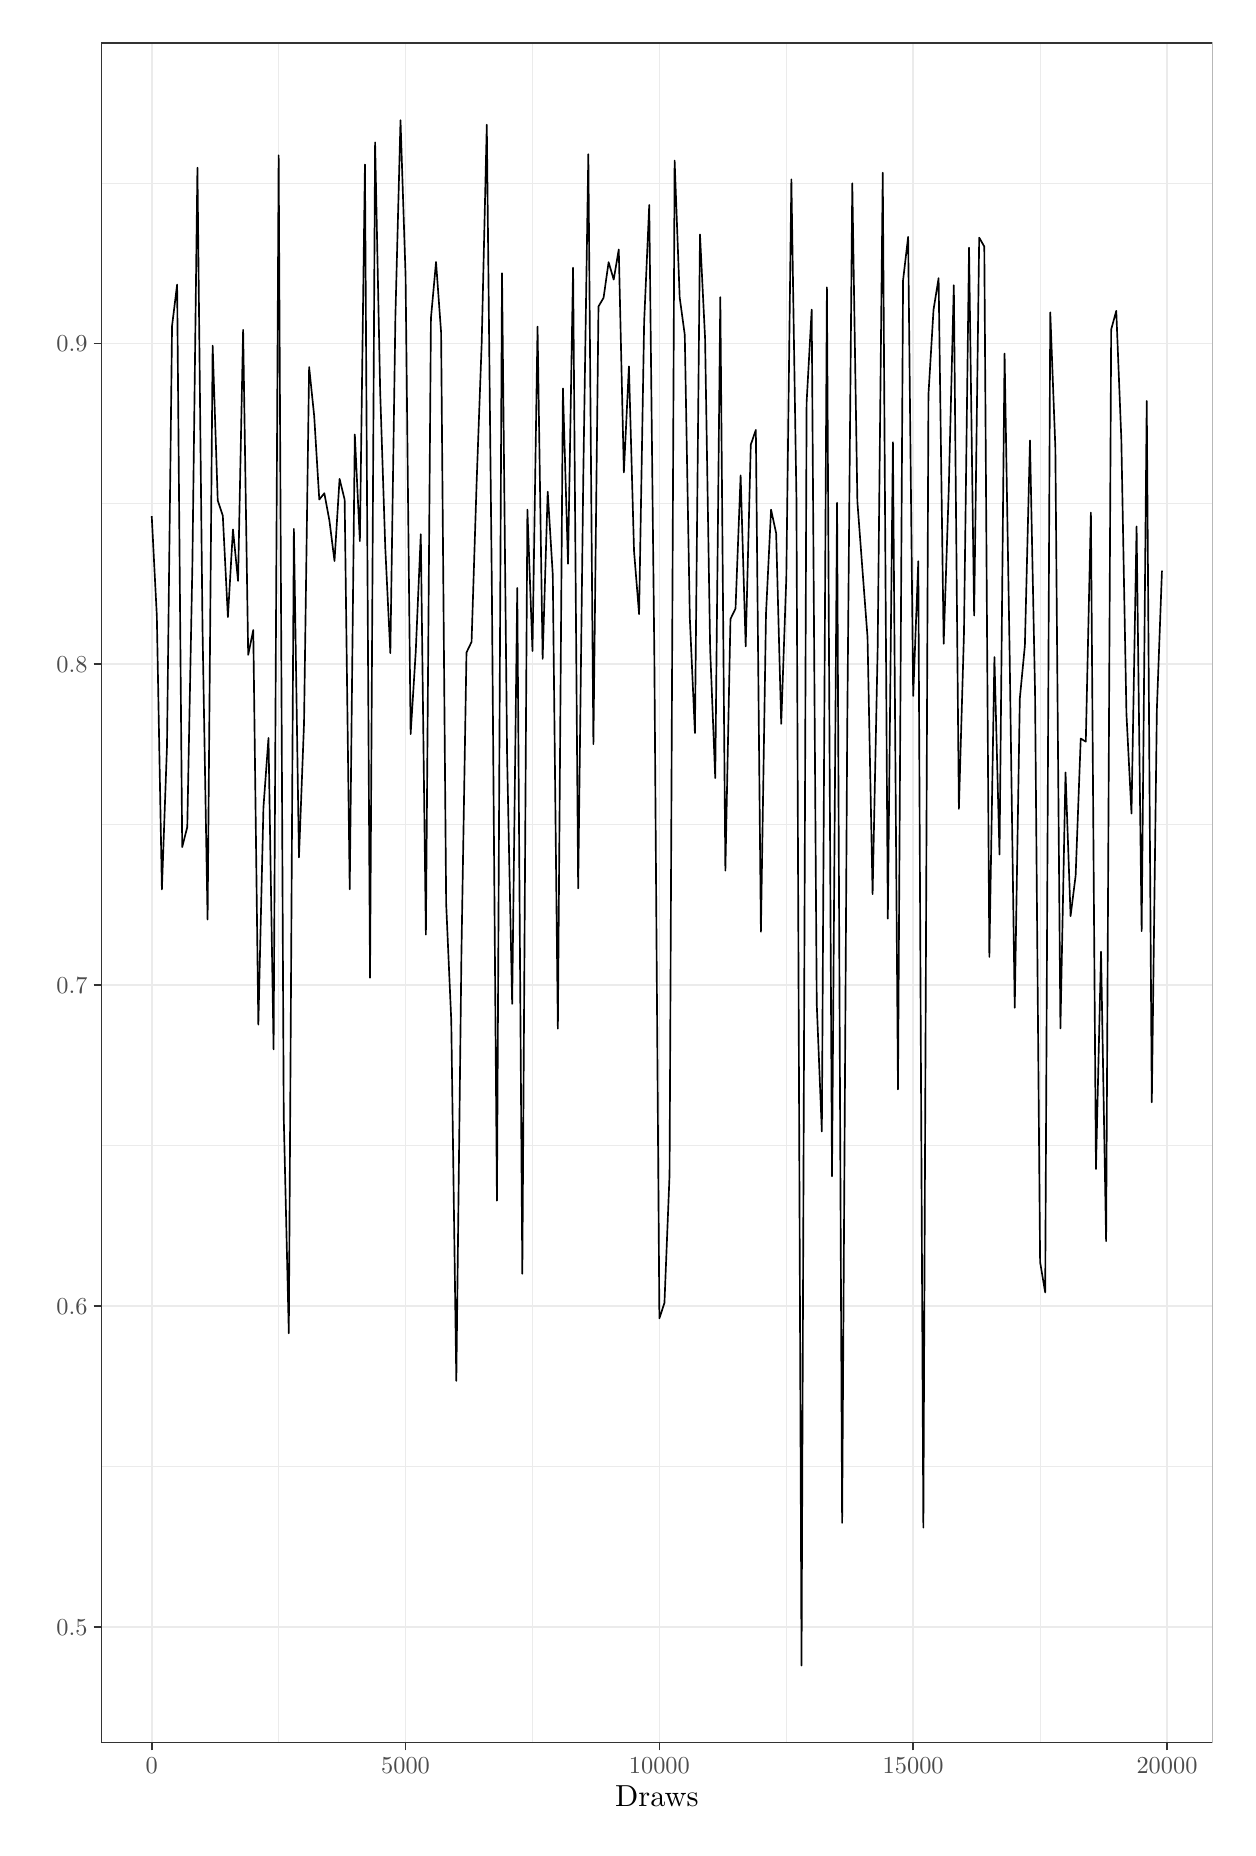
\begin{tikzpicture}[x=1pt,y=1pt]
\definecolor{fillColor}{RGB}{255,255,255}
\path[use as bounding box,fill=fillColor,fill opacity=0.00] (0,0) rectangle (433.62,650.43);
\begin{scope}
\path[clip] (  0.00,  0.00) rectangle (433.62,650.43);
\definecolor{drawColor}{RGB}{255,255,255}
\definecolor{fillColor}{RGB}{255,255,255}

\path[draw=drawColor,line width= 0.6pt,line join=round,line cap=round,fill=fillColor] (  0.00,  0.00) rectangle (433.62,650.43);
\end{scope}
\begin{scope}
\path[clip] ( 26.58, 30.69) rectangle (428.12,644.93);
\definecolor{fillColor}{RGB}{255,255,255}

\path[fill=fillColor] ( 26.58, 30.69) rectangle (428.12,644.93);
\definecolor{drawColor}{gray}{0.92}

\path[draw=drawColor,line width= 0.3pt,line join=round] ( 26.58,130.49) --
	(428.12,130.49);

\path[draw=drawColor,line width= 0.3pt,line join=round] ( 26.58,246.44) --
	(428.12,246.44);

\path[draw=drawColor,line width= 0.3pt,line join=round] ( 26.58,362.39) --
	(428.12,362.39);

\path[draw=drawColor,line width= 0.3pt,line join=round] ( 26.58,478.35) --
	(428.12,478.35);

\path[draw=drawColor,line width= 0.3pt,line join=round] ( 26.58,594.30) --
	(428.12,594.30);

\path[draw=drawColor,line width= 0.3pt,line join=round] ( 90.69, 30.69) --
	( 90.69,644.93);

\path[draw=drawColor,line width= 0.3pt,line join=round] (182.41, 30.69) --
	(182.41,644.93);

\path[draw=drawColor,line width= 0.3pt,line join=round] (274.13, 30.69) --
	(274.13,644.93);

\path[draw=drawColor,line width= 0.3pt,line join=round] (365.84, 30.69) --
	(365.84,644.93);

\path[draw=drawColor,line width= 0.6pt,line join=round] ( 26.58, 72.52) --
	(428.12, 72.52);

\path[draw=drawColor,line width= 0.6pt,line join=round] ( 26.58,188.47) --
	(428.12,188.47);

\path[draw=drawColor,line width= 0.6pt,line join=round] ( 26.58,304.42) --
	(428.12,304.42);

\path[draw=drawColor,line width= 0.6pt,line join=round] ( 26.58,420.37) --
	(428.12,420.37);

\path[draw=drawColor,line width= 0.6pt,line join=round] ( 26.58,536.32) --
	(428.12,536.32);

\path[draw=drawColor,line width= 0.6pt,line join=round] ( 44.83, 30.69) --
	( 44.83,644.93);

\path[draw=drawColor,line width= 0.6pt,line join=round] (136.55, 30.69) --
	(136.55,644.93);

\path[draw=drawColor,line width= 0.6pt,line join=round] (228.27, 30.69) --
	(228.27,644.93);

\path[draw=drawColor,line width= 0.6pt,line join=round] (319.98, 30.69) --
	(319.98,644.93);

\path[draw=drawColor,line width= 0.6pt,line join=round] (411.70, 30.69) --
	(411.70,644.93);
\definecolor{drawColor}{RGB}{0,0,0}

\path[draw=drawColor,line width= 0.6pt,line join=round] ( 44.83,473.93) --
	( 46.67,437.87) --
	( 48.50,339.03) --
	( 50.34,390.79) --
	( 52.17,542.64) --
	( 54.00,557.60) --
	( 55.84,354.33) --
	( 57.67,361.57) --
	( 59.51,455.94) --
	( 61.34,599.82) --
	( 63.18,433.32) --
	( 65.01,328.14) --
	( 66.84,535.51) --
	( 68.68,479.56) --
	( 70.51,474.12) --
	( 72.35,437.45) --
	( 74.18,469.11) --
	( 76.02,450.51) --
	( 77.85,541.22) --
	( 79.68,423.79) --
	( 81.52,432.77) --
	( 83.35,290.17) --
	( 85.19,368.61) --
	( 87.02,393.78) --
	( 88.86,281.24) --
	( 90.69,604.32) --
	( 92.53,256.83) --
	( 94.36,178.65) --
	( 96.19,469.30) --
	( 98.03,350.61) --
	( 99.86,399.11) --
	(101.70,527.81) --
	(103.53,510.13) --
	(105.37,479.93) --
	(107.20,482.18) --
	(109.03,472.35) --
	(110.87,457.70) --
	(112.70,487.38) --
	(114.54,479.87) --
	(116.37,339.10) --
	(118.21,503.42) --
	(120.04,464.89) --
	(121.87,600.97) --
	(123.71,307.11) --
	(125.54,608.97) --
	(127.38,518.80) --
	(129.21,462.70) --
	(131.05,424.41) --
	(132.88,546.33) --
	(134.72,617.01) --
	(136.55,560.97) --
	(138.38,395.16) --
	(140.22,424.78) --
	(142.05,467.40) --
	(143.89,322.71) --
	(145.72,545.49) --
	(147.56,565.75) --
	(149.39,540.29) --
	(151.22,333.87) --
	(153.06,291.68) --
	(154.89,161.44) --
	(156.73,315.53) --
	(158.56,424.64) --
	(160.40,428.48) --
	(162.23,486.14) --
	(164.06,536.58) --
	(165.90,615.35) --
	(167.73,447.94) --
	(169.57,226.55) --
	(171.40,561.68) --
	(173.24,387.19) --
	(175.07,297.67) --
	(176.91,448.00) --
	(178.74,200.13) --
	(180.57,476.26) --
	(182.41,425.18) --
	(184.24,542.40) --
	(186.08,422.36) --
	(187.91,482.75) --
	(189.75,452.64) --
	(191.58,288.68) --
	(193.41,520.05) --
	(195.25,456.67) --
	(197.08,563.68) --
	(198.92,339.42) --
	(200.75,486.87) --
	(202.59,604.71) --
	(204.42,391.49) --
	(206.26,549.69) --
	(208.09,552.80) --
	(209.92,565.68) --
	(211.76,559.40) --
	(213.59,570.29) --
	(215.43,489.71) --
	(217.26,528.02) --
	(219.10,461.36) --
	(220.93,438.53) --
	(222.76,544.10) --
	(224.60,586.32) --
	(226.43,424.91) --
	(228.27,184.04) --
	(230.10,189.64) --
	(231.94,235.93) --
	(233.77,602.43) --
	(235.60,552.96) --
	(237.44,539.42) --
	(239.27,437.00) --
	(241.11,395.53) --
	(242.94,575.68) --
	(244.78,538.06) --
	(246.61,425.99) --
	(248.45,379.24) --
	(250.28,553.05) --
	(252.11,345.81) --
	(253.95,436.75) --
	(255.78,440.53) --
	(257.62,488.66) --
	(259.45,426.86) --
	(261.29,499.72) --
	(263.12,505.08) --
	(264.95,323.73) --
	(266.79,438.58) --
	(268.62,476.26) --
	(270.46,467.74) --
	(272.29,398.84) --
	(274.13,451.66) --
	(275.96,595.60) --
	(277.79,480.17) --
	(279.63, 58.61) --
	(281.46,514.85) --
	(283.30,548.55) --
	(285.13,297.64) --
	(286.97,251.55) --
	(288.80,556.60) --
	(290.64,235.41) --
	(292.47,478.74) --
	(294.30,110.16) --
	(296.14,396.78) --
	(297.97,594.18) --
	(299.81,479.15) --
	(301.64,454.61) --
	(303.48,430.18) --
	(305.31,337.32) --
	(307.14,426.19) --
	(308.98,598.00) --
	(310.81,328.46) --
	(312.65,500.62) --
	(314.48,266.77) --
	(316.32,559.14) --
	(318.15,574.81) --
	(319.98,408.94) --
	(321.82,457.61) --
	(323.65,108.44) --
	(325.49,517.81) --
	(327.32,548.46) --
	(329.16,559.91) --
	(330.99,427.78) --
	(332.83,483.55) --
	(334.66,557.35) --
	(336.49,368.16) --
	(338.33,431.68) --
	(340.16,570.94) --
	(342.00,438.00) --
	(343.83,574.55) --
	(345.67,571.34) --
	(347.50,314.63) --
	(349.33,422.99) --
	(351.17,351.65) --
	(353.00,532.68) --
	(354.84,423.53) --
	(356.67,296.28) --
	(358.51,408.04) --
	(360.34,427.19) --
	(362.18,501.27) --
	(364.01,410.35) --
	(365.84,204.35) --
	(367.68,193.41) --
	(369.51,547.56) --
	(371.35,498.56) --
	(373.18,288.80) --
	(375.02,381.33) --
	(376.85,329.39) --
	(378.68,344.05) --
	(380.52,393.55) --
	(382.35,392.43) --
	(384.19,475.23) --
	(386.02,238.01) --
	(387.86,316.50) --
	(389.69,211.90) --
	(391.52,541.36) --
	(393.36,548.10) --
	(395.19,501.70) --
	(397.03,402.57) --
	(398.86,366.48) --
	(400.70,470.20) --
	(402.53,323.97) --
	(404.37,515.50) --
	(406.20,262.13) --
	(408.03,404.12) --
	(409.87,454.21);
\definecolor{drawColor}{gray}{0.20}

\path[draw=drawColor,line width= 0.6pt,line join=round,line cap=round] ( 26.58, 30.69) rectangle (428.12,644.93);
\end{scope}
\begin{scope}
\path[clip] (  0.00,  0.00) rectangle (433.62,650.43);
\definecolor{drawColor}{gray}{0.30}

\node[text=drawColor,anchor=base east,inner sep=0pt, outer sep=0pt, scale=  0.88] at ( 21.63, 69.49) {0.5};

\node[text=drawColor,anchor=base east,inner sep=0pt, outer sep=0pt, scale=  0.88] at ( 21.63,185.44) {0.6};

\node[text=drawColor,anchor=base east,inner sep=0pt, outer sep=0pt, scale=  0.88] at ( 21.63,301.39) {0.7};

\node[text=drawColor,anchor=base east,inner sep=0pt, outer sep=0pt, scale=  0.88] at ( 21.63,417.34) {0.8};

\node[text=drawColor,anchor=base east,inner sep=0pt, outer sep=0pt, scale=  0.88] at ( 21.63,533.29) {0.9};
\end{scope}
\begin{scope}
\path[clip] (  0.00,  0.00) rectangle (433.62,650.43);
\definecolor{drawColor}{gray}{0.20}

\path[draw=drawColor,line width= 0.6pt,line join=round] ( 23.83, 72.52) --
	( 26.58, 72.52);

\path[draw=drawColor,line width= 0.6pt,line join=round] ( 23.83,188.47) --
	( 26.58,188.47);

\path[draw=drawColor,line width= 0.6pt,line join=round] ( 23.83,304.42) --
	( 26.58,304.42);

\path[draw=drawColor,line width= 0.6pt,line join=round] ( 23.83,420.37) --
	( 26.58,420.37);

\path[draw=drawColor,line width= 0.6pt,line join=round] ( 23.83,536.32) --
	( 26.58,536.32);
\end{scope}
\begin{scope}
\path[clip] (  0.00,  0.00) rectangle (433.62,650.43);
\definecolor{drawColor}{gray}{0.20}

\path[draw=drawColor,line width= 0.6pt,line join=round] ( 44.83, 27.94) --
	( 44.83, 30.69);

\path[draw=drawColor,line width= 0.6pt,line join=round] (136.55, 27.94) --
	(136.55, 30.69);

\path[draw=drawColor,line width= 0.6pt,line join=round] (228.27, 27.94) --
	(228.27, 30.69);

\path[draw=drawColor,line width= 0.6pt,line join=round] (319.98, 27.94) --
	(319.98, 30.69);

\path[draw=drawColor,line width= 0.6pt,line join=round] (411.70, 27.94) --
	(411.70, 30.69);
\end{scope}
\begin{scope}
\path[clip] (  0.00,  0.00) rectangle (433.62,650.43);
\definecolor{drawColor}{gray}{0.30}

\node[text=drawColor,anchor=base,inner sep=0pt, outer sep=0pt, scale=  0.88] at ( 44.83, 19.68) {0};

\node[text=drawColor,anchor=base,inner sep=0pt, outer sep=0pt, scale=  0.88] at (136.55, 19.68) {5000};

\node[text=drawColor,anchor=base,inner sep=0pt, outer sep=0pt, scale=  0.88] at (228.27, 19.68) {10000};

\node[text=drawColor,anchor=base,inner sep=0pt, outer sep=0pt, scale=  0.88] at (319.98, 19.68) {15000};

\node[text=drawColor,anchor=base,inner sep=0pt, outer sep=0pt, scale=  0.88] at (411.70, 19.68) {20000};
\end{scope}
\begin{scope}
\path[clip] (  0.00,  0.00) rectangle (433.62,650.43);
\definecolor{drawColor}{RGB}{0,0,0}

\node[text=drawColor,anchor=base,inner sep=0pt, outer sep=0pt, scale=  1.10] at (227.35,  7.64) {Draws};
\end{scope}
\end{tikzpicture}
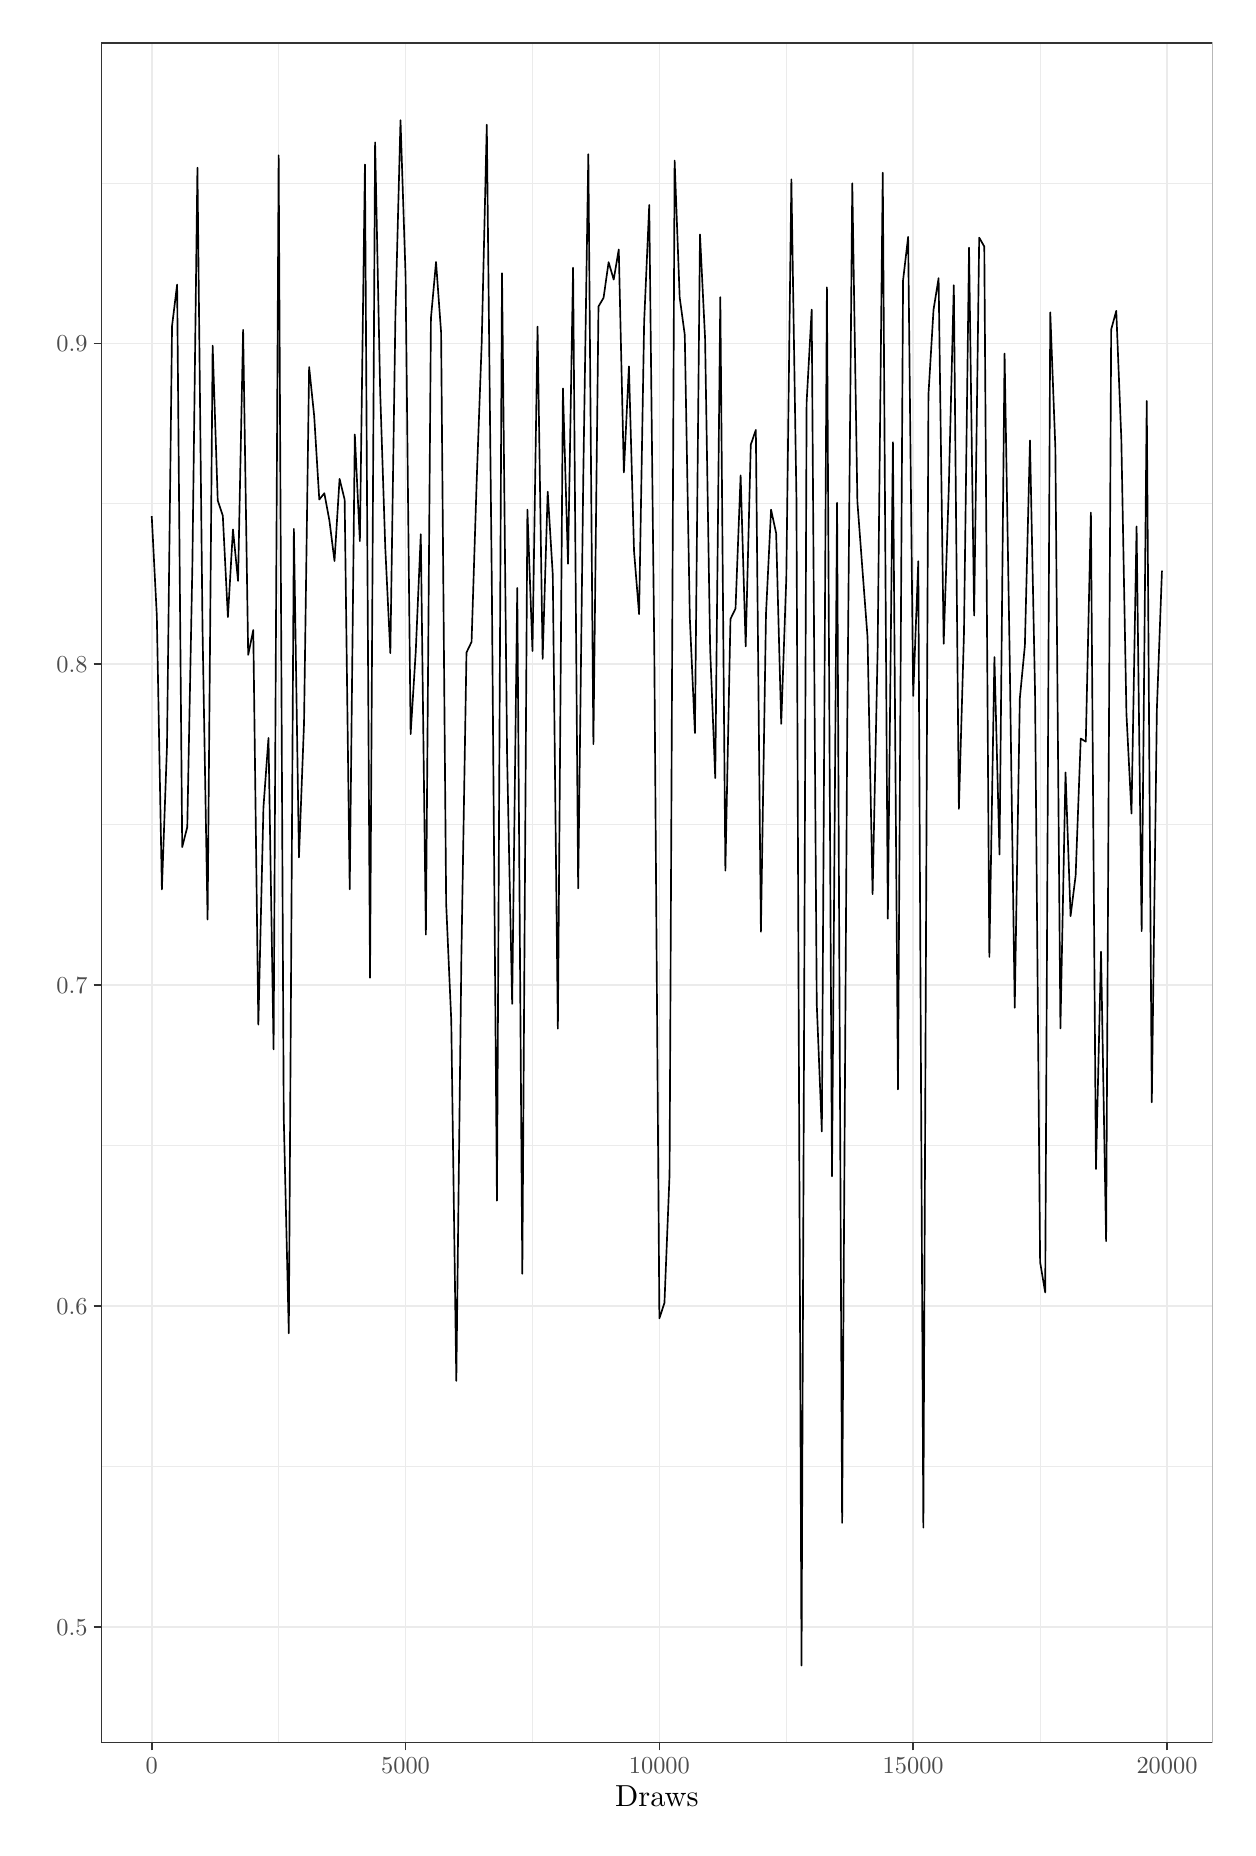
\begin{tikzpicture}[x=1pt,y=1pt]
\definecolor{fillColor}{RGB}{255,255,255}
\path[use as bounding box,fill=fillColor,fill opacity=0.00] (0,0) rectangle (433.62,650.43);
\begin{scope}
\path[clip] (  0.00,  0.00) rectangle (433.62,650.43);
\definecolor{drawColor}{RGB}{255,255,255}
\definecolor{fillColor}{RGB}{255,255,255}

\path[draw=drawColor,line width= 0.6pt,line join=round,line cap=round,fill=fillColor] (  0.00,  0.00) rectangle (433.62,650.43);
\end{scope}
\begin{scope}
\path[clip] ( 26.58, 30.69) rectangle (428.12,644.93);
\definecolor{fillColor}{RGB}{255,255,255}

\path[fill=fillColor] ( 26.58, 30.69) rectangle (428.12,644.93);
\definecolor{drawColor}{gray}{0.92}

\path[draw=drawColor,line width= 0.3pt,line join=round] ( 26.58,130.49) --
	(428.12,130.49);

\path[draw=drawColor,line width= 0.3pt,line join=round] ( 26.58,246.44) --
	(428.12,246.44);

\path[draw=drawColor,line width= 0.3pt,line join=round] ( 26.58,362.39) --
	(428.12,362.39);

\path[draw=drawColor,line width= 0.3pt,line join=round] ( 26.58,478.35) --
	(428.12,478.35);

\path[draw=drawColor,line width= 0.3pt,line join=round] ( 26.58,594.30) --
	(428.12,594.30);

\path[draw=drawColor,line width= 0.3pt,line join=round] ( 90.69, 30.69) --
	( 90.69,644.93);

\path[draw=drawColor,line width= 0.3pt,line join=round] (182.41, 30.69) --
	(182.41,644.93);

\path[draw=drawColor,line width= 0.3pt,line join=round] (274.13, 30.69) --
	(274.13,644.93);

\path[draw=drawColor,line width= 0.3pt,line join=round] (365.84, 30.69) --
	(365.84,644.93);

\path[draw=drawColor,line width= 0.6pt,line join=round] ( 26.58, 72.52) --
	(428.12, 72.52);

\path[draw=drawColor,line width= 0.6pt,line join=round] ( 26.58,188.47) --
	(428.12,188.47);

\path[draw=drawColor,line width= 0.6pt,line join=round] ( 26.58,304.42) --
	(428.12,304.42);

\path[draw=drawColor,line width= 0.6pt,line join=round] ( 26.58,420.37) --
	(428.12,420.37);

\path[draw=drawColor,line width= 0.6pt,line join=round] ( 26.58,536.32) --
	(428.12,536.32);

\path[draw=drawColor,line width= 0.6pt,line join=round] ( 44.83, 30.69) --
	( 44.83,644.93);

\path[draw=drawColor,line width= 0.6pt,line join=round] (136.55, 30.69) --
	(136.55,644.93);

\path[draw=drawColor,line width= 0.6pt,line join=round] (228.27, 30.69) --
	(228.27,644.93);

\path[draw=drawColor,line width= 0.6pt,line join=round] (319.98, 30.69) --
	(319.98,644.93);

\path[draw=drawColor,line width= 0.6pt,line join=round] (411.70, 30.69) --
	(411.70,644.93);
\definecolor{drawColor}{RGB}{0,0,0}

\path[draw=drawColor,line width= 0.6pt,line join=round] ( 44.83,473.93) --
	( 46.67,437.87) --
	( 48.50,339.03) --
	( 50.34,390.79) --
	( 52.17,542.64) --
	( 54.00,557.60) --
	( 55.84,354.33) --
	( 57.67,361.57) --
	( 59.51,455.94) --
	( 61.34,599.82) --
	( 63.18,433.32) --
	( 65.01,328.14) --
	( 66.84,535.51) --
	( 68.68,479.56) --
	( 70.51,474.12) --
	( 72.35,437.45) --
	( 74.18,469.11) --
	( 76.02,450.51) --
	( 77.85,541.22) --
	( 79.68,423.79) --
	( 81.52,432.77) --
	( 83.35,290.17) --
	( 85.19,368.61) --
	( 87.02,393.78) --
	( 88.86,281.24) --
	( 90.69,604.32) --
	( 92.53,256.83) --
	( 94.36,178.65) --
	( 96.19,469.30) --
	( 98.03,350.61) --
	( 99.86,399.11) --
	(101.70,527.81) --
	(103.53,510.13) --
	(105.37,479.93) --
	(107.20,482.18) --
	(109.03,472.35) --
	(110.87,457.70) --
	(112.70,487.38) --
	(114.54,479.87) --
	(116.37,339.10) --
	(118.21,503.42) --
	(120.04,464.89) --
	(121.87,600.97) --
	(123.71,307.11) --
	(125.54,608.97) --
	(127.38,518.80) --
	(129.21,462.70) --
	(131.05,424.41) --
	(132.88,546.33) --
	(134.72,617.01) --
	(136.55,560.97) --
	(138.38,395.16) --
	(140.22,424.78) --
	(142.05,467.40) --
	(143.89,322.71) --
	(145.72,545.49) --
	(147.56,565.75) --
	(149.39,540.29) --
	(151.22,333.87) --
	(153.06,291.68) --
	(154.89,161.44) --
	(156.73,315.53) --
	(158.56,424.64) --
	(160.40,428.48) --
	(162.23,486.14) --
	(164.06,536.58) --
	(165.90,615.35) --
	(167.73,447.94) --
	(169.57,226.55) --
	(171.40,561.68) --
	(173.24,387.19) --
	(175.07,297.67) --
	(176.91,448.00) --
	(178.74,200.13) --
	(180.57,476.26) --
	(182.41,425.18) --
	(184.24,542.40) --
	(186.08,422.36) --
	(187.91,482.75) --
	(189.75,452.64) --
	(191.58,288.68) --
	(193.41,520.05) --
	(195.25,456.67) --
	(197.08,563.68) --
	(198.92,339.42) --
	(200.75,486.87) --
	(202.59,604.71) --
	(204.42,391.49) --
	(206.26,549.69) --
	(208.09,552.80) --
	(209.92,565.68) --
	(211.76,559.40) --
	(213.59,570.29) --
	(215.43,489.71) --
	(217.26,528.02) --
	(219.10,461.36) --
	(220.93,438.53) --
	(222.76,544.10) --
	(224.60,586.32) --
	(226.43,424.91) --
	(228.27,184.04) --
	(230.10,189.64) --
	(231.94,235.93) --
	(233.77,602.43) --
	(235.60,552.96) --
	(237.44,539.42) --
	(239.27,437.00) --
	(241.11,395.53) --
	(242.94,575.68) --
	(244.78,538.06) --
	(246.61,425.99) --
	(248.45,379.24) --
	(250.28,553.05) --
	(252.11,345.81) --
	(253.95,436.75) --
	(255.78,440.53) --
	(257.62,488.66) --
	(259.45,426.86) --
	(261.29,499.72) --
	(263.12,505.08) --
	(264.95,323.73) --
	(266.79,438.58) --
	(268.62,476.26) --
	(270.46,467.74) --
	(272.29,398.84) --
	(274.13,451.66) --
	(275.96,595.60) --
	(277.79,480.17) --
	(279.63, 58.61) --
	(281.46,514.85) --
	(283.30,548.55) --
	(285.13,297.64) --
	(286.97,251.55) --
	(288.80,556.60) --
	(290.64,235.41) --
	(292.47,478.74) --
	(294.30,110.16) --
	(296.14,396.78) --
	(297.97,594.18) --
	(299.81,479.15) --
	(301.64,454.61) --
	(303.48,430.18) --
	(305.31,337.32) --
	(307.14,426.19) --
	(308.98,598.00) --
	(310.81,328.46) --
	(312.65,500.62) --
	(314.48,266.77) --
	(316.32,559.14) --
	(318.15,574.81) --
	(319.98,408.94) --
	(321.82,457.61) --
	(323.65,108.44) --
	(325.49,517.81) --
	(327.32,548.46) --
	(329.16,559.91) --
	(330.99,427.78) --
	(332.83,483.55) --
	(334.66,557.35) --
	(336.49,368.16) --
	(338.33,431.68) --
	(340.16,570.94) --
	(342.00,438.00) --
	(343.83,574.55) --
	(345.67,571.34) --
	(347.50,314.63) --
	(349.33,422.99) --
	(351.17,351.65) --
	(353.00,532.68) --
	(354.84,423.53) --
	(356.67,296.28) --
	(358.51,408.04) --
	(360.34,427.19) --
	(362.18,501.27) --
	(364.01,410.35) --
	(365.84,204.35) --
	(367.68,193.41) --
	(369.51,547.56) --
	(371.35,498.56) --
	(373.18,288.80) --
	(375.02,381.33) --
	(376.85,329.39) --
	(378.68,344.05) --
	(380.52,393.55) --
	(382.35,392.43) --
	(384.19,475.23) --
	(386.02,238.01) --
	(387.86,316.50) --
	(389.69,211.90) --
	(391.52,541.36) --
	(393.36,548.10) --
	(395.19,501.70) --
	(397.03,402.57) --
	(398.86,366.48) --
	(400.70,470.20) --
	(402.53,323.97) --
	(404.37,515.50) --
	(406.20,262.13) --
	(408.03,404.12) --
	(409.87,454.21);
\definecolor{drawColor}{gray}{0.20}

\path[draw=drawColor,line width= 0.6pt,line join=round,line cap=round] ( 26.58, 30.69) rectangle (428.12,644.93);
\end{scope}
\begin{scope}
\path[clip] (  0.00,  0.00) rectangle (433.62,650.43);
\definecolor{drawColor}{gray}{0.30}

\node[text=drawColor,anchor=base east,inner sep=0pt, outer sep=0pt, scale=  0.88] at ( 21.63, 69.49) {0.5};

\node[text=drawColor,anchor=base east,inner sep=0pt, outer sep=0pt, scale=  0.88] at ( 21.63,185.44) {0.6};

\node[text=drawColor,anchor=base east,inner sep=0pt, outer sep=0pt, scale=  0.88] at ( 21.63,301.39) {0.7};

\node[text=drawColor,anchor=base east,inner sep=0pt, outer sep=0pt, scale=  0.88] at ( 21.63,417.34) {0.8};

\node[text=drawColor,anchor=base east,inner sep=0pt, outer sep=0pt, scale=  0.88] at ( 21.63,533.29) {0.9};
\end{scope}
\begin{scope}
\path[clip] (  0.00,  0.00) rectangle (433.62,650.43);
\definecolor{drawColor}{gray}{0.20}

\path[draw=drawColor,line width= 0.6pt,line join=round] ( 23.83, 72.52) --
	( 26.58, 72.52);

\path[draw=drawColor,line width= 0.6pt,line join=round] ( 23.83,188.47) --
	( 26.58,188.47);

\path[draw=drawColor,line width= 0.6pt,line join=round] ( 23.83,304.42) --
	( 26.58,304.42);

\path[draw=drawColor,line width= 0.6pt,line join=round] ( 23.83,420.37) --
	( 26.58,420.37);

\path[draw=drawColor,line width= 0.6pt,line join=round] ( 23.83,536.32) --
	( 26.58,536.32);
\end{scope}
\begin{scope}
\path[clip] (  0.00,  0.00) rectangle (433.62,650.43);
\definecolor{drawColor}{gray}{0.20}

\path[draw=drawColor,line width= 0.6pt,line join=round] ( 44.83, 27.94) --
	( 44.83, 30.69);

\path[draw=drawColor,line width= 0.6pt,line join=round] (136.55, 27.94) --
	(136.55, 30.69);

\path[draw=drawColor,line width= 0.6pt,line join=round] (228.27, 27.94) --
	(228.27, 30.69);

\path[draw=drawColor,line width= 0.6pt,line join=round] (319.98, 27.94) --
	(319.98, 30.69);

\path[draw=drawColor,line width= 0.6pt,line join=round] (411.70, 27.94) --
	(411.70, 30.69);
\end{scope}
\begin{scope}
\path[clip] (  0.00,  0.00) rectangle (433.62,650.43);
\definecolor{drawColor}{gray}{0.30}

\node[text=drawColor,anchor=base,inner sep=0pt, outer sep=0pt, scale=  0.88] at ( 44.83, 19.68) {0};

\node[text=drawColor,anchor=base,inner sep=0pt, outer sep=0pt, scale=  0.88] at (136.55, 19.68) {5000};

\node[text=drawColor,anchor=base,inner sep=0pt, outer sep=0pt, scale=  0.88] at (228.27, 19.68) {10000};

\node[text=drawColor,anchor=base,inner sep=0pt, outer sep=0pt, scale=  0.88] at (319.98, 19.68) {15000};

\node[text=drawColor,anchor=base,inner sep=0pt, outer sep=0pt, scale=  0.88] at (411.70, 19.68) {20000};
\end{scope}
\begin{scope}
\path[clip] (  0.00,  0.00) rectangle (433.62,650.43);
\definecolor{drawColor}{RGB}{0,0,0}

\node[text=drawColor,anchor=base,inner sep=0pt, outer sep=0pt, scale=  1.10] at (227.35,  7.64) {Draws};
\end{scope}
\end{tikzpicture}
